\documentclass[letterpaper,14pt,titlepage,fleqn]{article}

\setlength{\mathindent}{1cm}

\usepackage{graphicx}                                        

\usepackage{amssymb}                                         
\usepackage{amsmath}                                         
\usepackage{amsthm}                                          

\usepackage{alltt}                                           
\usepackage{float}
\usepackage{color}

\usepackage{url}

\usepackage{balance}
\usepackage[TABBOTCAP, tight]{subfigure}
\usepackage{enumitem}

\usepackage{pstricks, pst-node}

\usepackage{cite}
\usepackage{indentfirst}
\usepackage{listings}

% the following sets the geometry of the page
\usepackage{geometry}
\geometry{textheight=9in, textwidth=6.5in}

% random comment

\newcommand{\cred}[1]{{\color{red}#1}}
\newcommand{\cblue}[1]{{\color{blue}#1}}

\usepackage{hyperref}

\usepackage{textcomp}
\usepackage{listings}

\def\name{Haoxiang Wang; Student ID: 932359049}

%% The following metadata will show up in the PDF properties
\hypersetup{
  colorlinks = true,
  urlcolor = black,
  pdfauthor = {\name},
  pdfkeywords = {CS557 Final Project},
  pdftitle = {Final Project: Simulation of Water Morphological Changes},
  pdfsubject = {Final Project: Simulation of Water Morphological Changes},
  pdfpagemode = UseNone
}

\parindent = 0.0 in
\parskip = 0.2 in

\author{\name}
\title{Final Project: Simulation of Water Morphological Changes}

\begin{document}
\maketitle
\begin{center}
	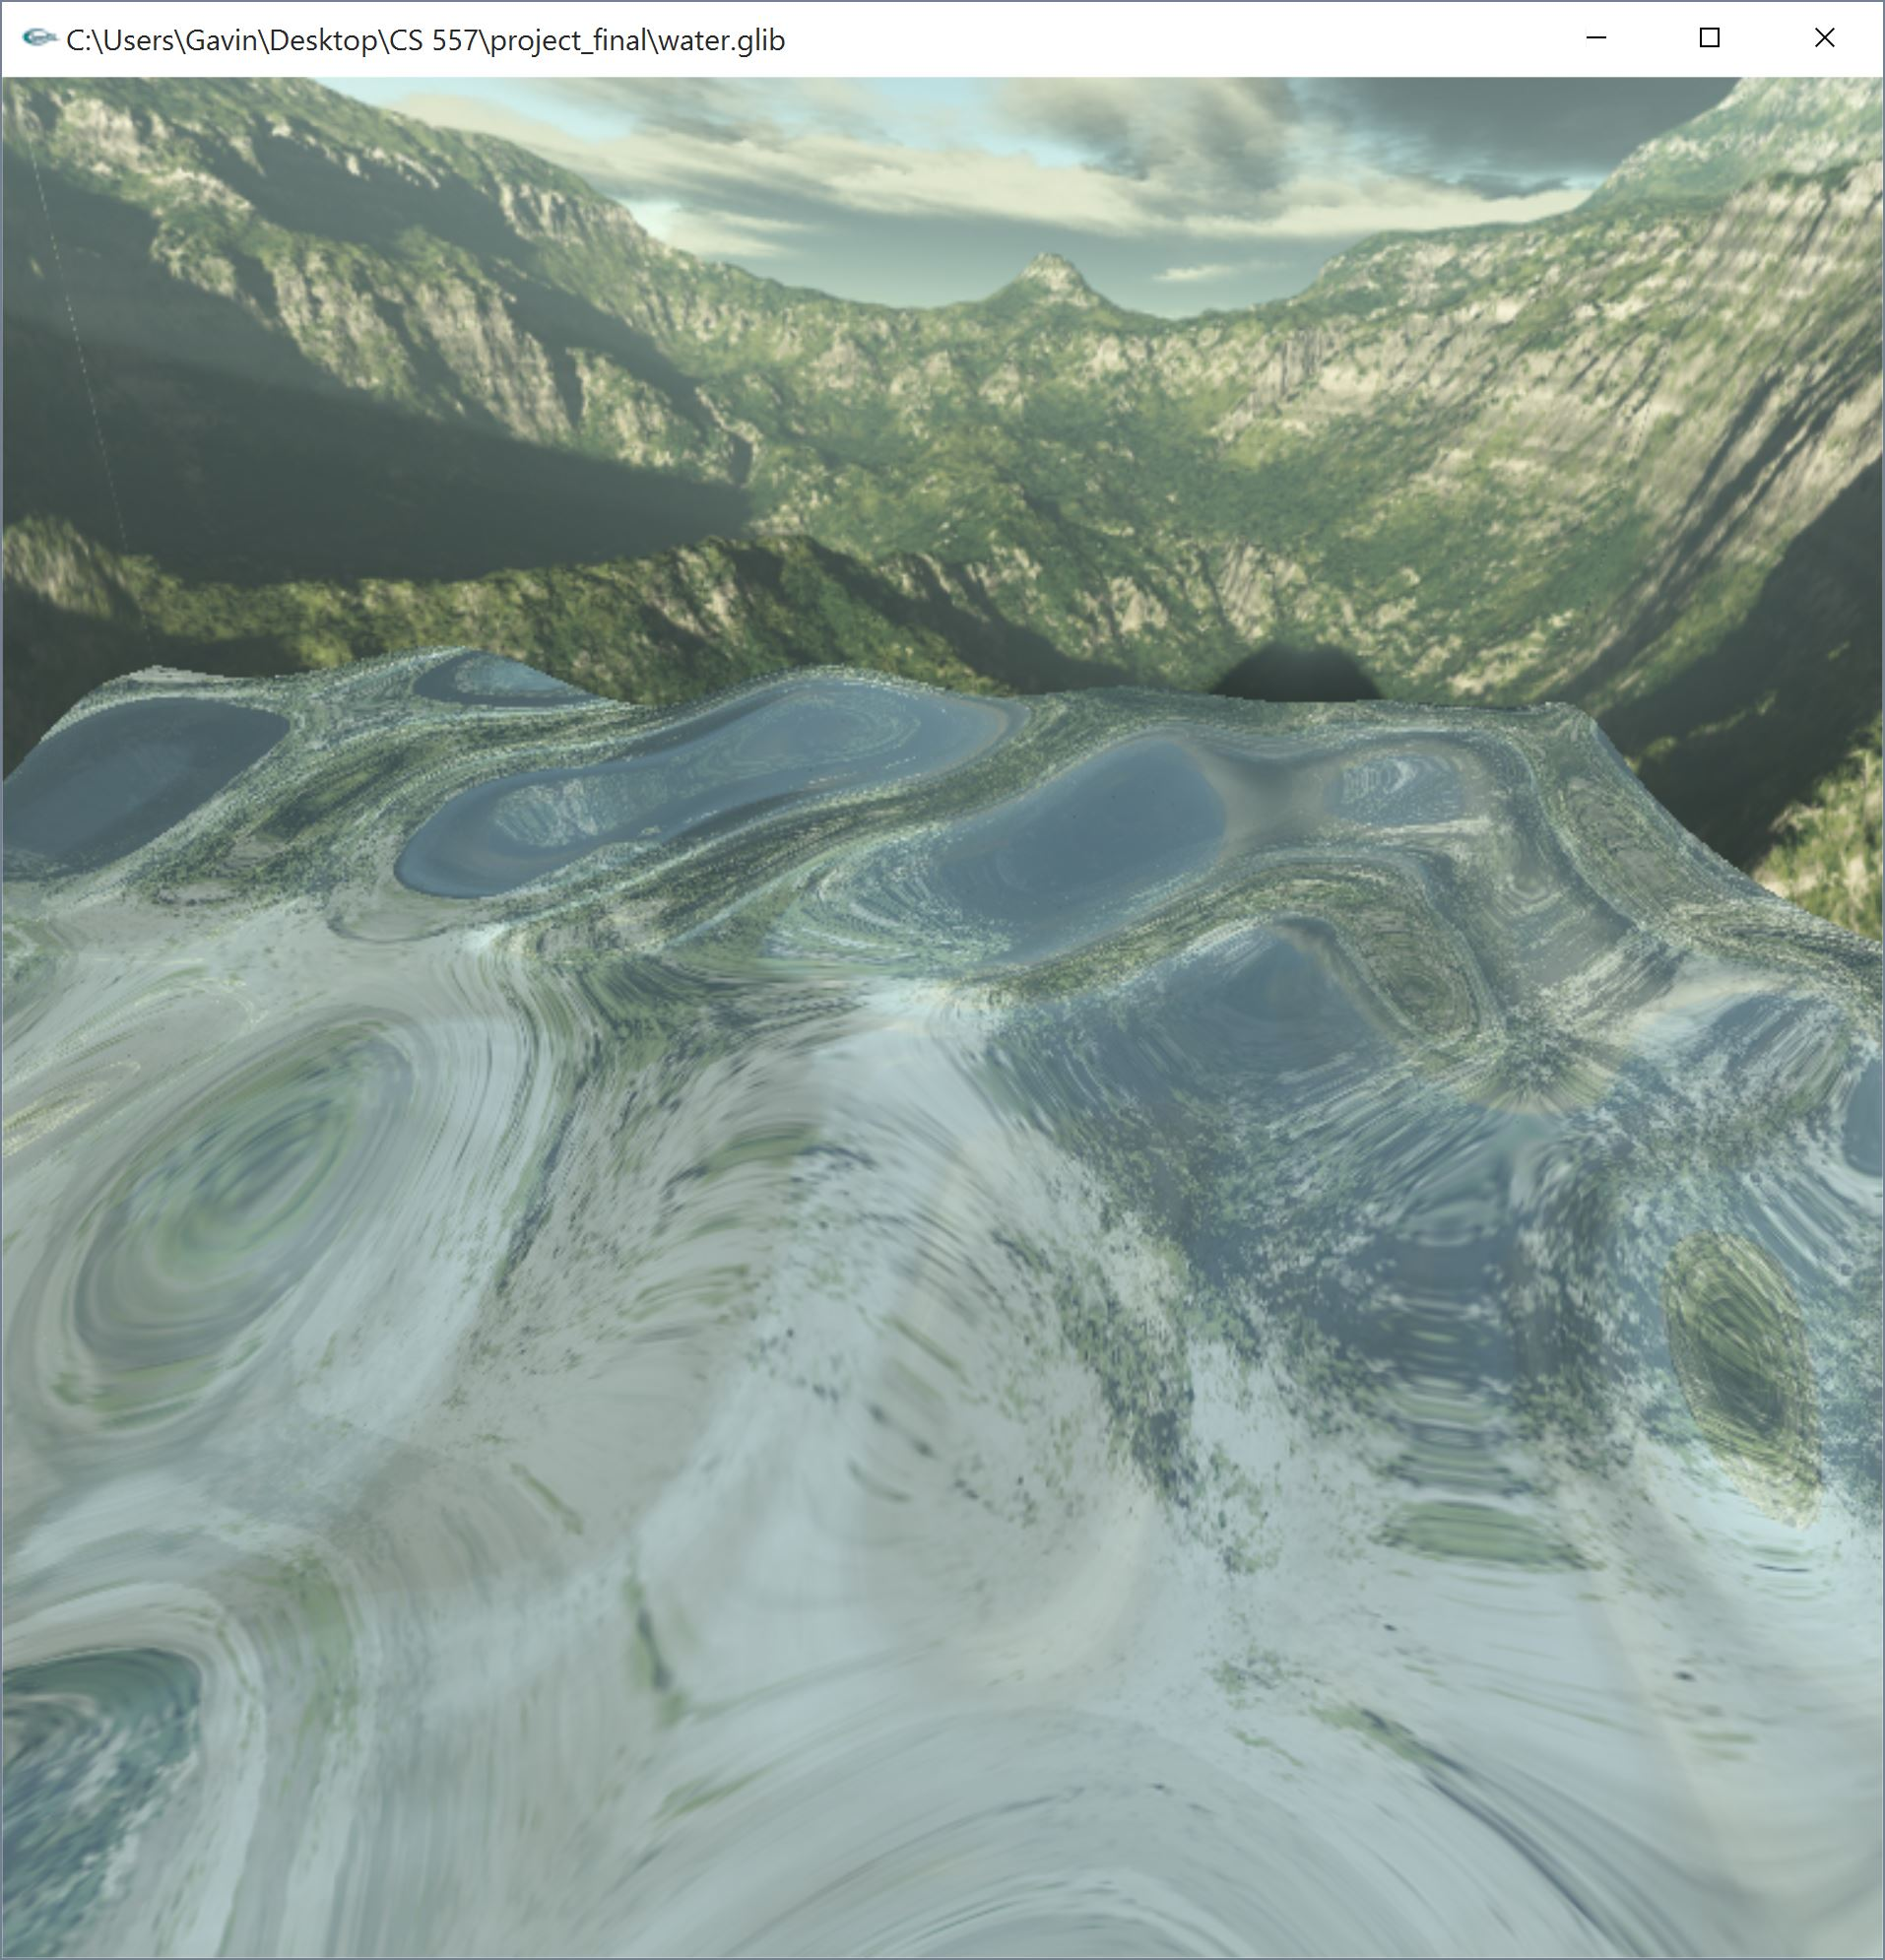
\includegraphics[width=4.5in]{final1.jpg}
\end{center}
This project is the final project I have done in this class, and I have done massive work on this one trying to reach the finest effects. However, comparing what I have implemented to want I wrote in the proposal, I cut off some of the bonus features due to the time issue but the main implement remains the same. The general idea of this project is to implement a simulation of water morphological changes. This involves the fluid simulation on water, the ice simulation and the fake cloud simulation. All of these three effects relate to a temperature variable controlled by a slider. The results images and the explanation of how code works will be described in the after section. 

\section{Source Listing}
In this project, eleven files are necessary. They are files handle the cube-mapping, files handle the water surface displacement, the effects and morphological changes rendering, and the textures. The specific filenames and usages are listed below.

water.glib --- Handle the user interface and all of the programs\\
water.vert --- Handle the vertex shader\\
water.frag --- Handle the fragment shader\\
texture.vert --- Handle cube-mapping\\
texture.frag --- Handle cube-mapping\\
cubeFront.bmp, cubeBack.bmp, cubeLeft.bmp, cubeRight.bmp,..\\
  ..cubeTop.bmp, cubeGround.bmp --- Cube-mapping textures

\section{Result Images and Explanation}
This project was not constructed from the ground. Several other projects and resources are used during the implementing. The techniques getting involved are Water simulation in GLSL \cite{waterSimu}, bump mapping, noise, mixing, cube mapping, reflection, and refraction. Only vertex shader and fragment shader are used. The displace ment of the water surface is done in the vertex shader based on a 200-by-200 quad. The ``fake'' reflection and refraction are implemented instead of applying the real ray tracing. 

Several uniform values are set in the program and controlled by sliders. They are uTimeScale for scaling the speed of the water waves, uEta and uMix for reflection and refraction implementing, uWaterHeight for changing the water surface's height, uNumWaves for changing the number of water waves added together, and uTemp for changing the temperature. The following image shows the original scene once the .glib file is executed. The water surface is drawn ar the $y=0$ position, so the original viewpoint is under the surface, but the refraction of the surface is obviouse due to the distortion of the texture.
\begin{center}
	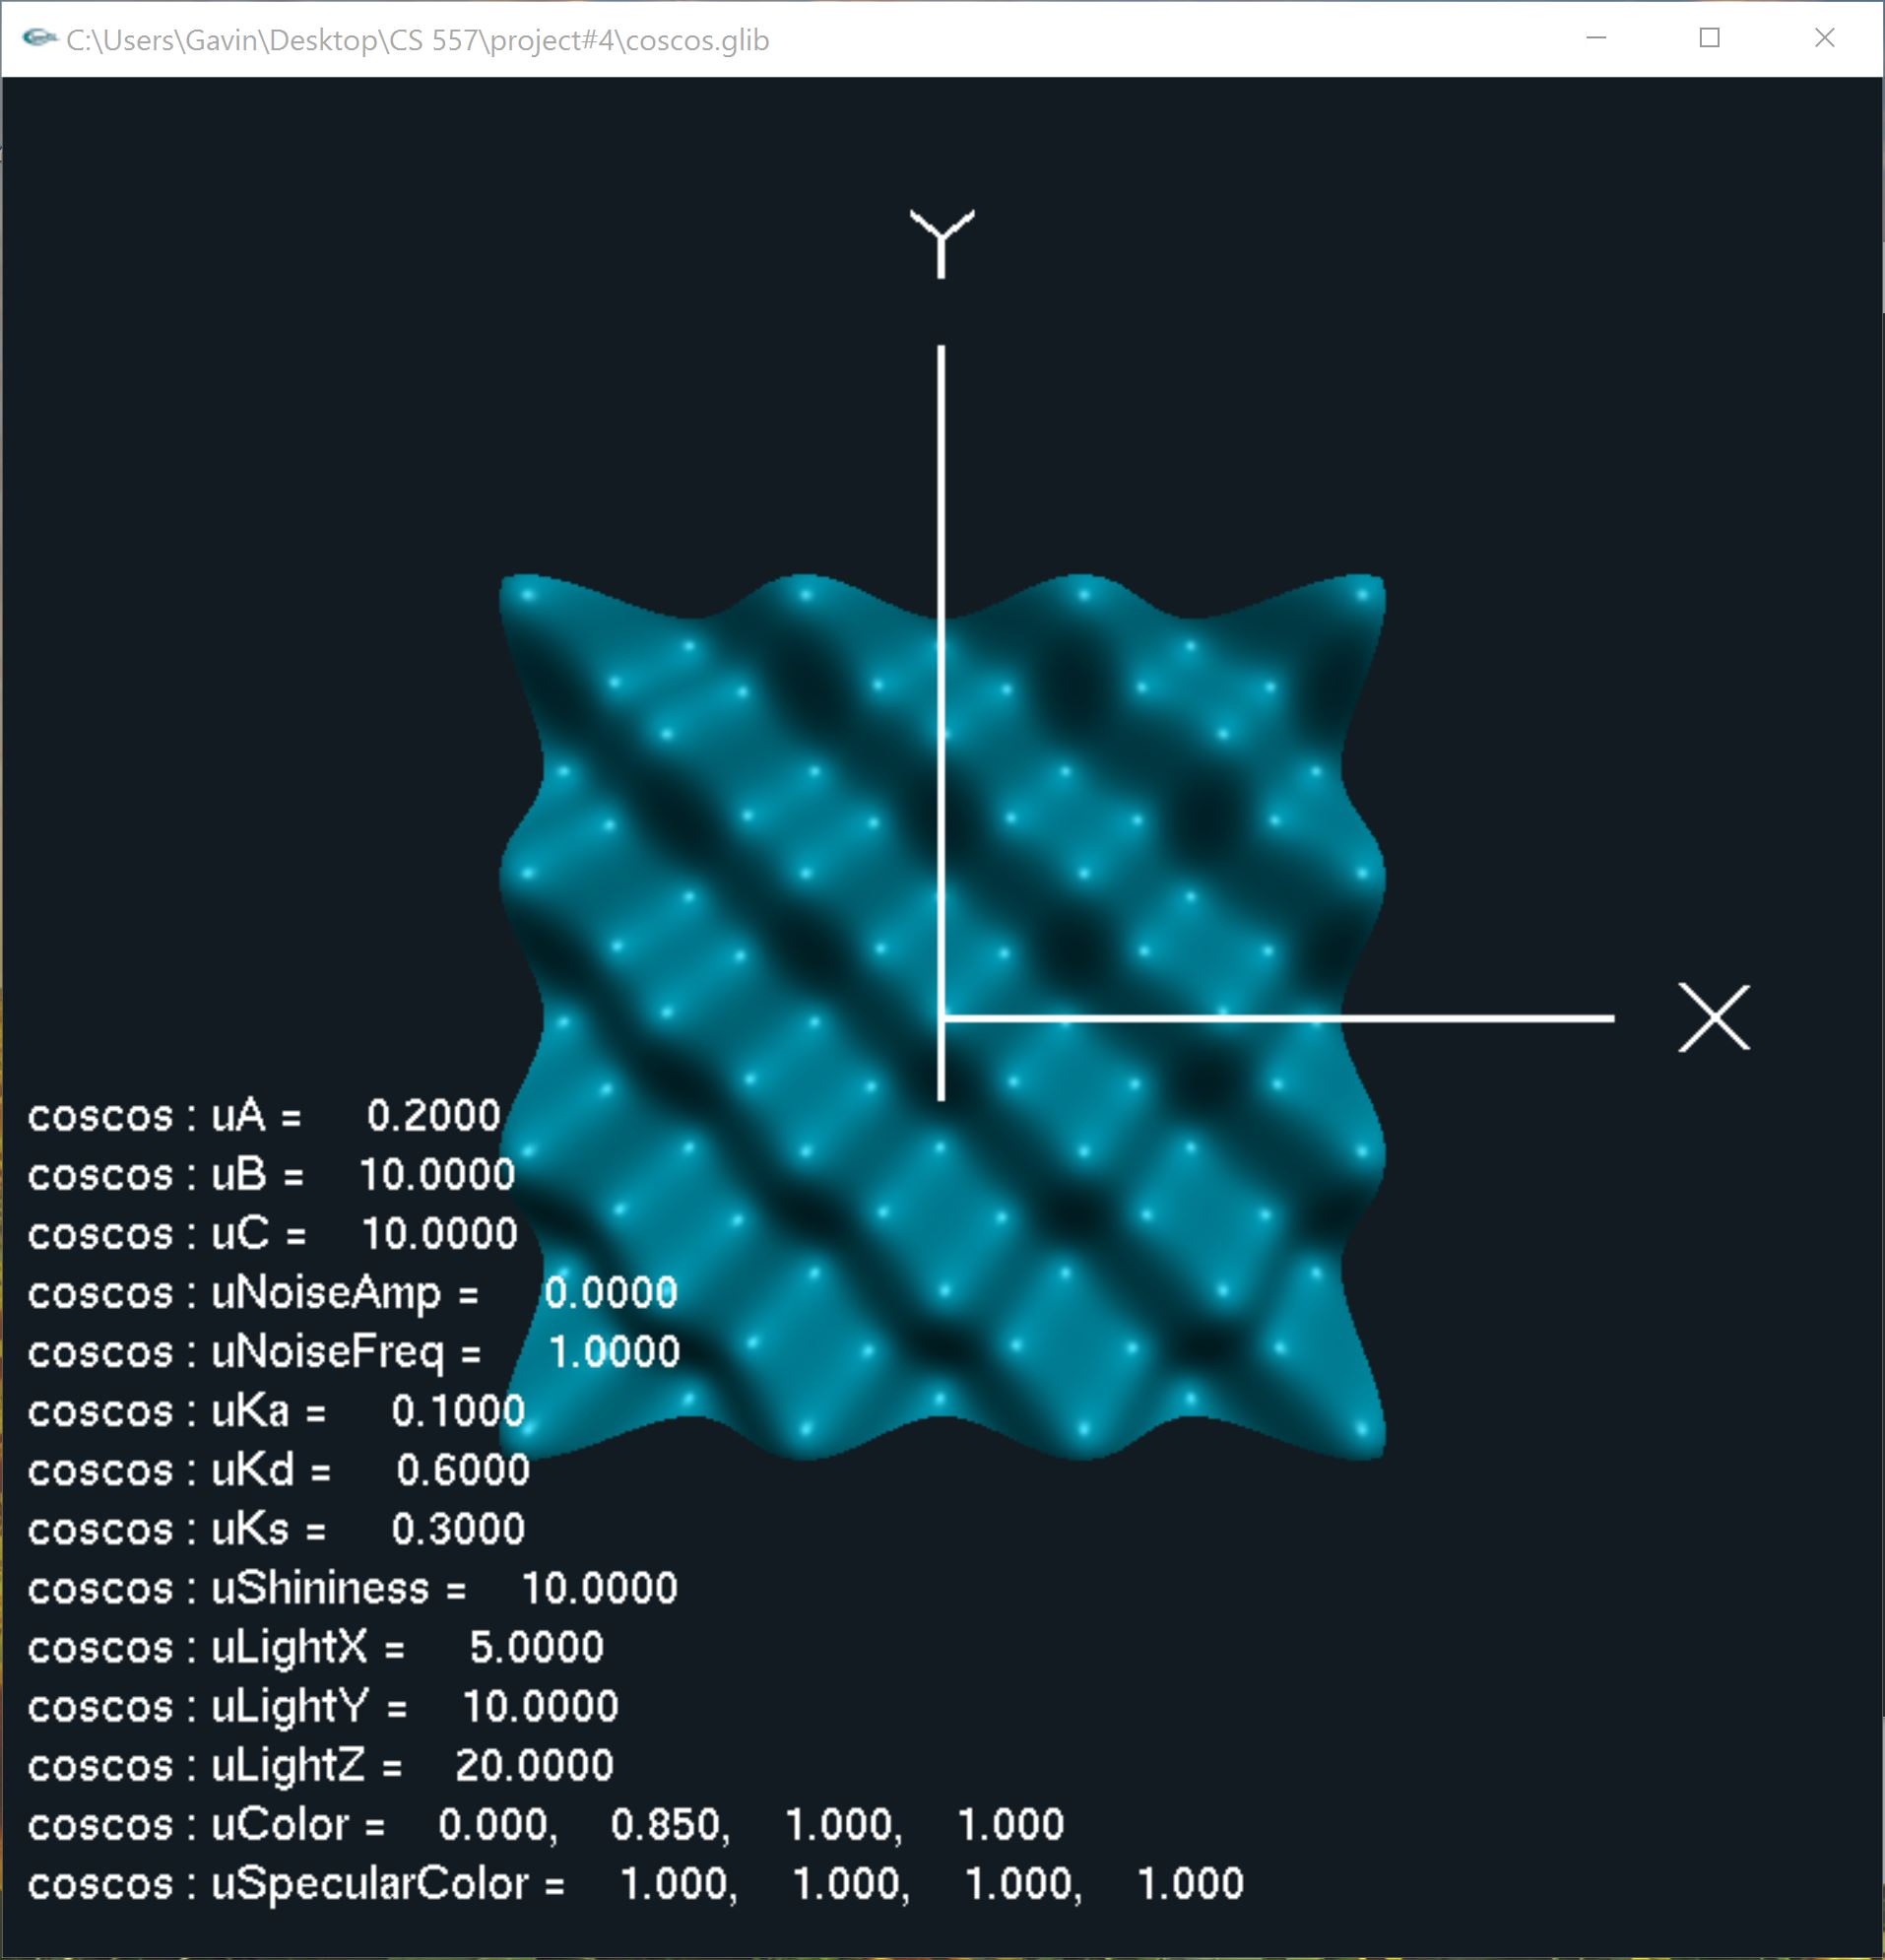
\includegraphics[width=4in]{origin.jpg}
\end{center}
As it shown at the very beginning of the report, the water surface has a complicated wave attached on. That wave is created by 4 individual sin waves with different directions, wave lengths, amplitudes, and speeds. The idea of adding several sin waves together to create the water wave comes from the idea in \cite{waterSimu}, and the implementing method is also mentioned in equation form in \cite{RealTime}. To calculating the new normal for the displaced surface, I calculated the derivative of the wave equation based on both x and z, then used them as the x and z component in the normal vector. The equation for water waves is $H(x,z,t) = \Sigma (A_i\times sin(D_i\cdot(x,z)\times {\omega}_i+t\times {\varphi}_i))$ and the normal equation is $N(x,z) = (-\dfrac{\partial}{\partial x}(H(x,z,t)),1,-\dfrac{\partial}{\partial z}(H(x,z,t)))$ \cite{RealTime}. By summing the waves together, the complex water wave could be created. The following 4 images shows the water wave contains 0 to 3 waves, and the image at the very beginning contains 4 waves.
\begin{center}
	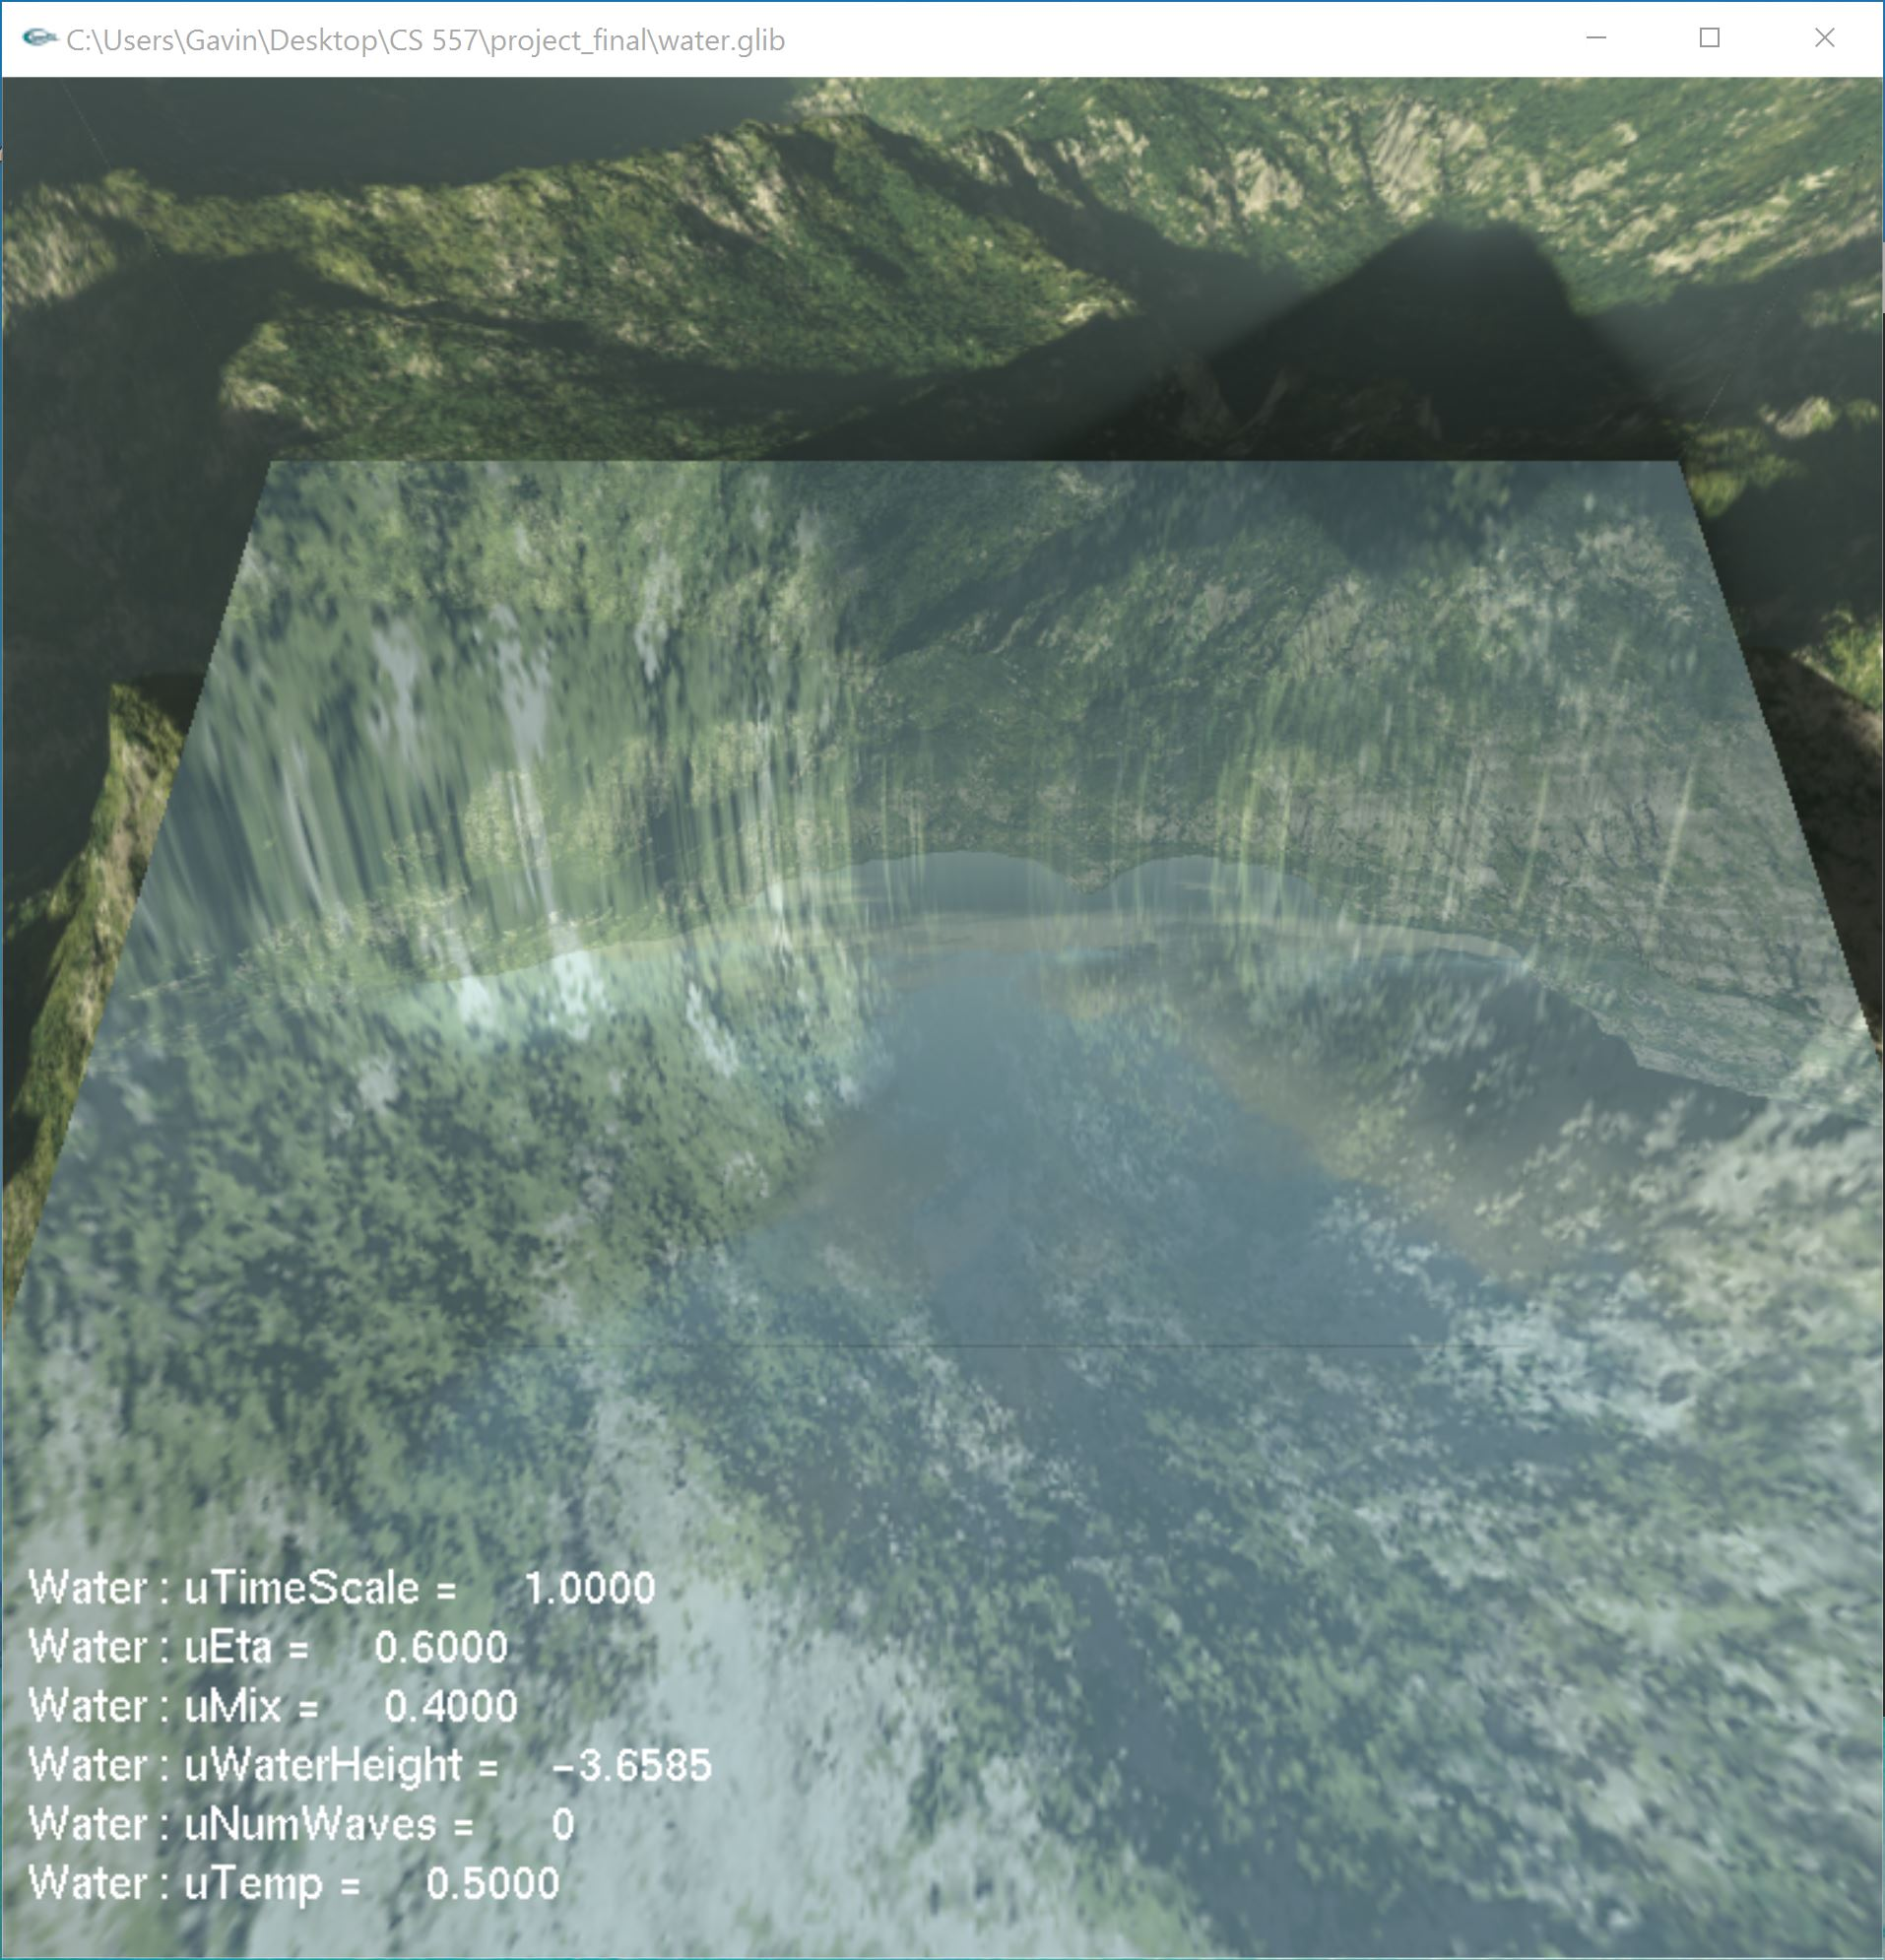
\includegraphics[width=3.2in]{wave0.jpg}
	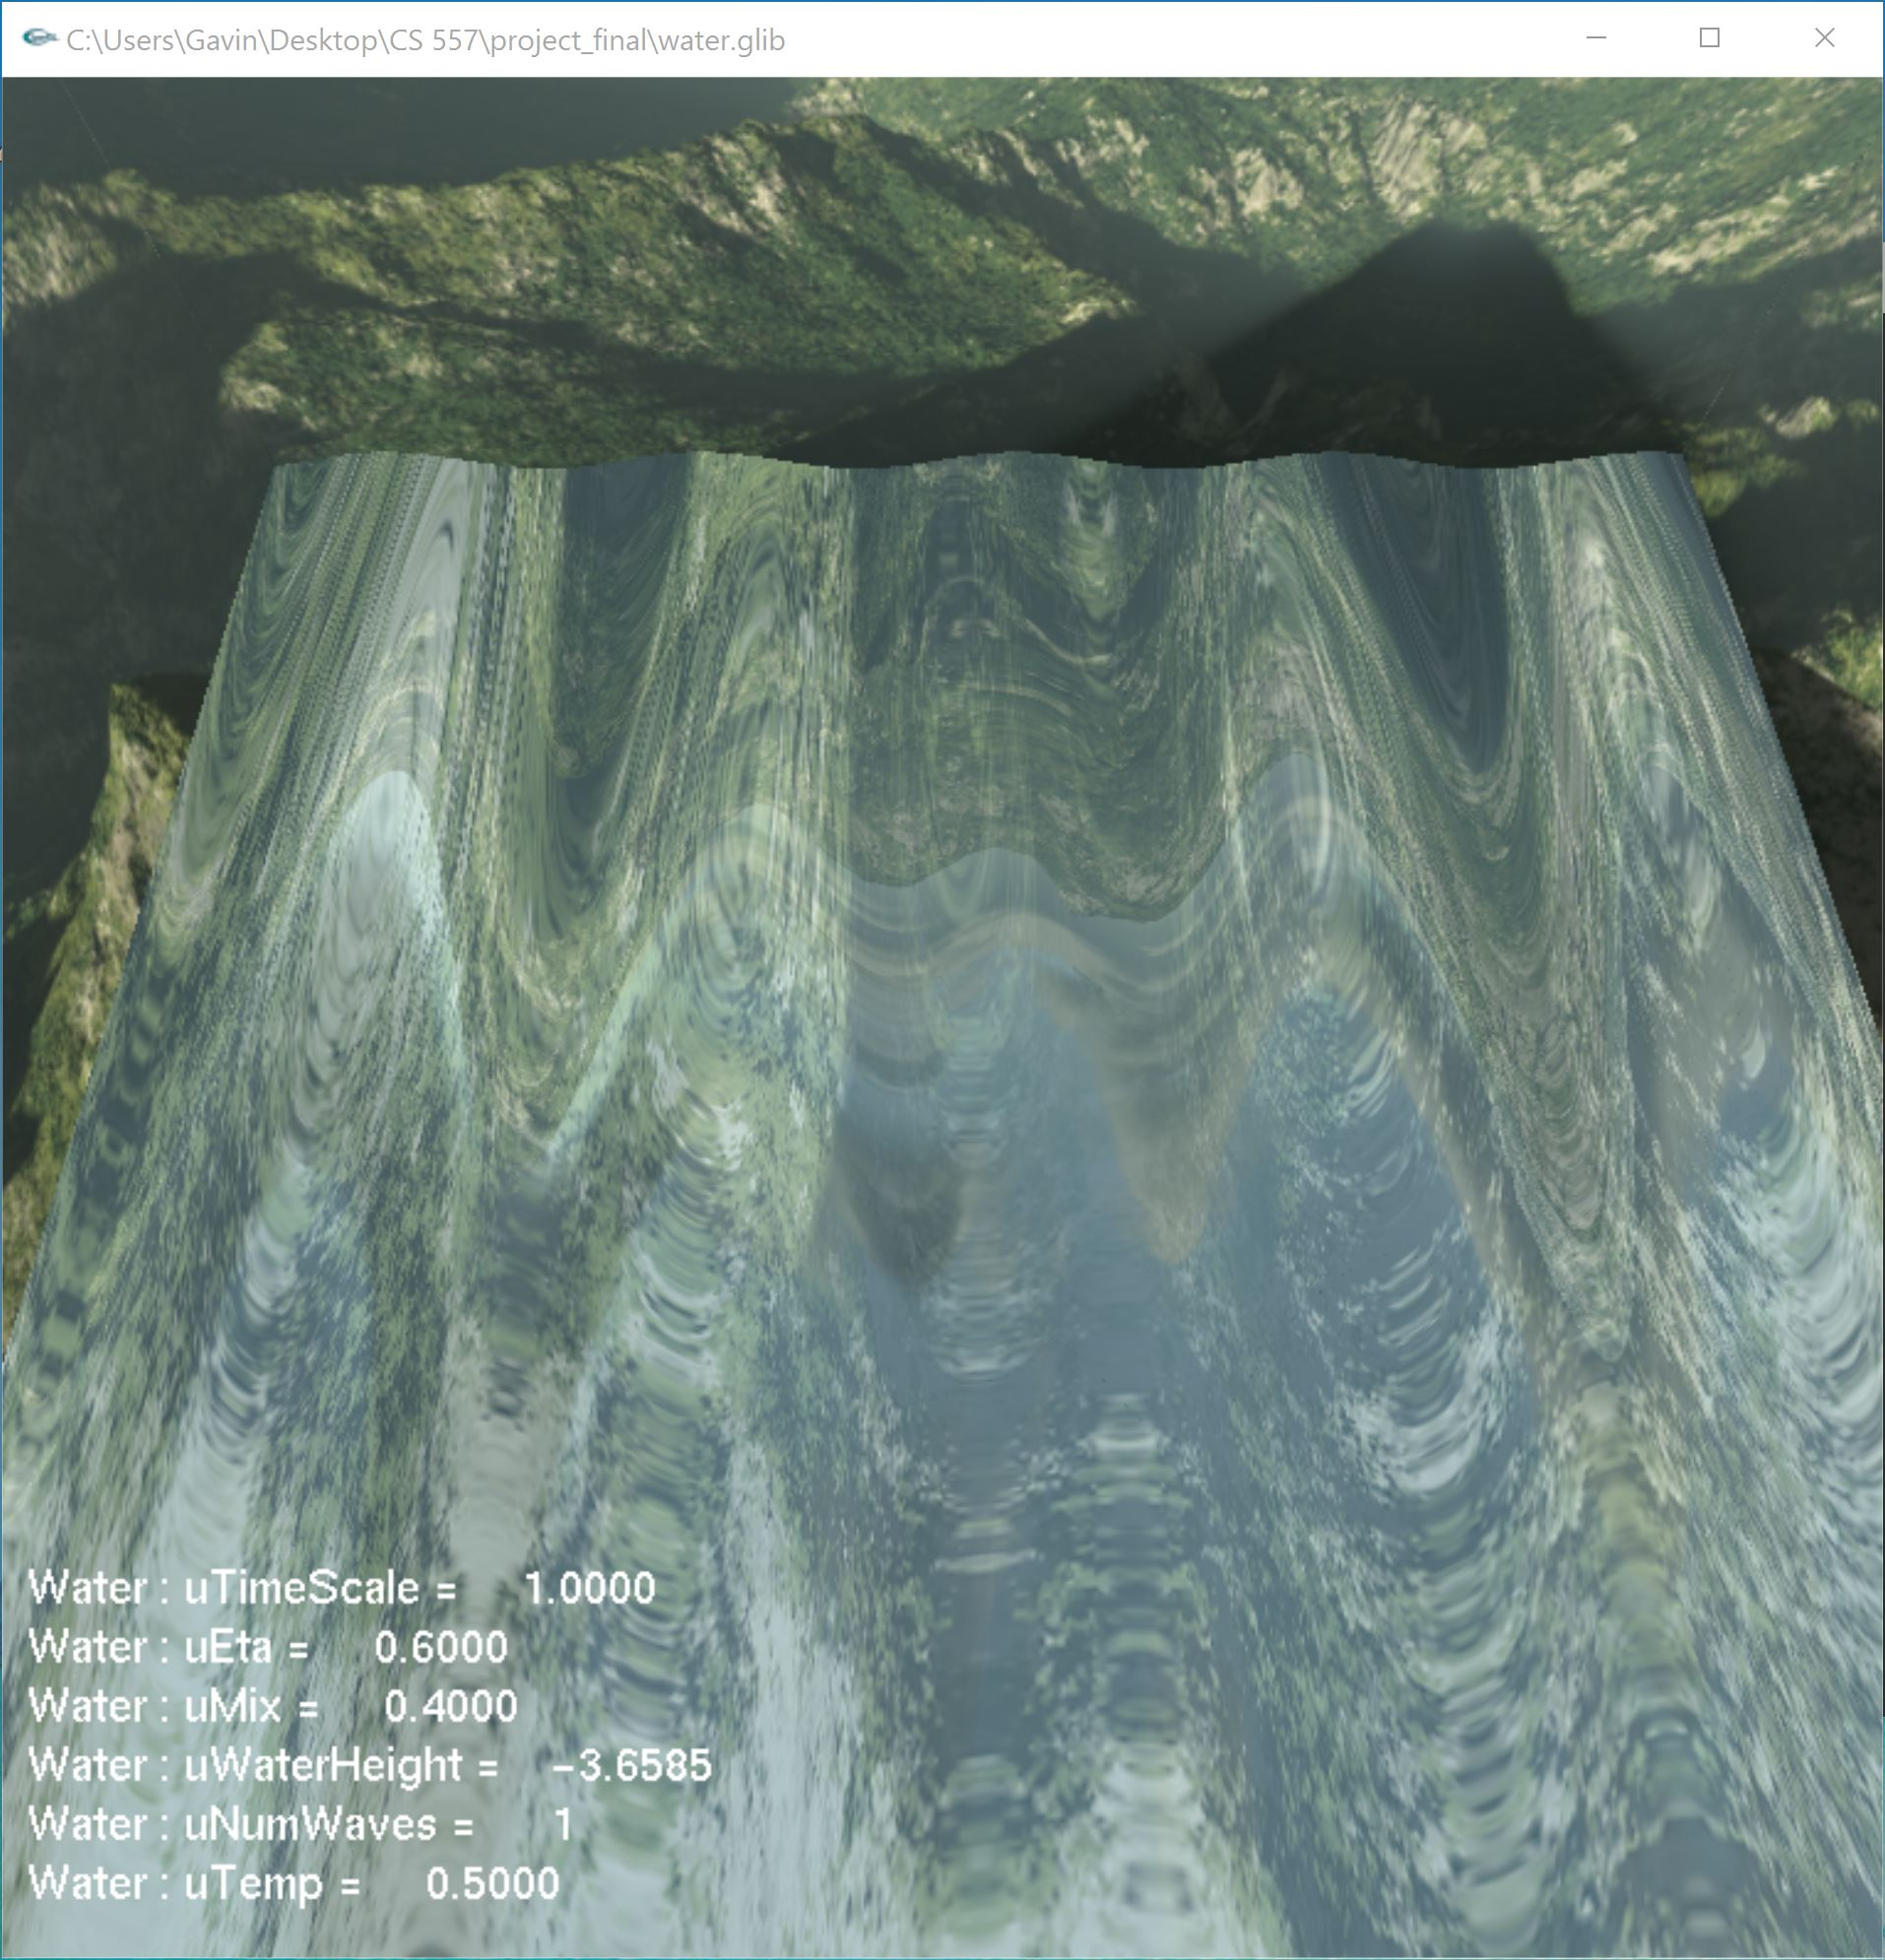
\includegraphics[width=3.2in]{wave1.jpg}
	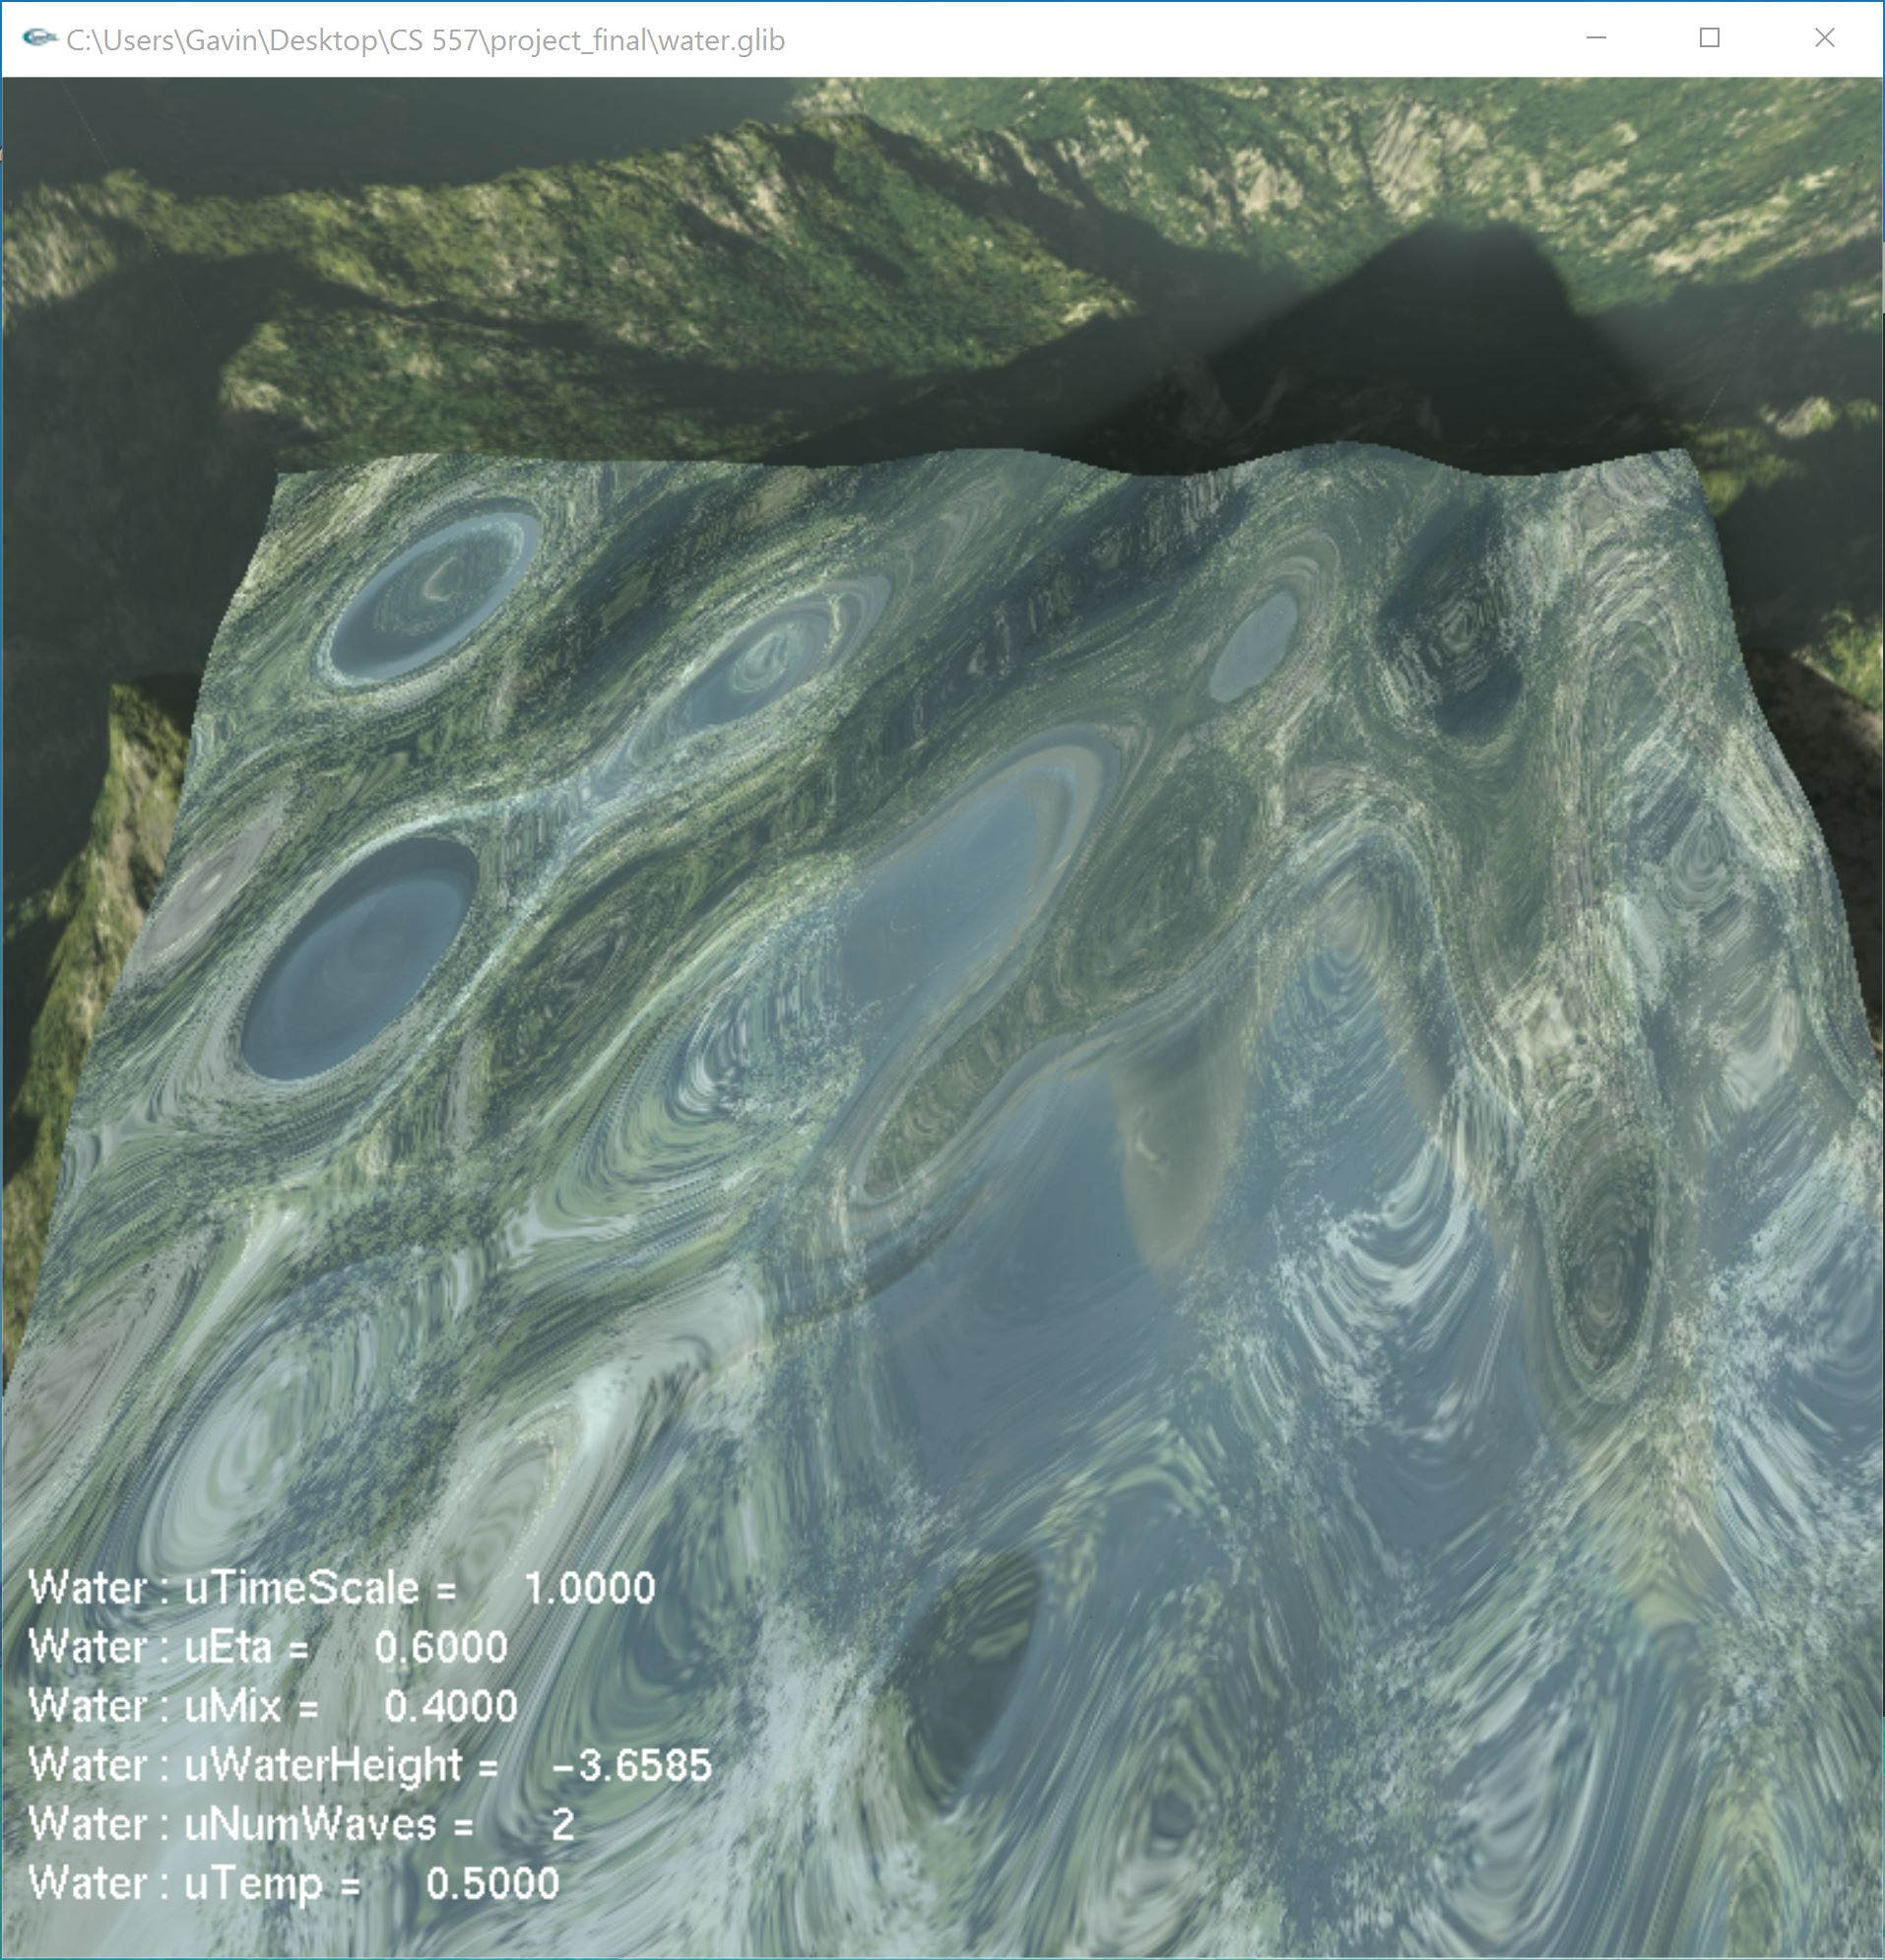
\includegraphics[width=3.2in]{wave2.jpg}
	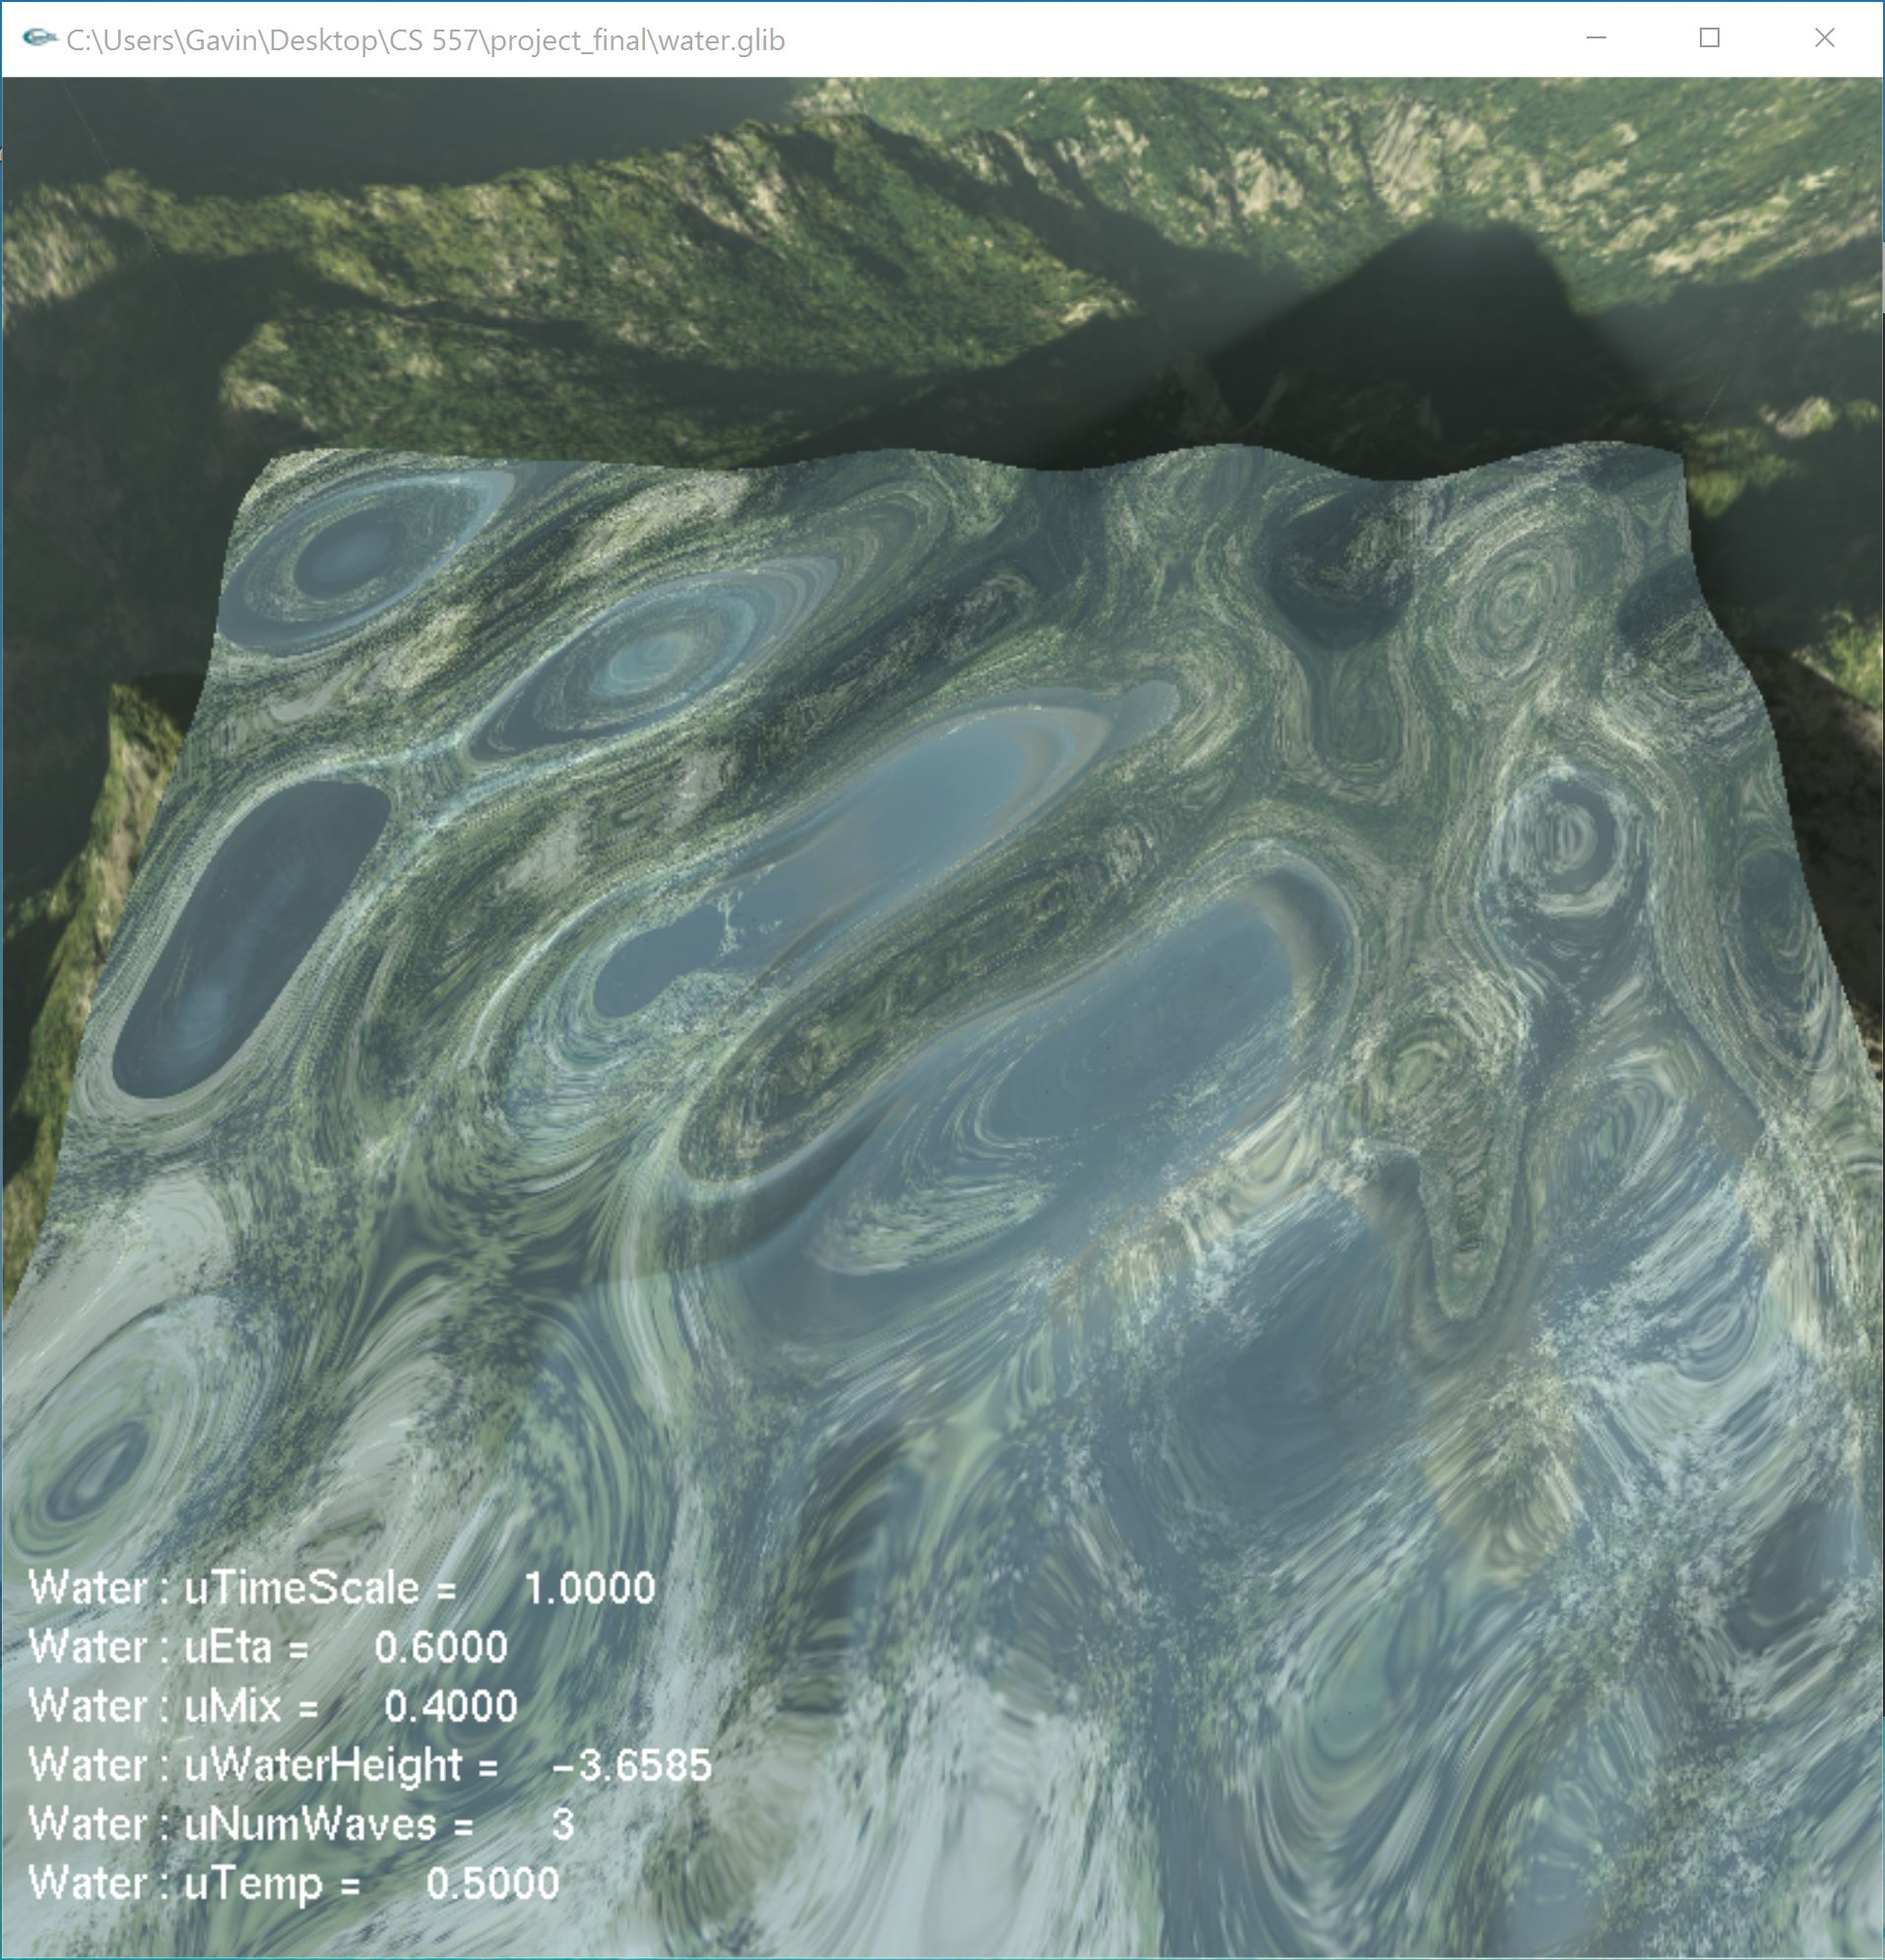
\includegraphics[width=3.2in]{wave3.jpg}
\end{center}
The reflection and the refraction are implemented based on the cube mapping. Since the real ray tracing is not implemented, the effect on the water surface is not real. However, it's good enough to deliver the water surface's feeling. Teh uMix value controlled by a slider determines how much reflection and how much refraction is getting blended. By setting uMix to 0 the water surface will only contain refraction, and by setting it to one, it will only contain reflection. The original value is set to 0.4 and can deliver a good effect. It should be mentioned that the water surface also gets some other color blened into it in order to make it looks more realistic. By testing with the color picker provided by glMan, the color $WATERCOLOR = vec3( .6, .85, 1. )$ becomes a good choice. The following 2 images show the effects that the surface only contains refraction (left) and reflection (right). 
\begin{center}
	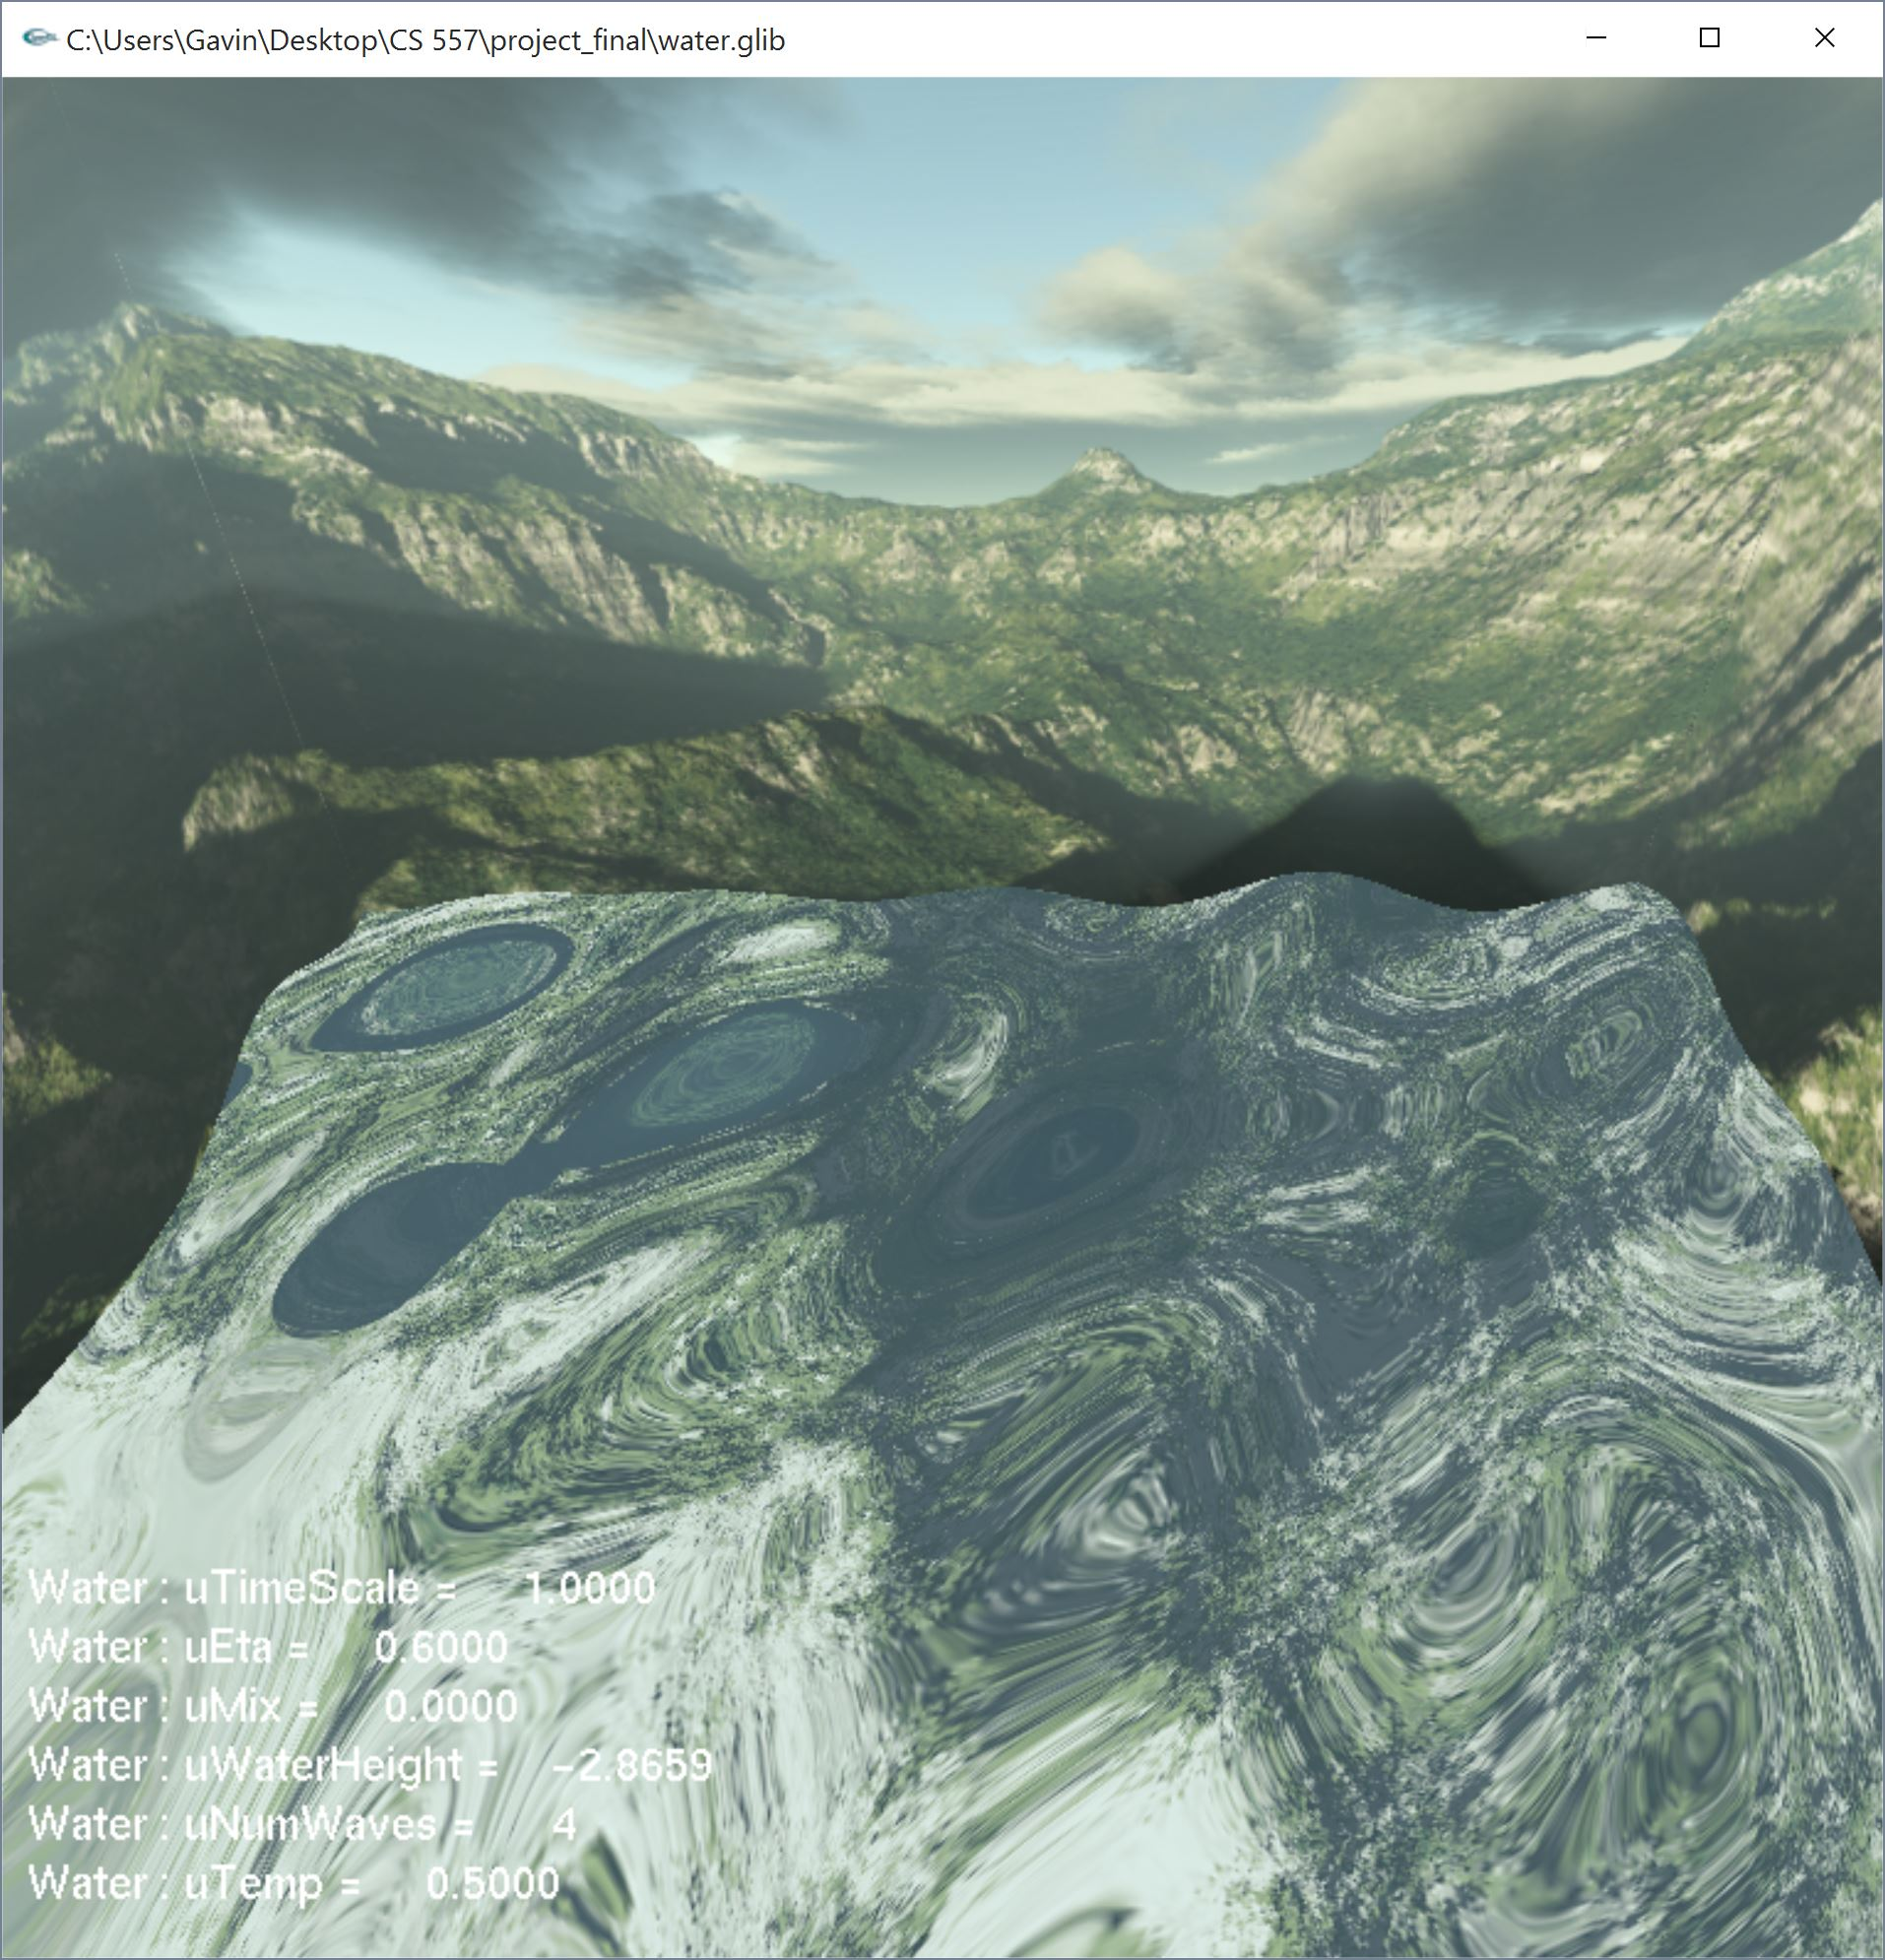
\includegraphics[width=2.9in]{refr.jpg}
	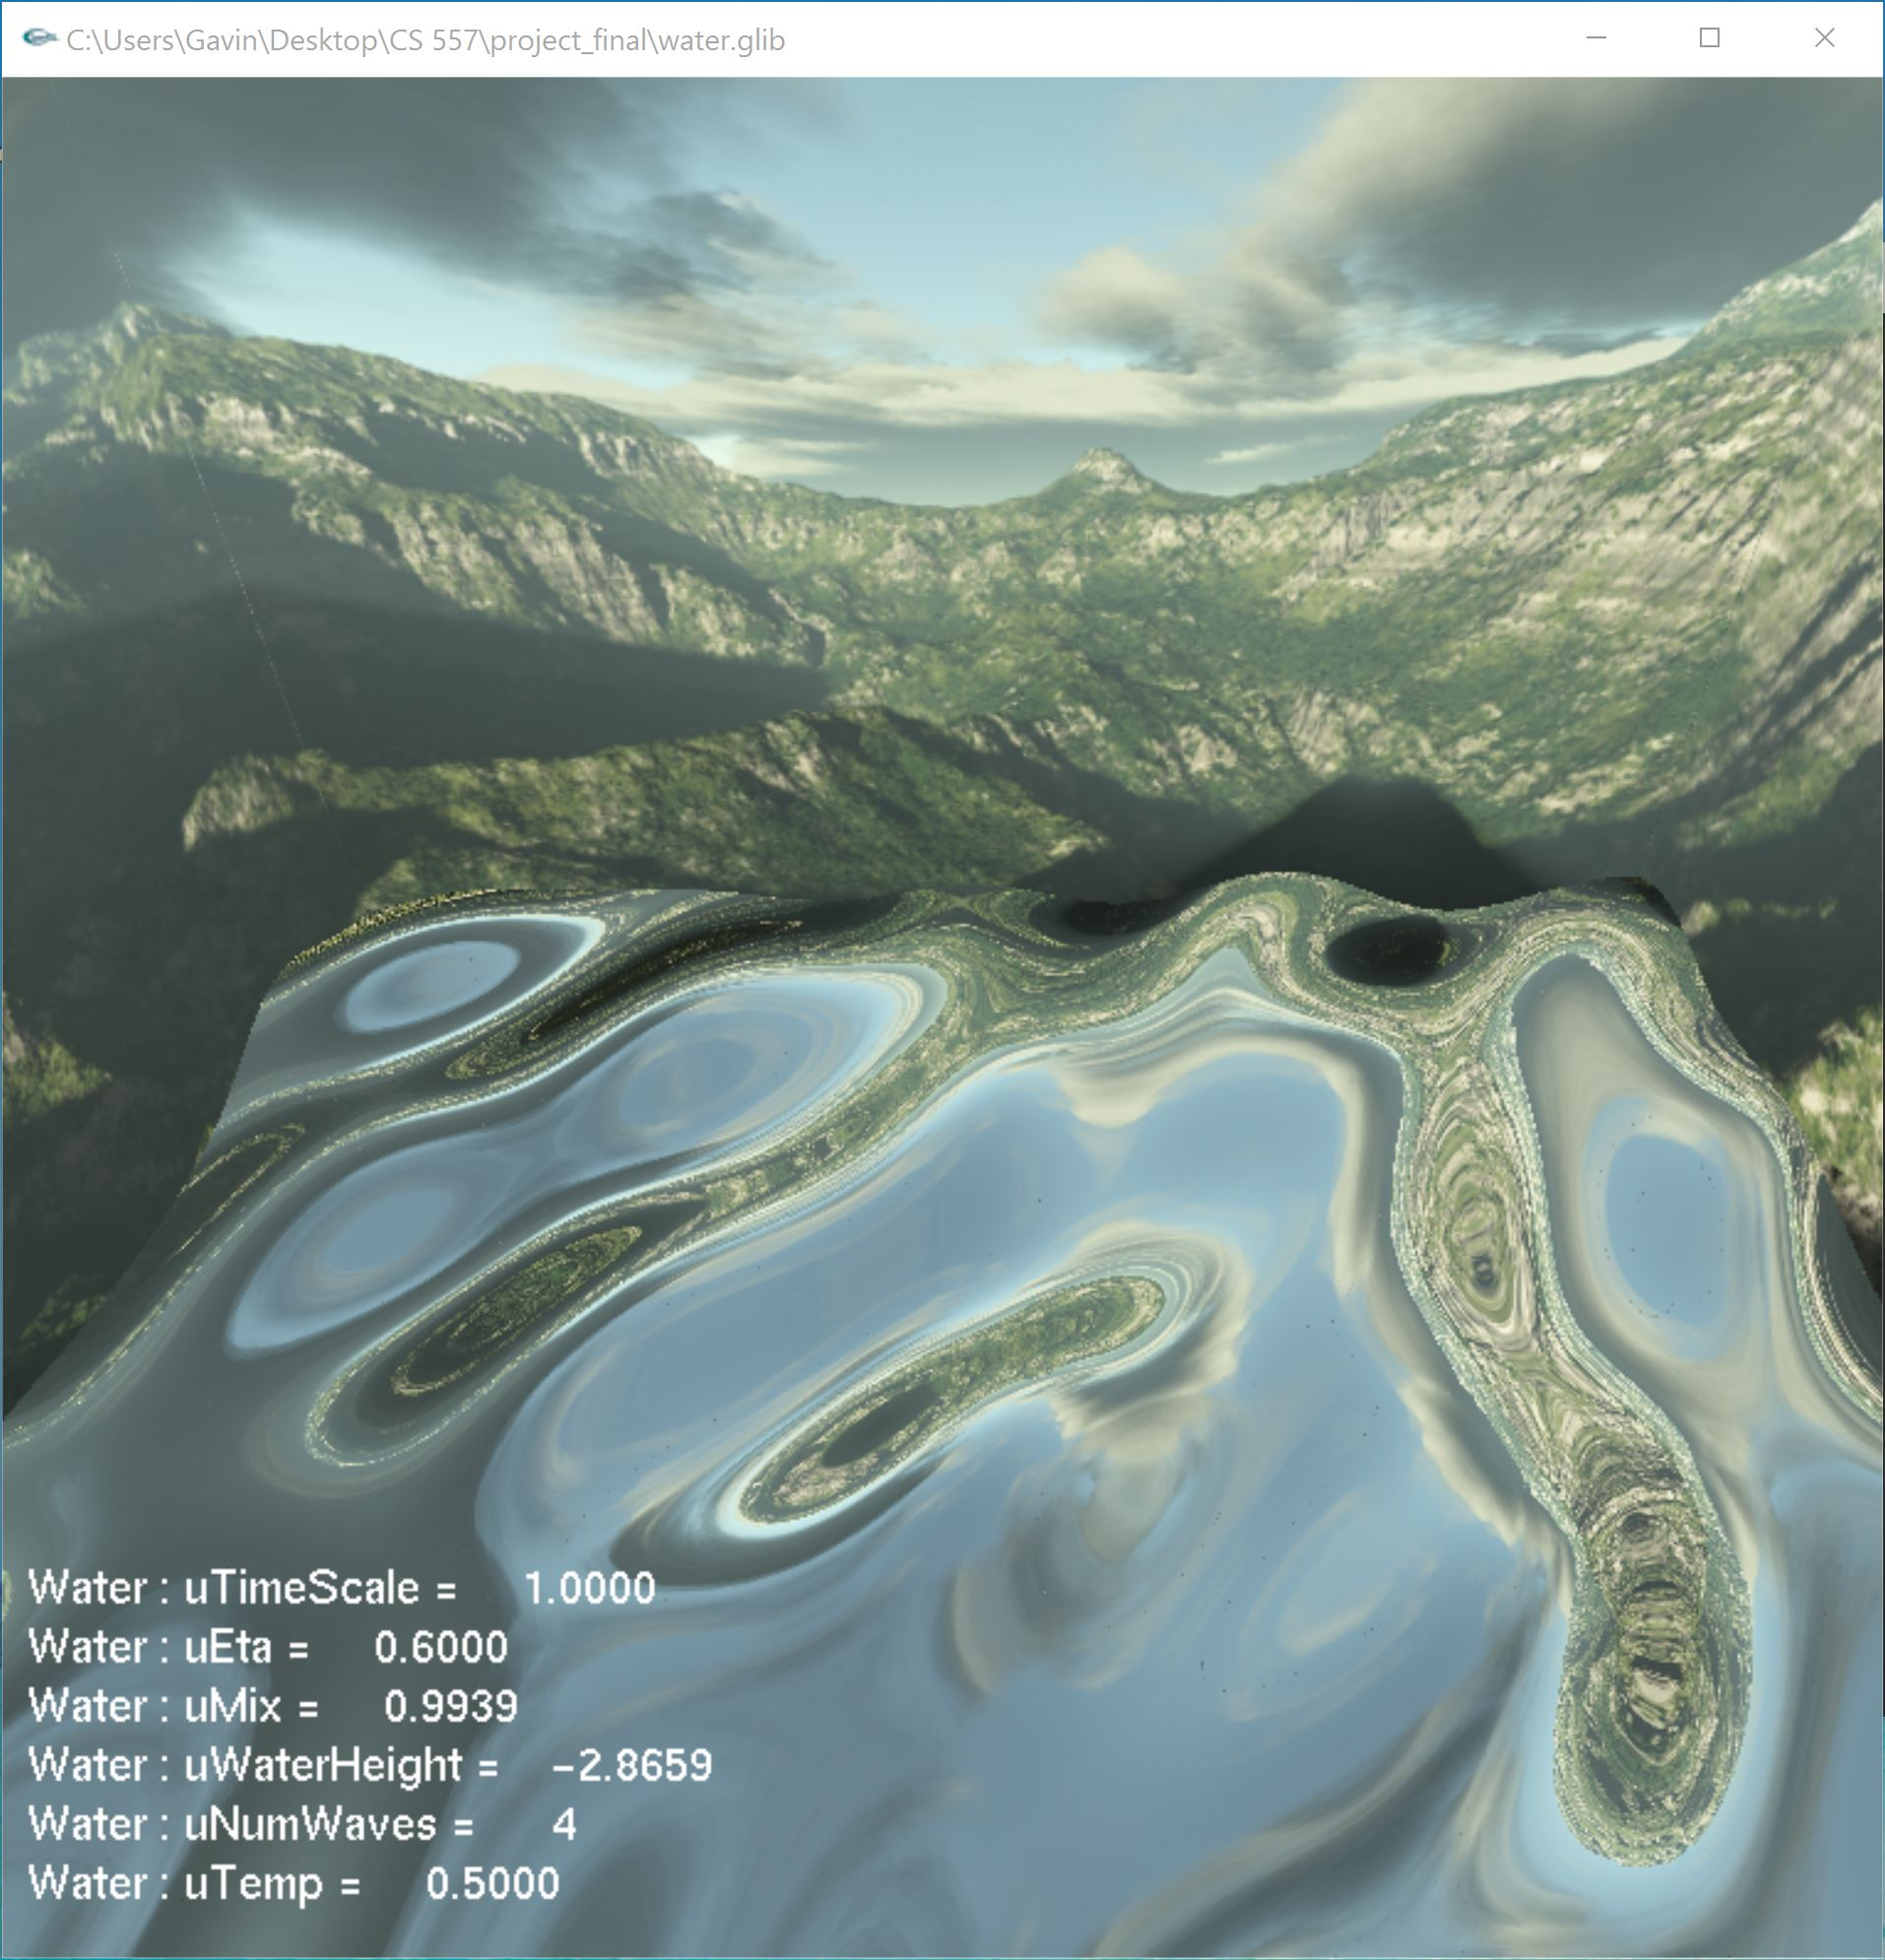
\includegraphics[width=2.9in]{refl.jpg}
\end{center}
The Eta value controlled by the uEta slider is the coefficient of the refraction. By changing the its value the pattern refracted by the water surface will be changed. The following image shows the effect by changing the eta value. The original value is set to 0.6, and the eta in the image is set to less than 0.2. Comparing with the pattern in the image at above left, the difference chould be told.
\begin{center}
	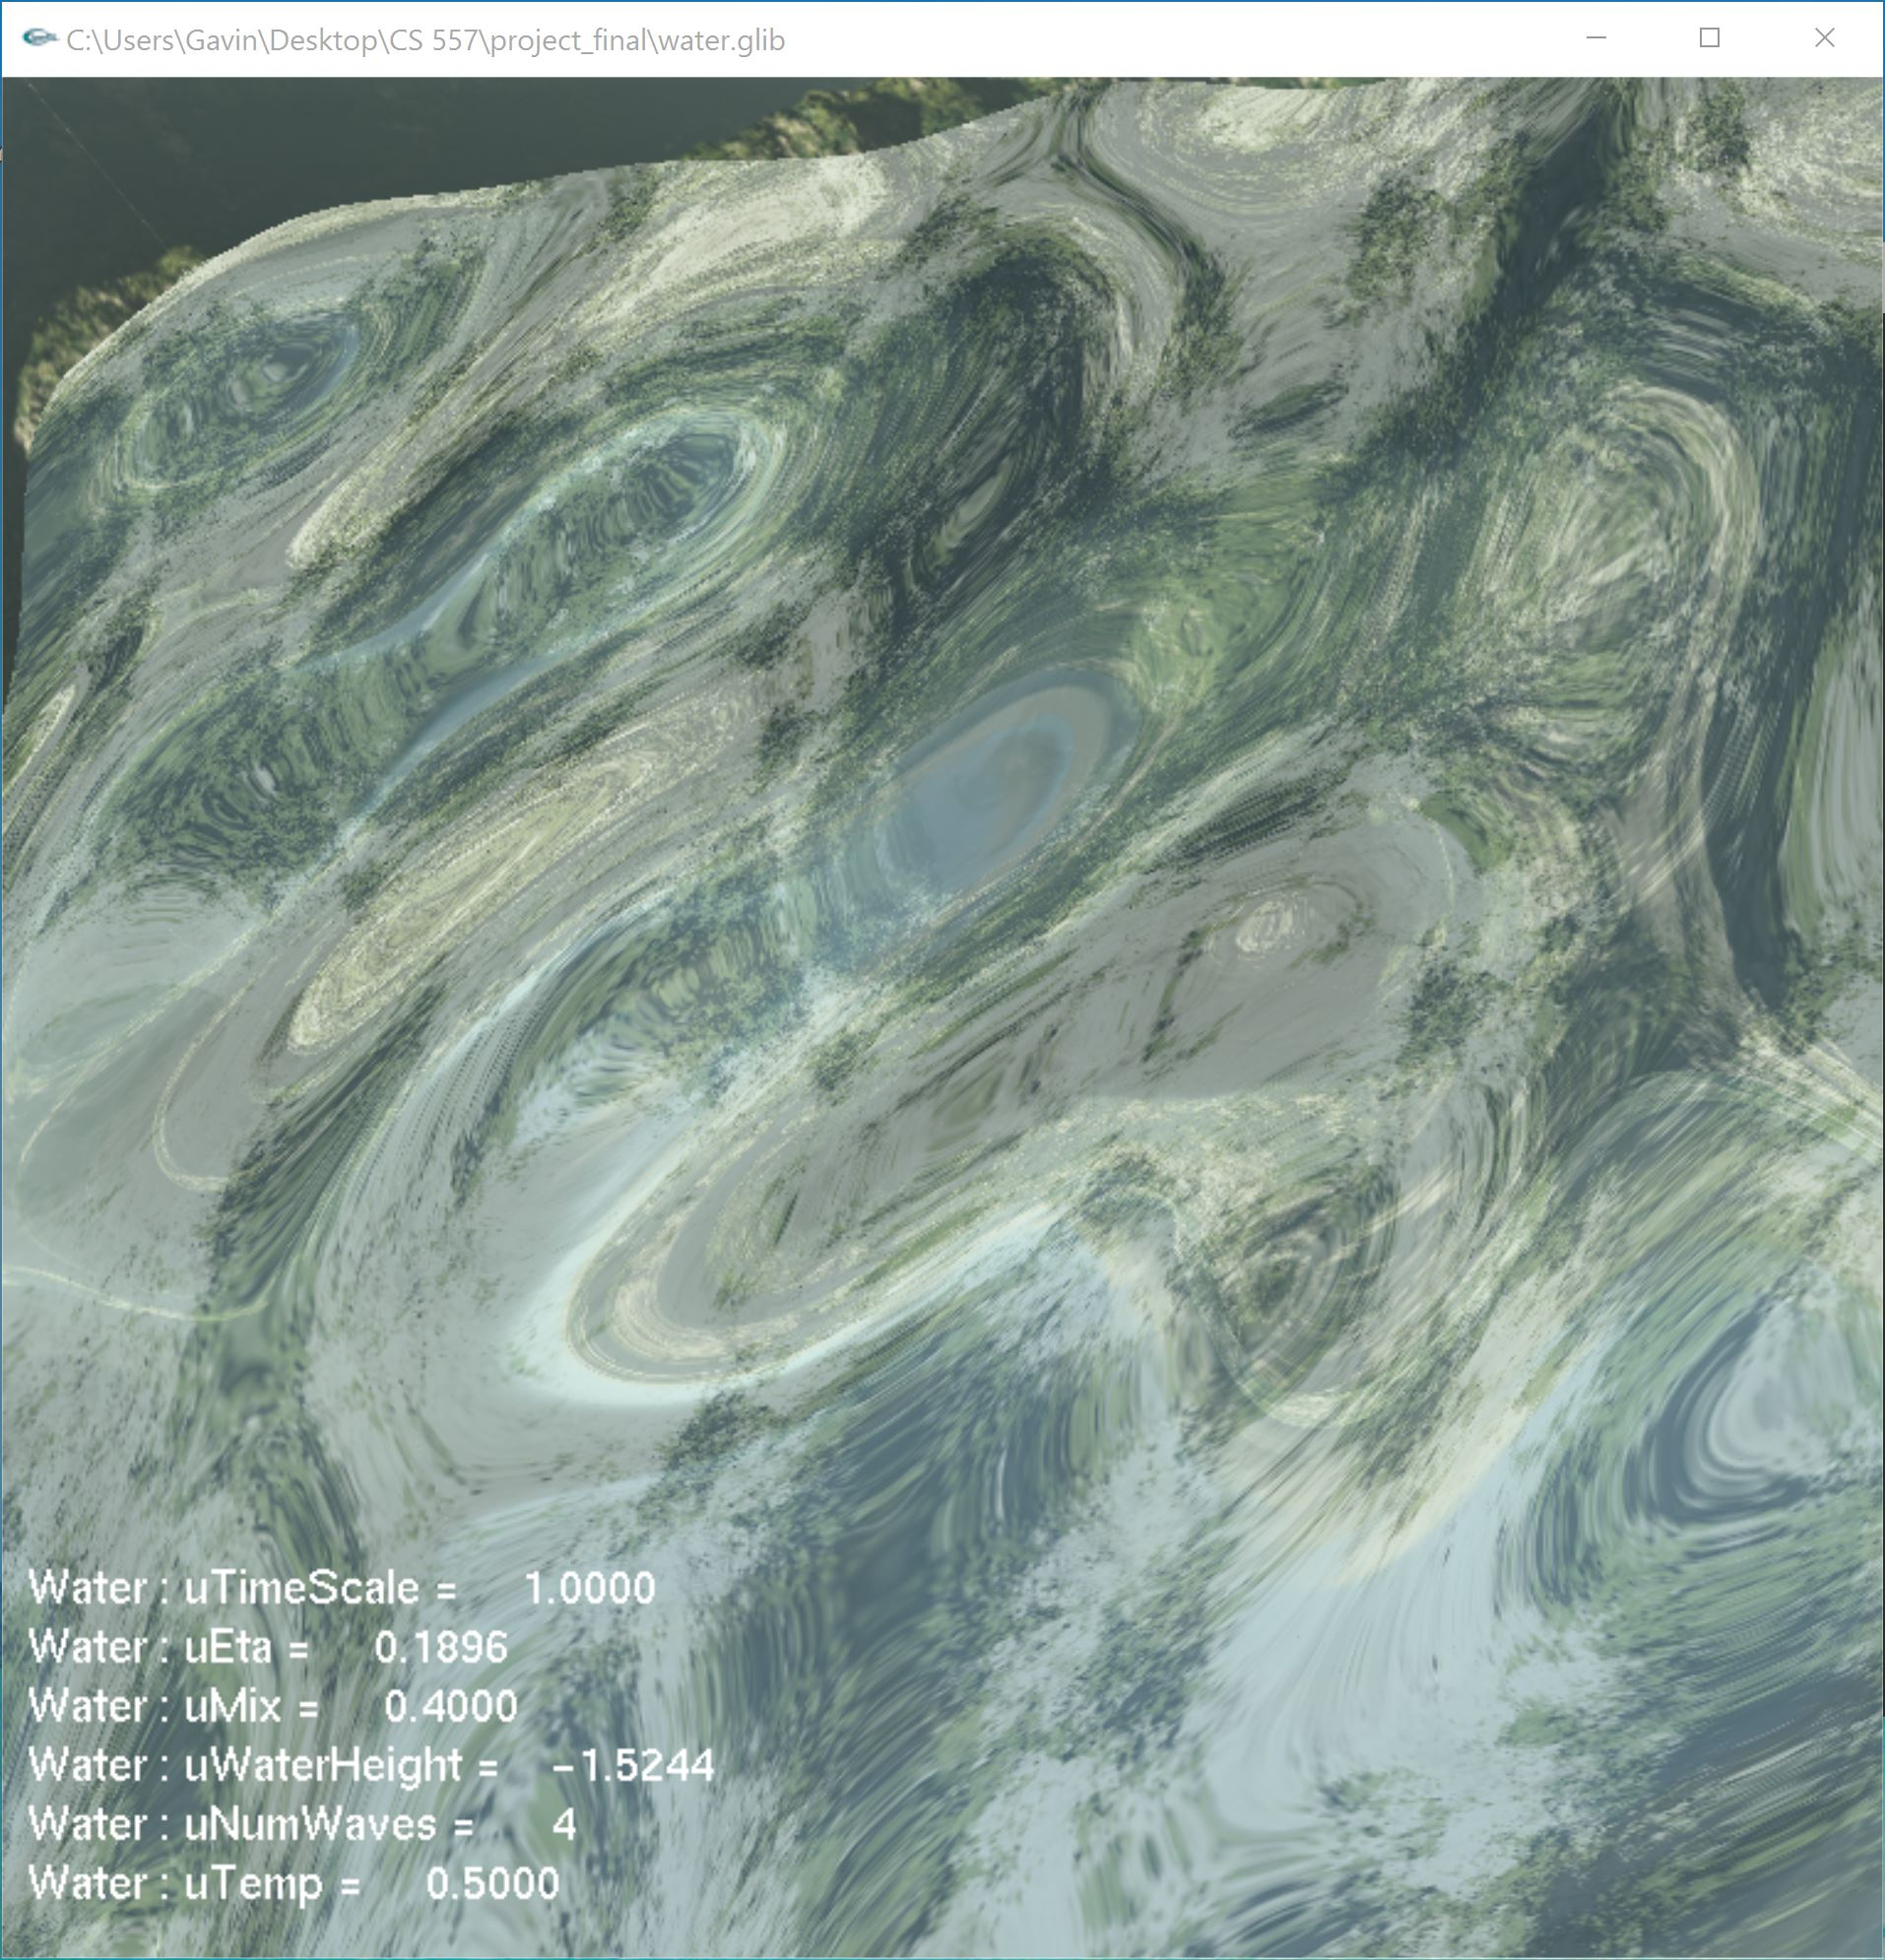
\includegraphics[width=2.9in]{eta.jpg}
\end{center}
Excepting the original water surface implementation, the morphological changes are also implemented into this program. By changing the temperature with the uTemp slider, the water will become ether ice or cloud. The range of the slider is set to $[-1, 2]$ since the real range of temperature is too large to handle. In the range $(0, 1)$, the water remains in fluid form, and this range is the part that the original water simulation works. In the range $[-1, 0]$ the water won't move anymore and becomes ice. 

In this range, the lower temperature is the whiter ice becomes. This is done by setting a range of y values relates to uTemp. For the fragments on the surface above the y value, a tested ice color ($ICECOLOR = vec3( 0.75, 0.85, 1.)$) will be mixed into its fragment color. The edge of the ``whit line'' is blurred using tolerance and smoothstep. In order to create the ``rugged'' surface of the ice, bump mapping is used with the noise to turn the normals with an random angle. Further, the eta value is also automatic changed to perform the different refraction coefficient between ice and water. The following 2 images show different ice effects with different temperature values.
\begin{center}
	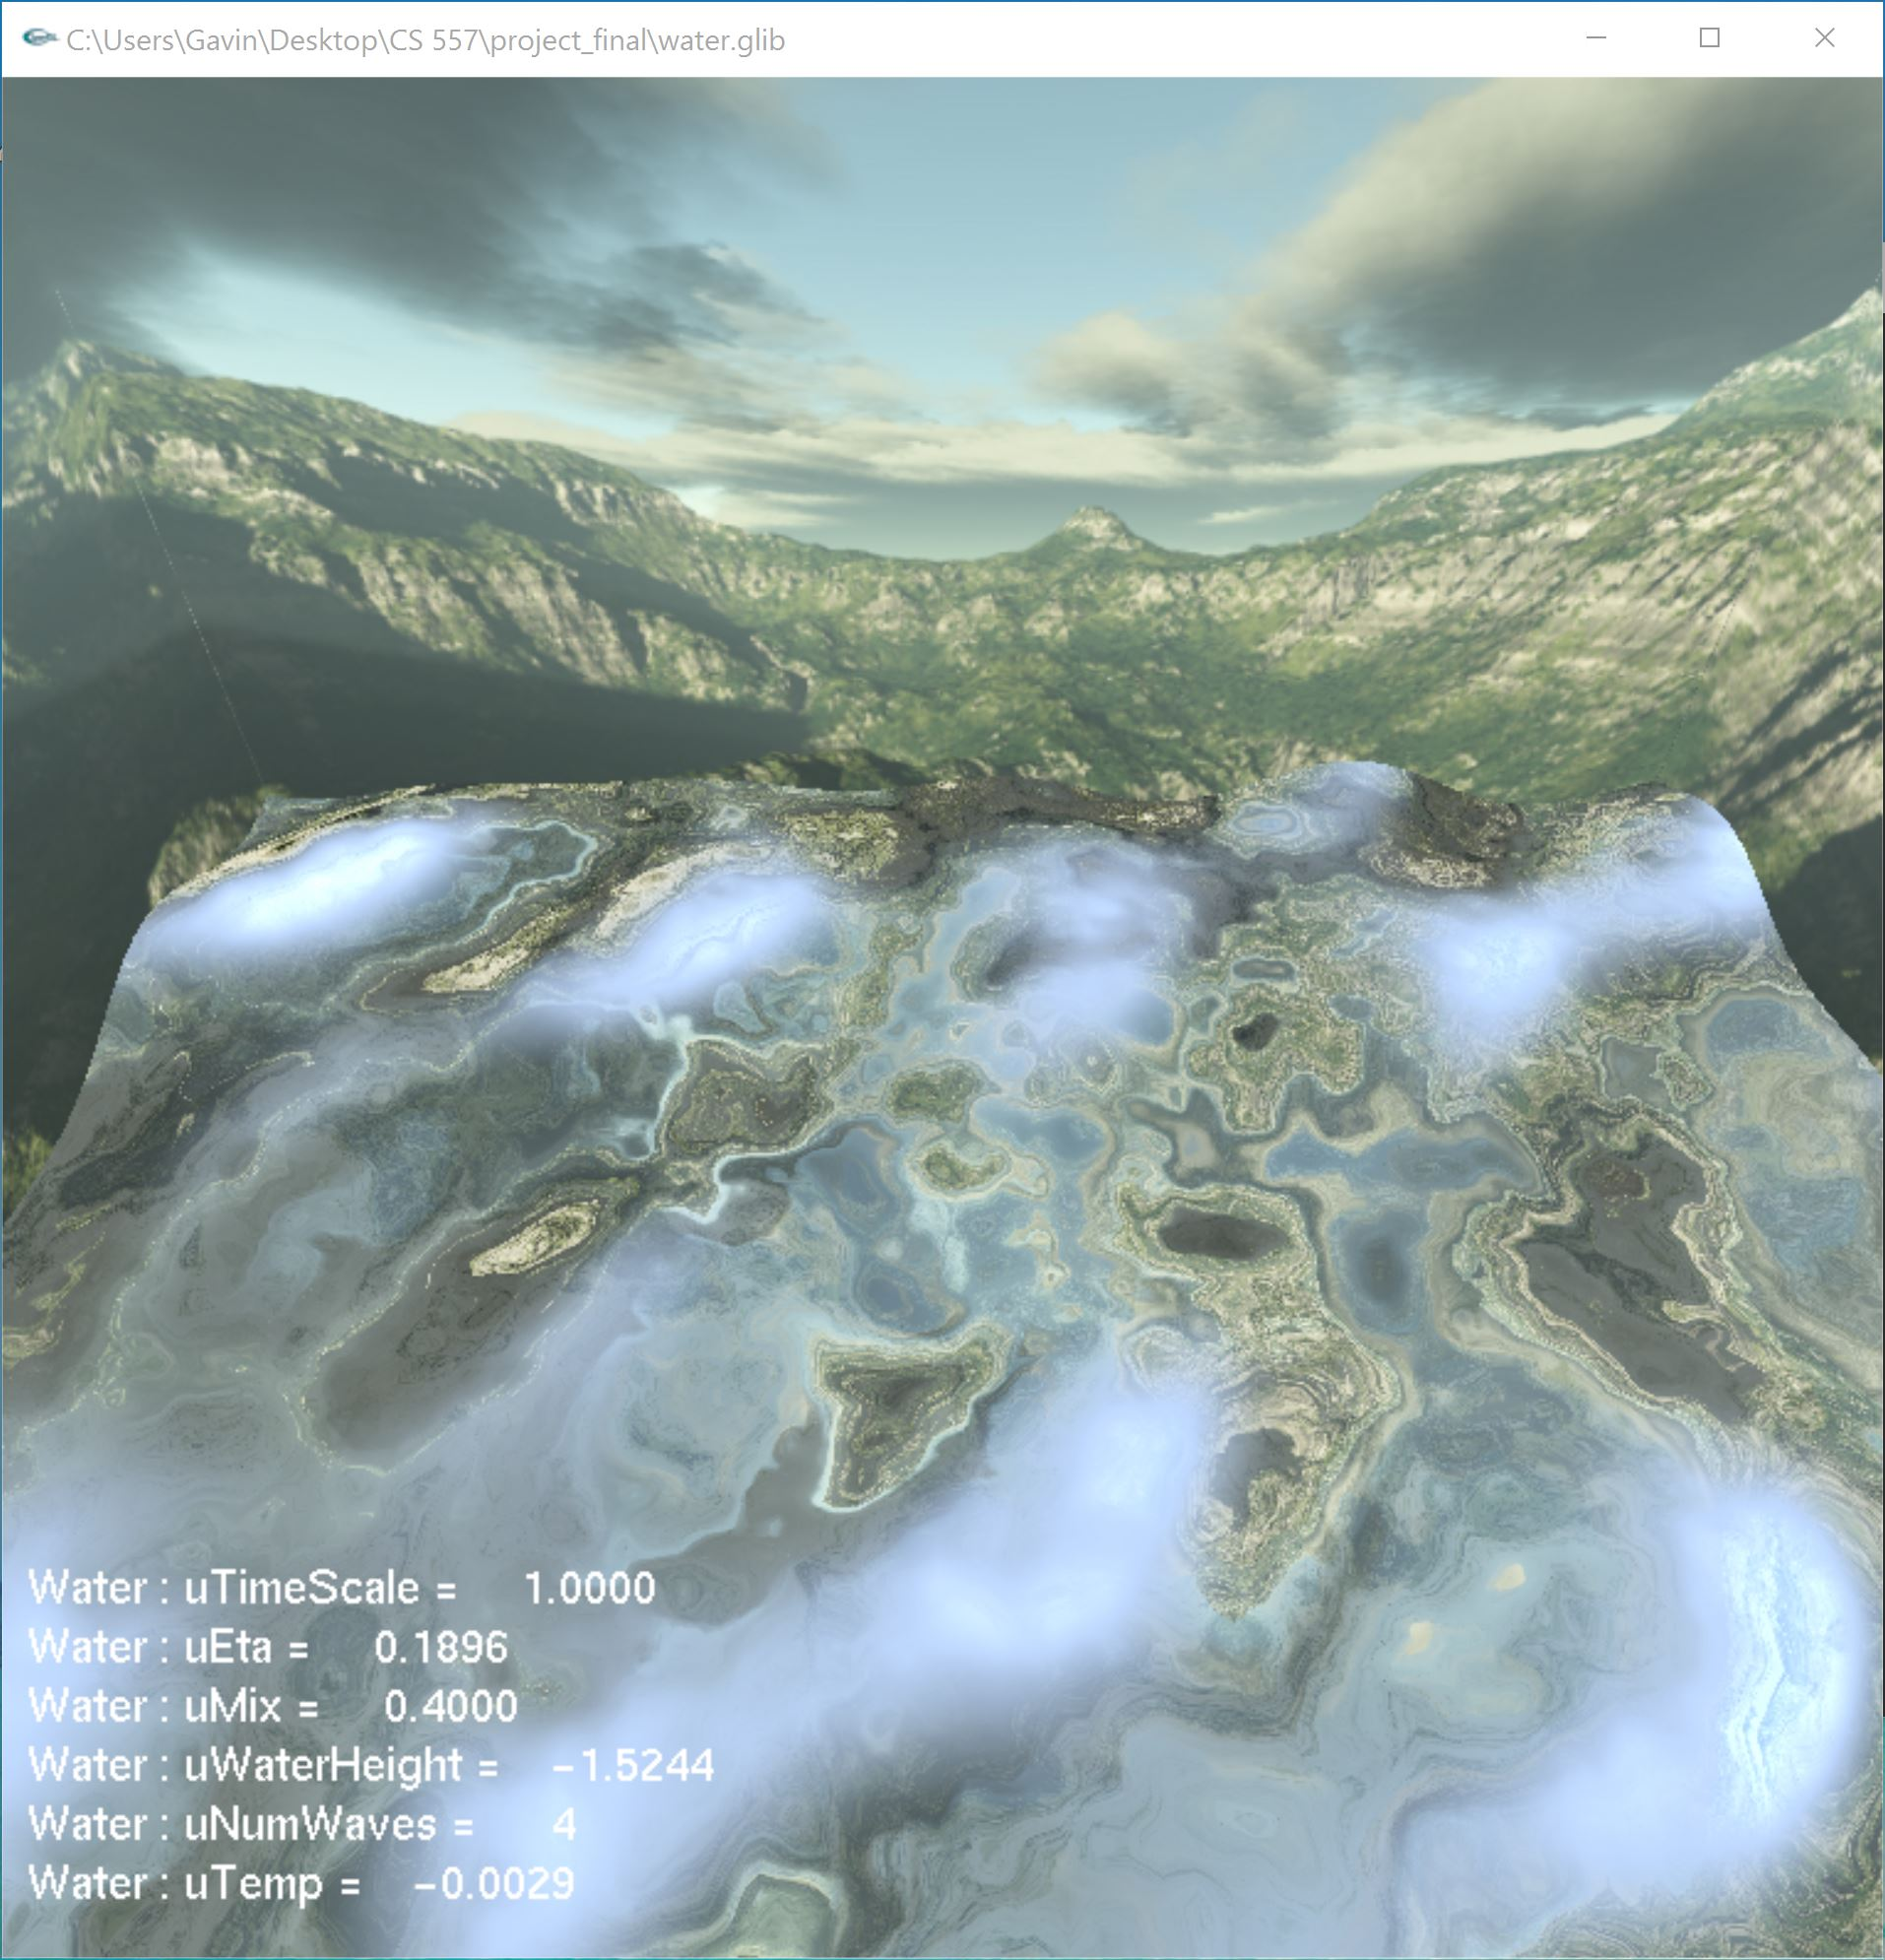
\includegraphics[width=2.8in]{ice1.jpg}
	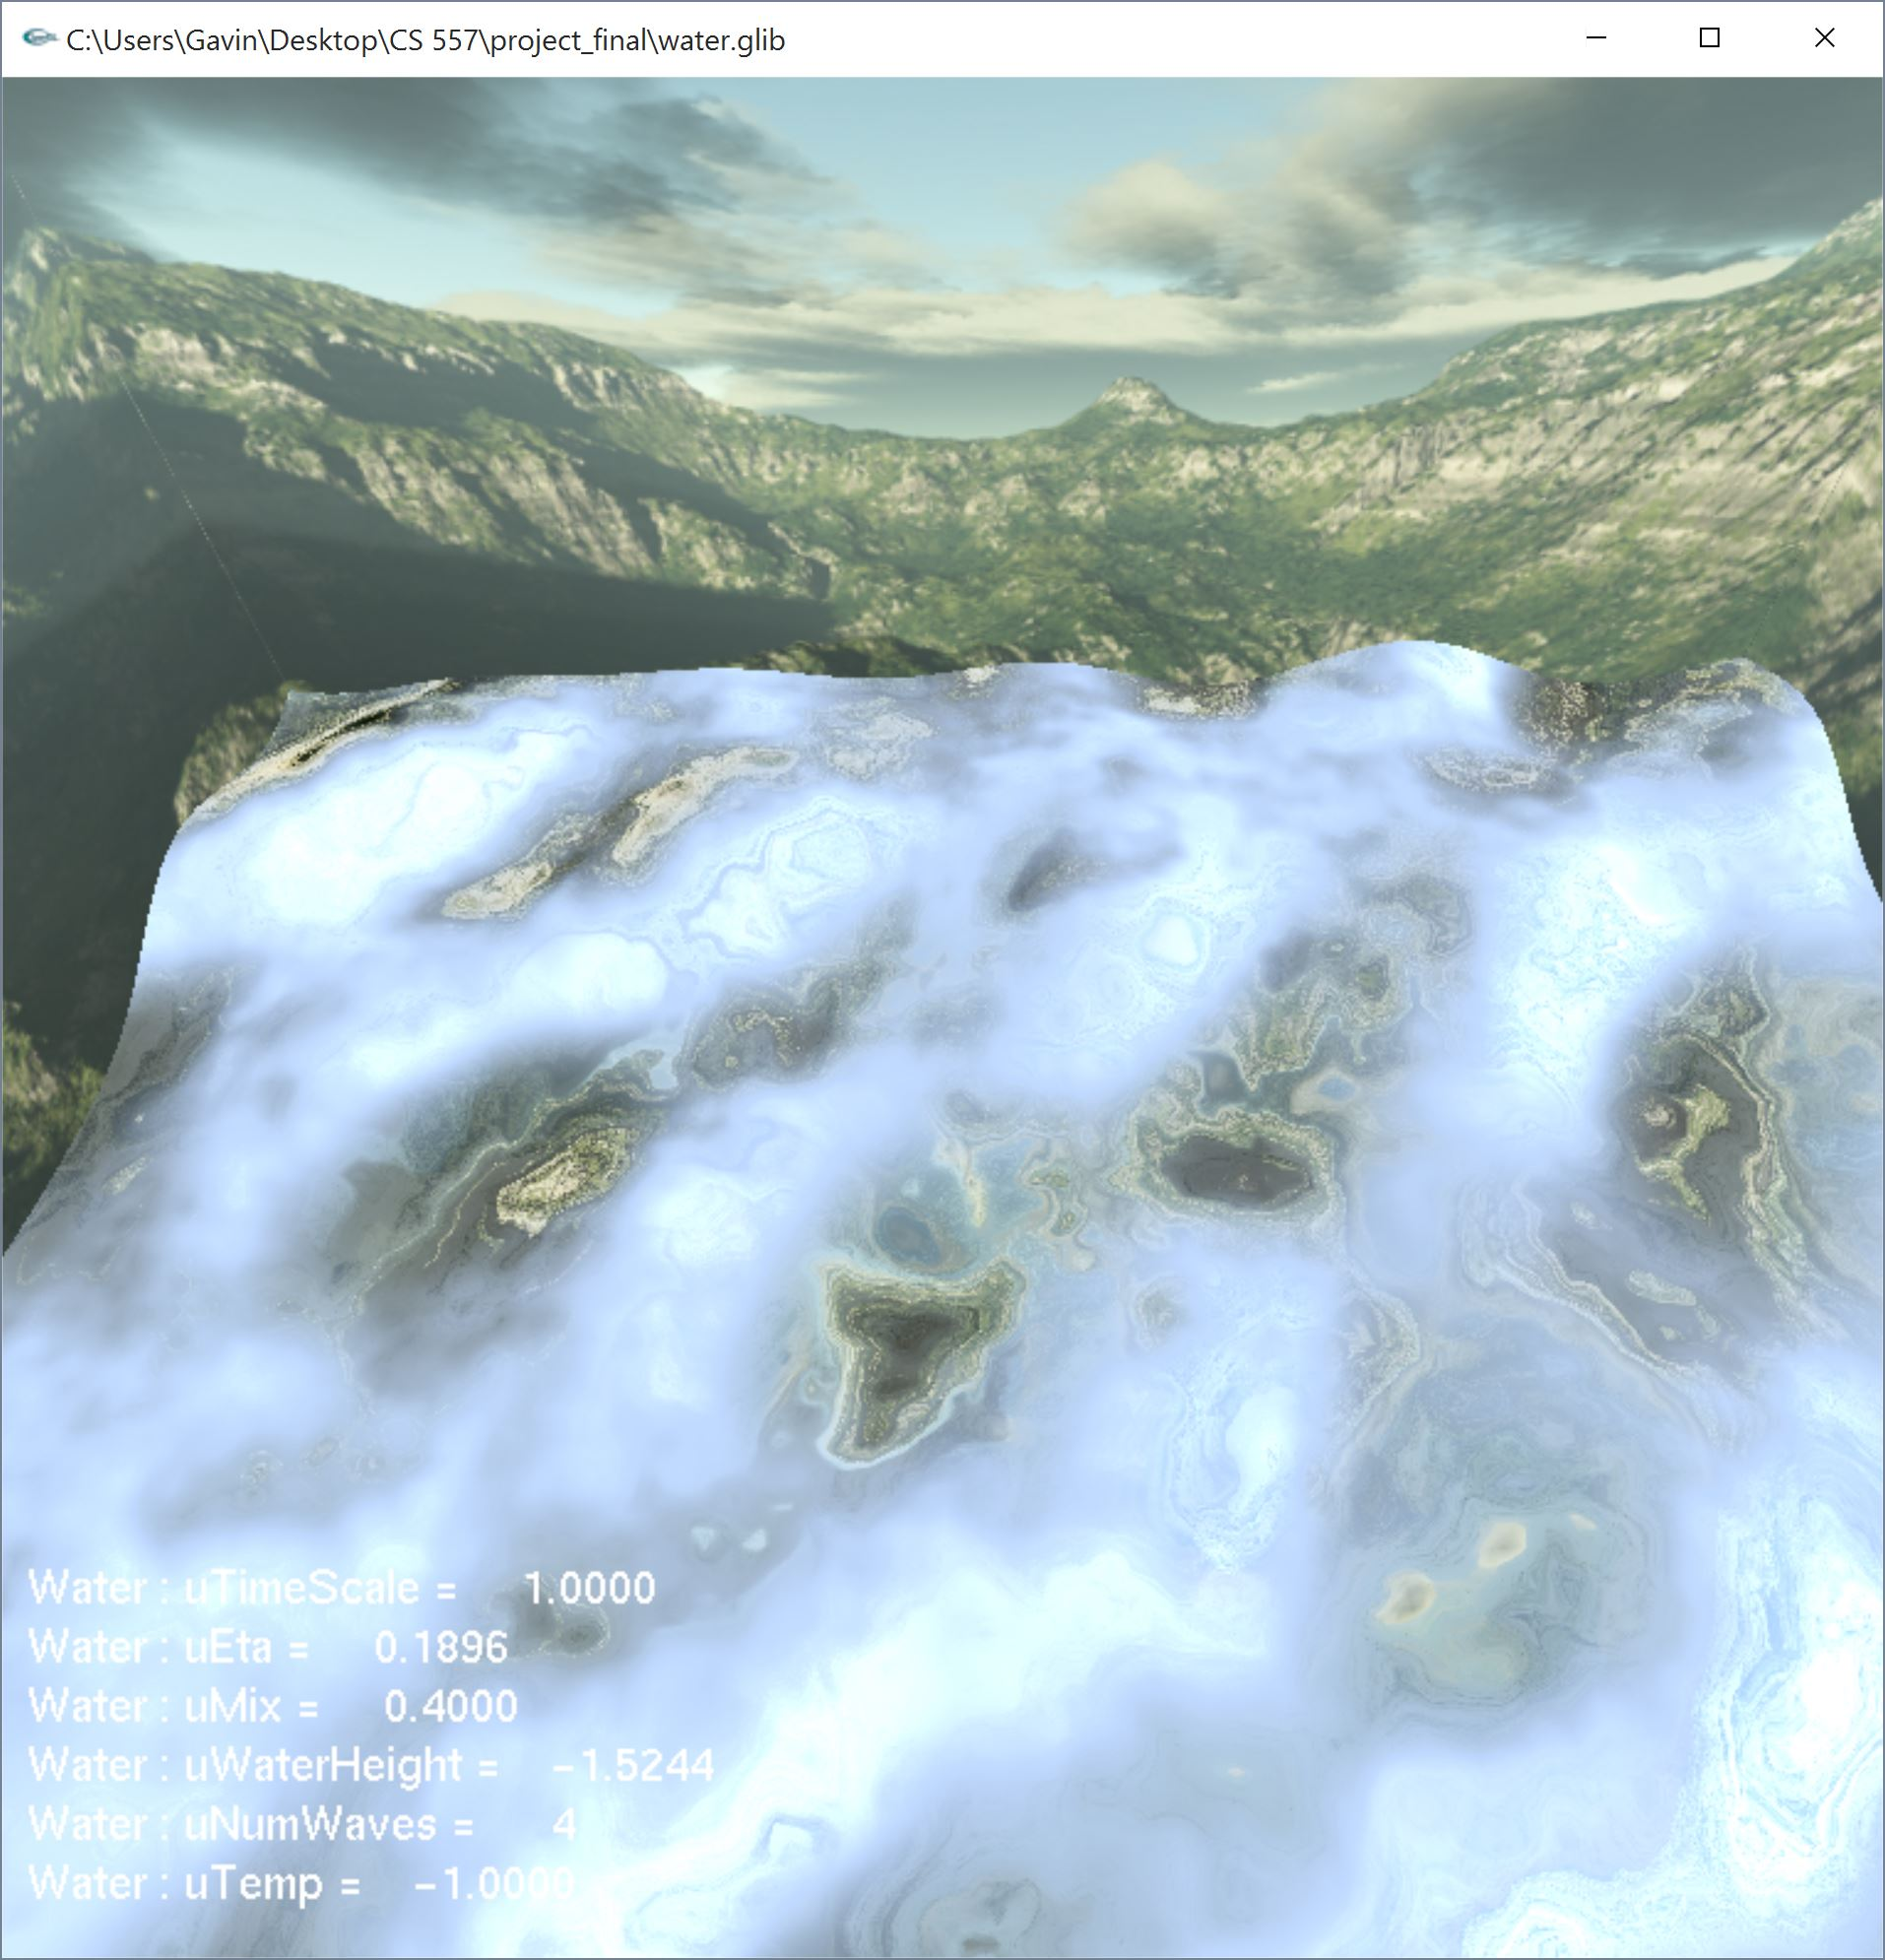
\includegraphics[width=2.8in]{ice2.jpg}
\end{center}
In the range $[1, 2]$, the water will be evaporated into cloud. The cloud in this project is not the dynamic volume cloud but a pattern lies on the surface. By changing the color and opacity on the water plane, a ``cloud-like'' pattern will be created. The idea of drawing clouds is similar to drawing ``white ice'', the difference is the white intensity for the cloud color and its opacity come from the normal at that fragment. By adding up the three components of the normal, a scaler value will be produced. Multiply this scaler value to white color will result to the fragment color, and the scaler value itself could be the opacity. When the scaler value is less than 0, it will be set to 0. The result of these steps shows up pretty good. The density of the cloud is also connected tot he temperature, the higher temperature is, the more density the cloud has. The following 2 images shows the effect with different temperature. 
\begin{center}
	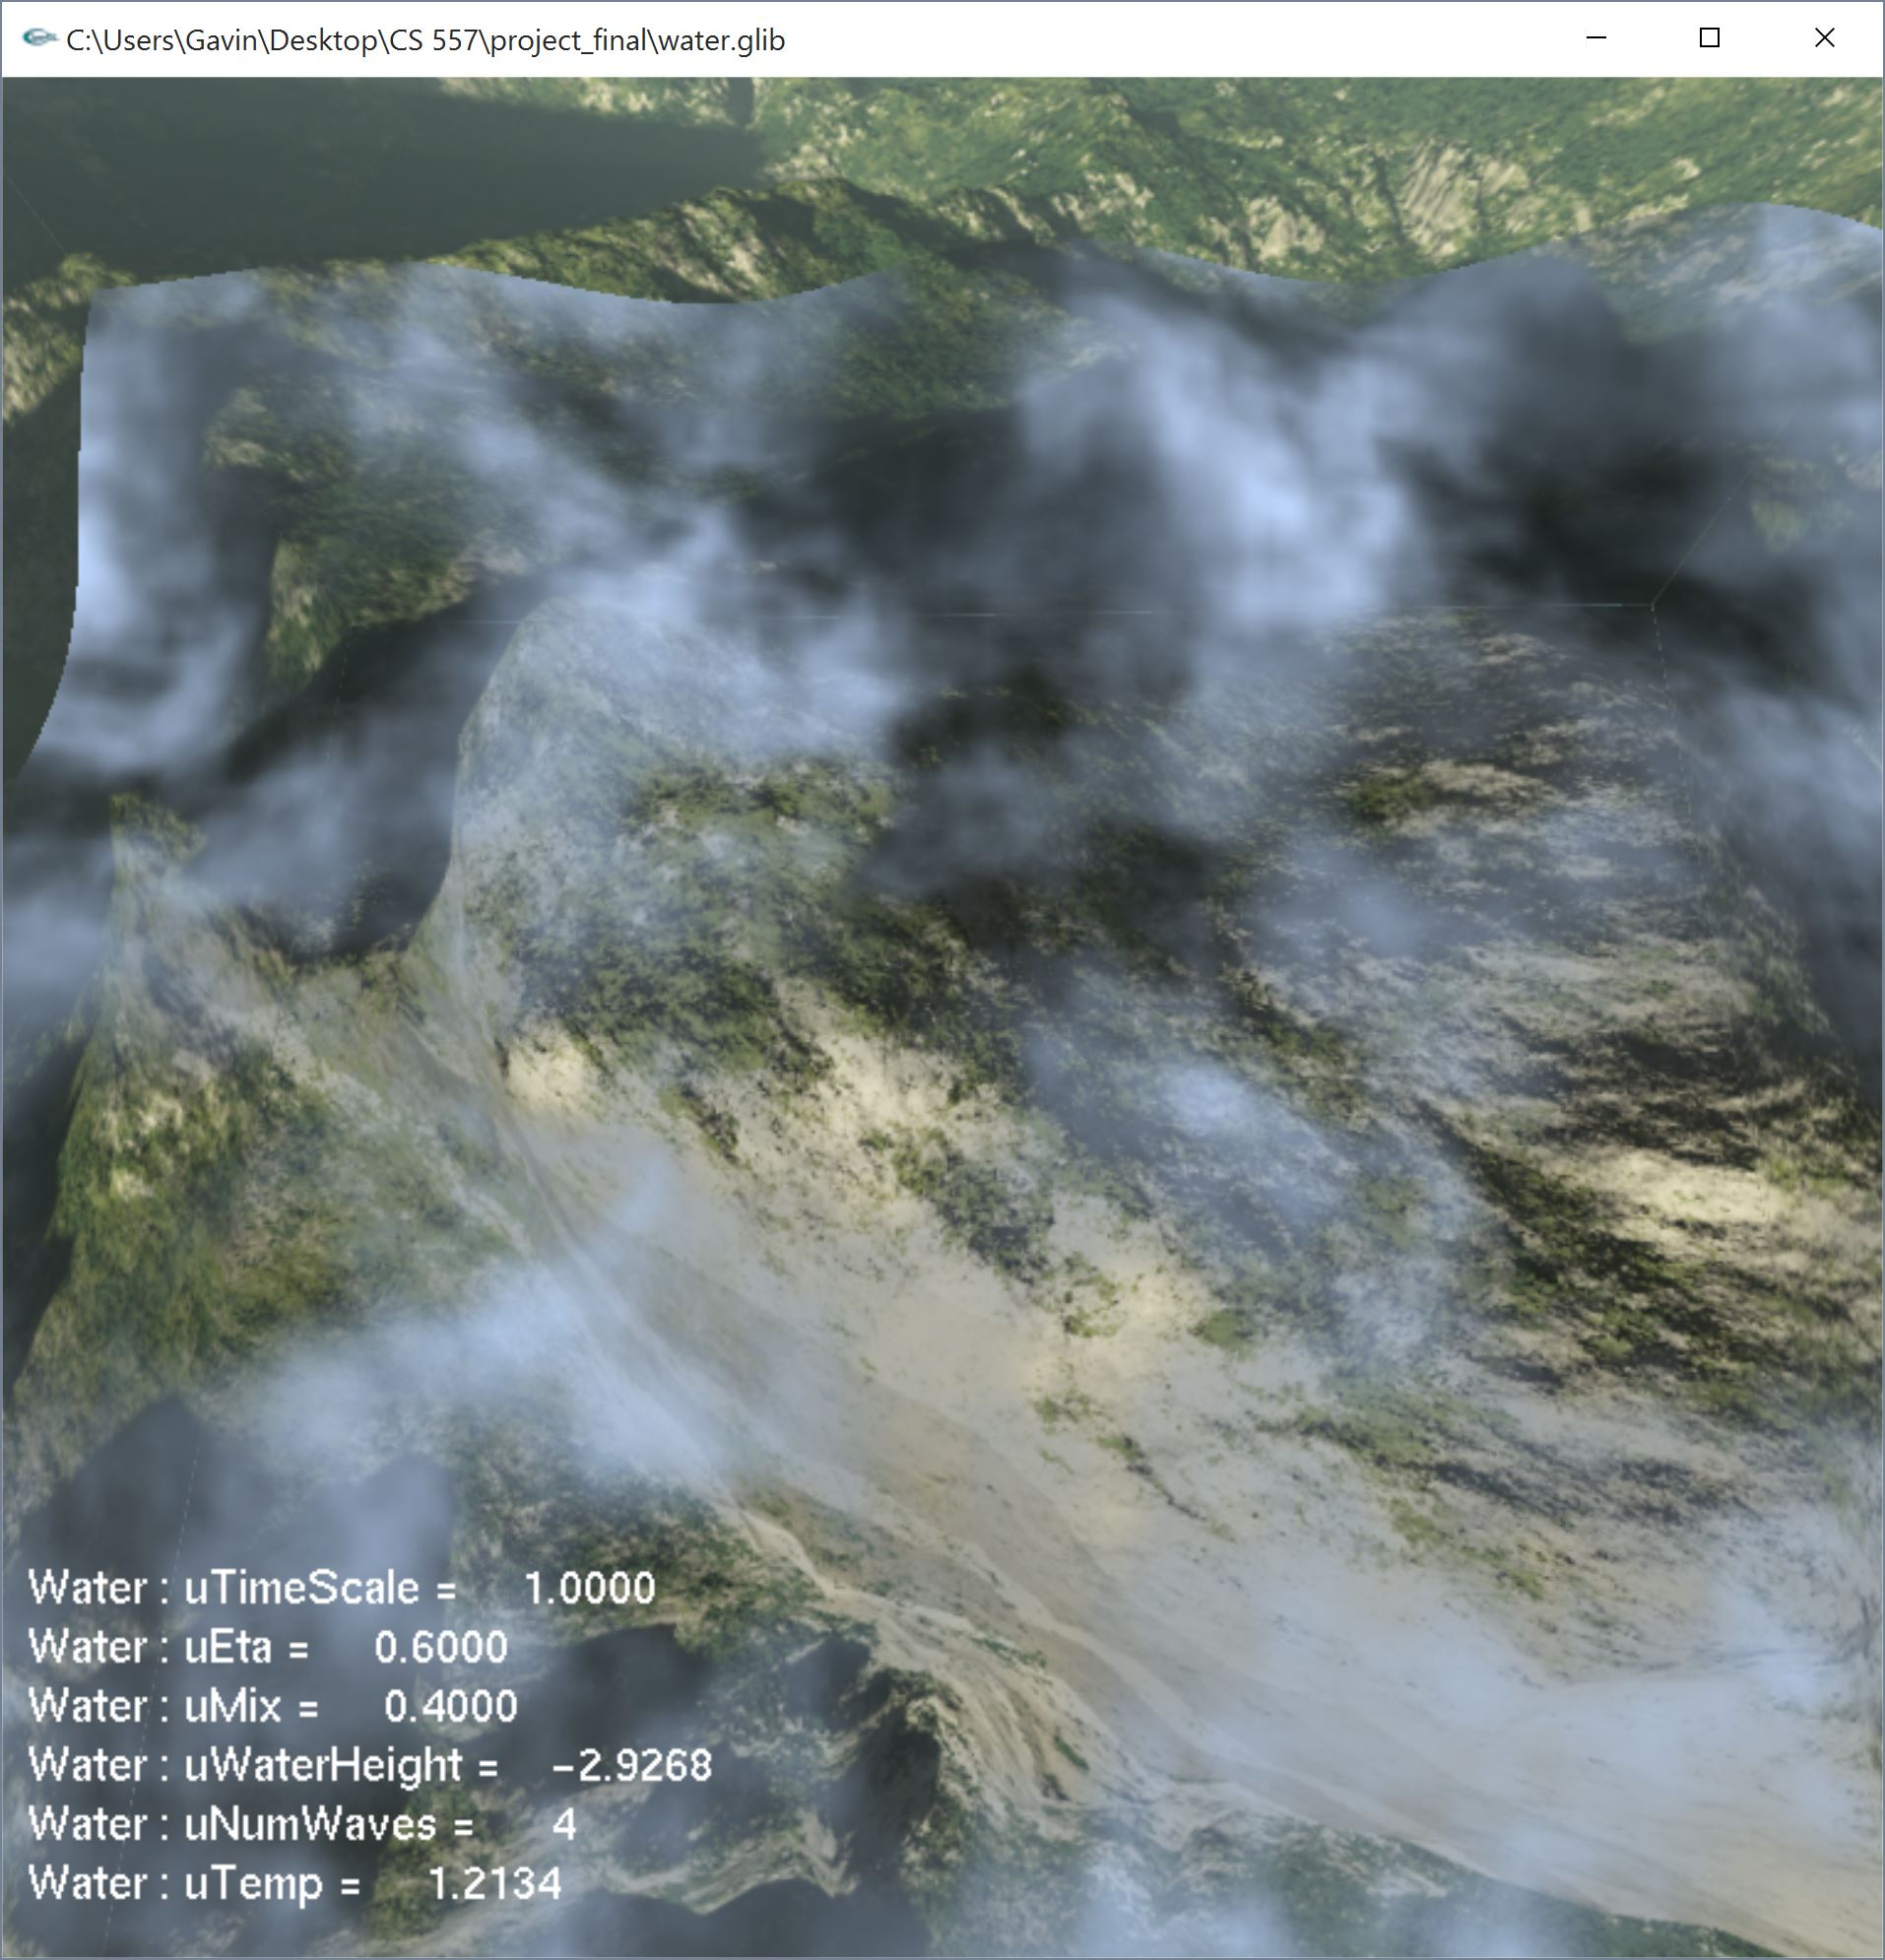
\includegraphics[width=2.8in]{cloud1.jpg}
	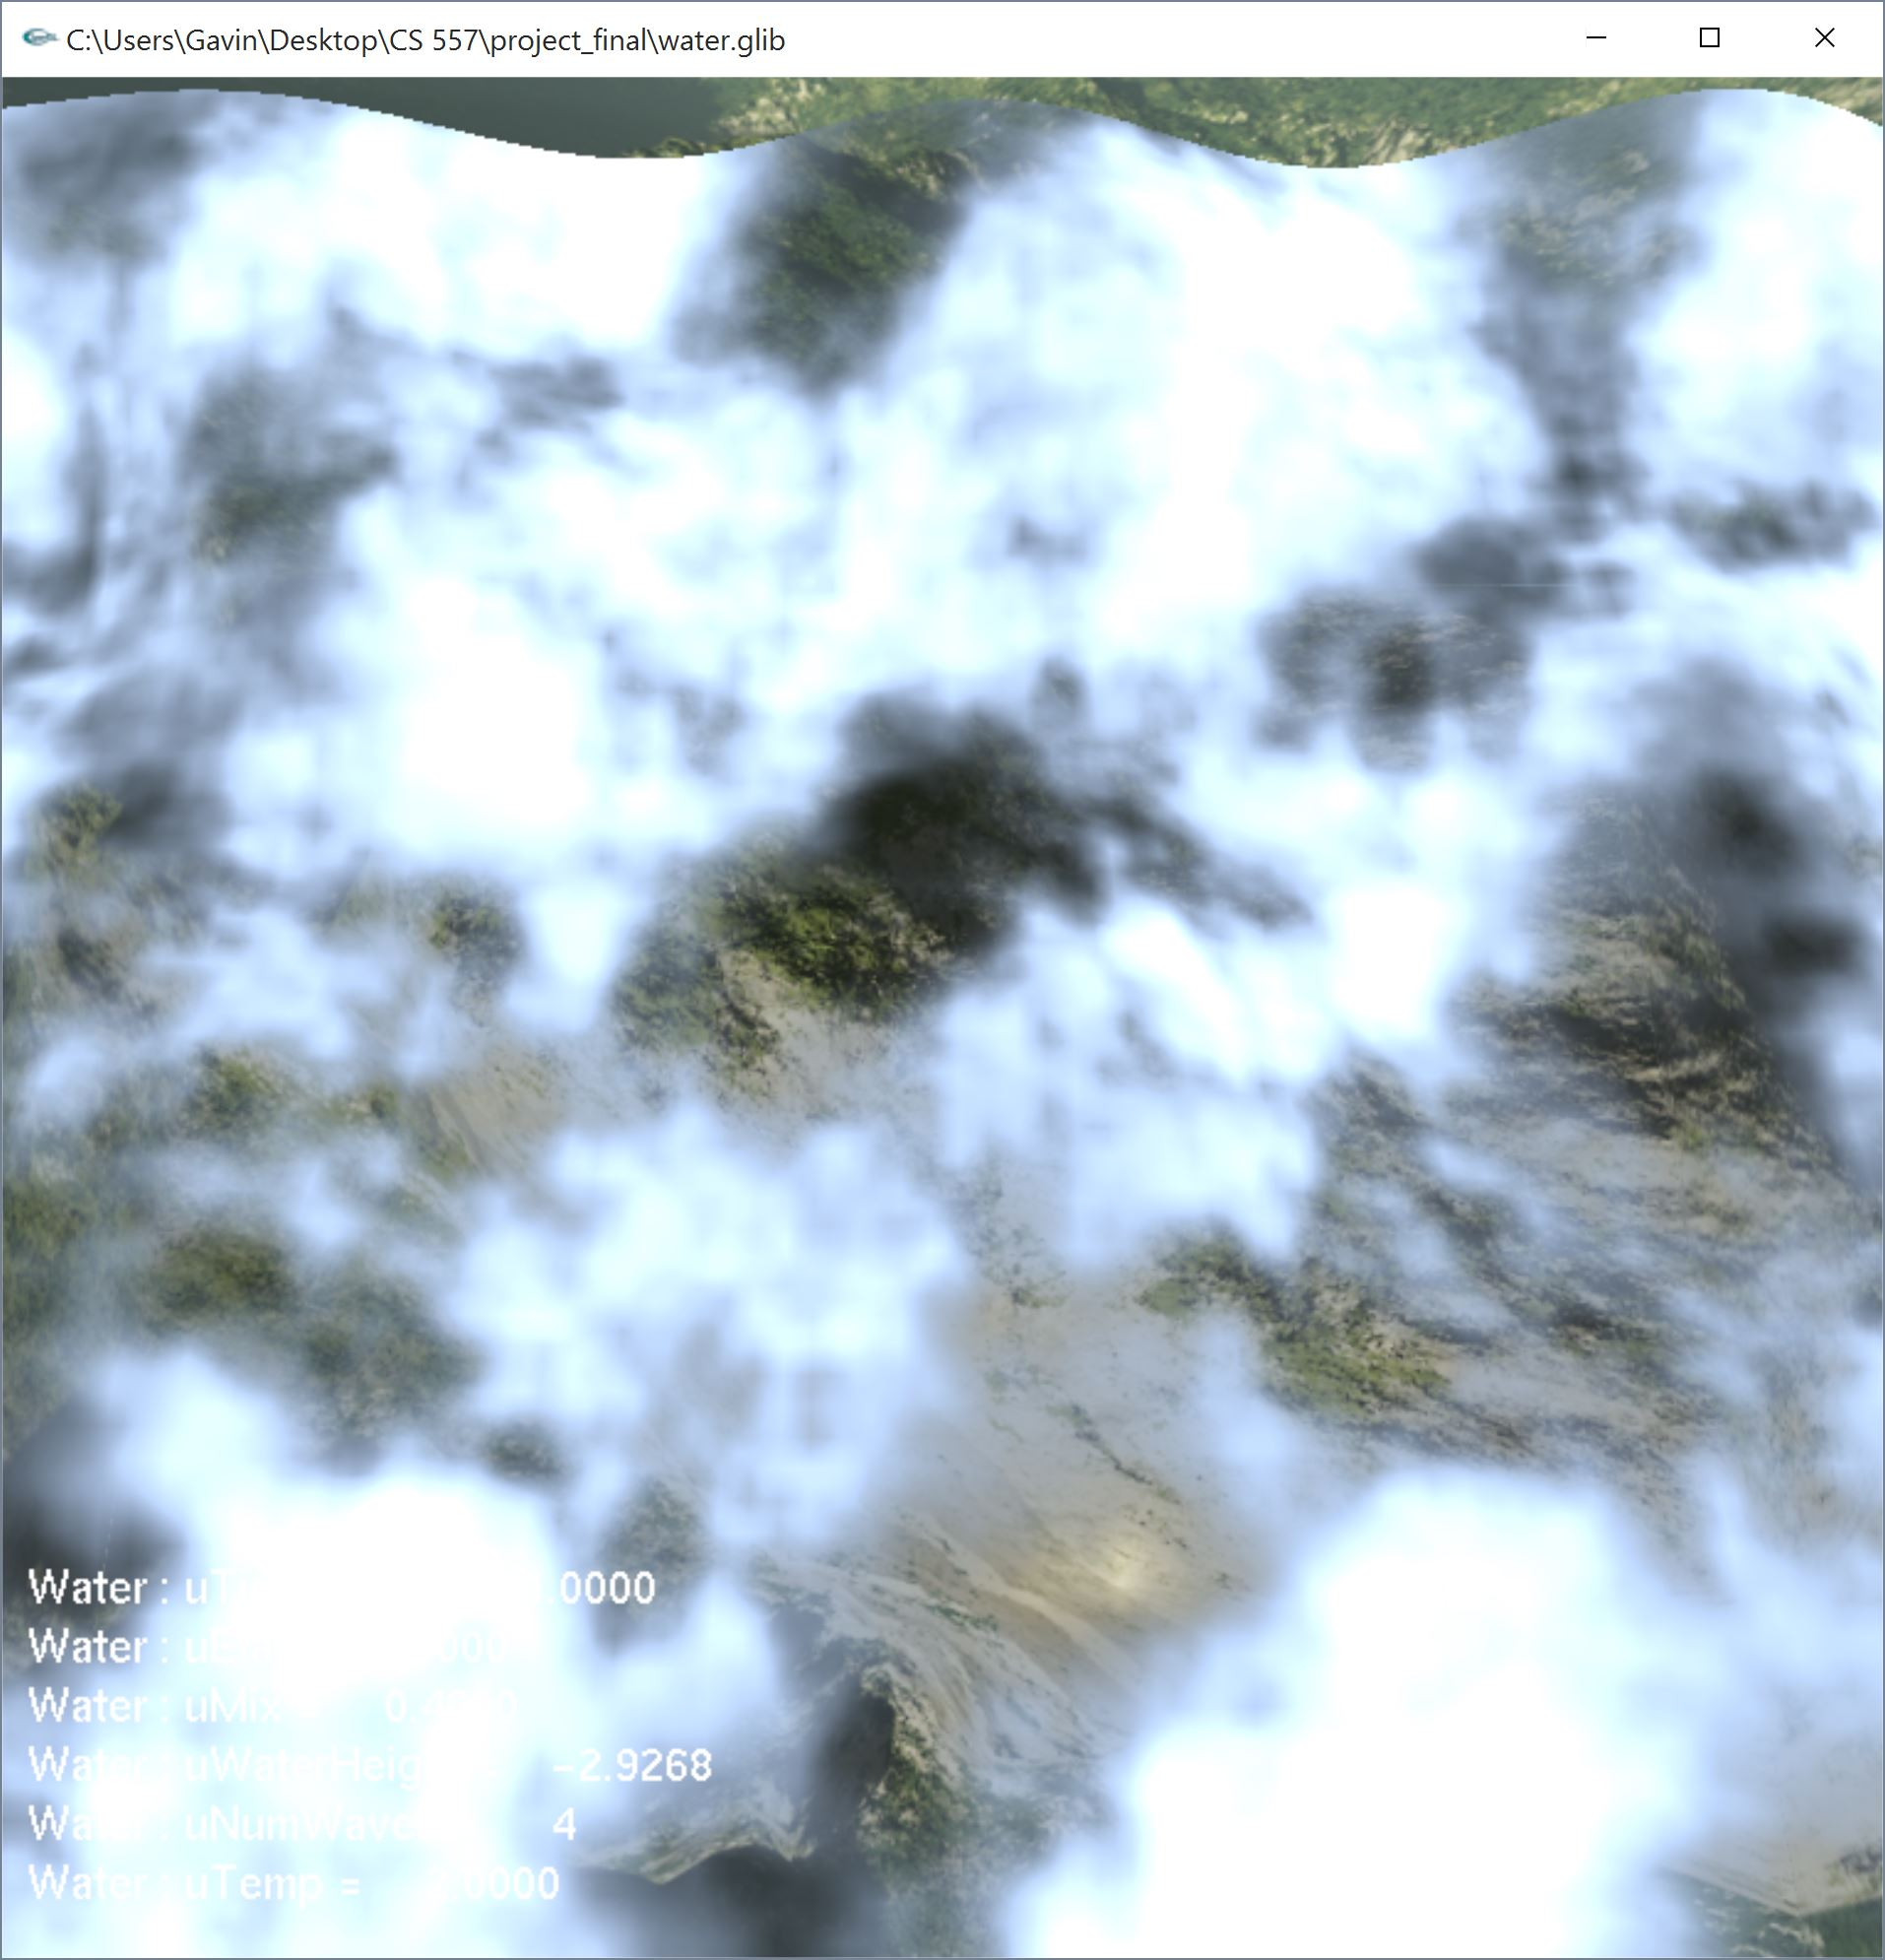
\includegraphics[width=2.8in]{cloud2.jpg}
\end{center}
The height of the cloud is also connected to the temperature. The higher the pemperature is, the higher the cloud moves. The following three images show the different height of the water surface and the cloud. These three images are taken from exactly same position and view direction, and the red line in the image shows the height of the surface.
\begin{center}
	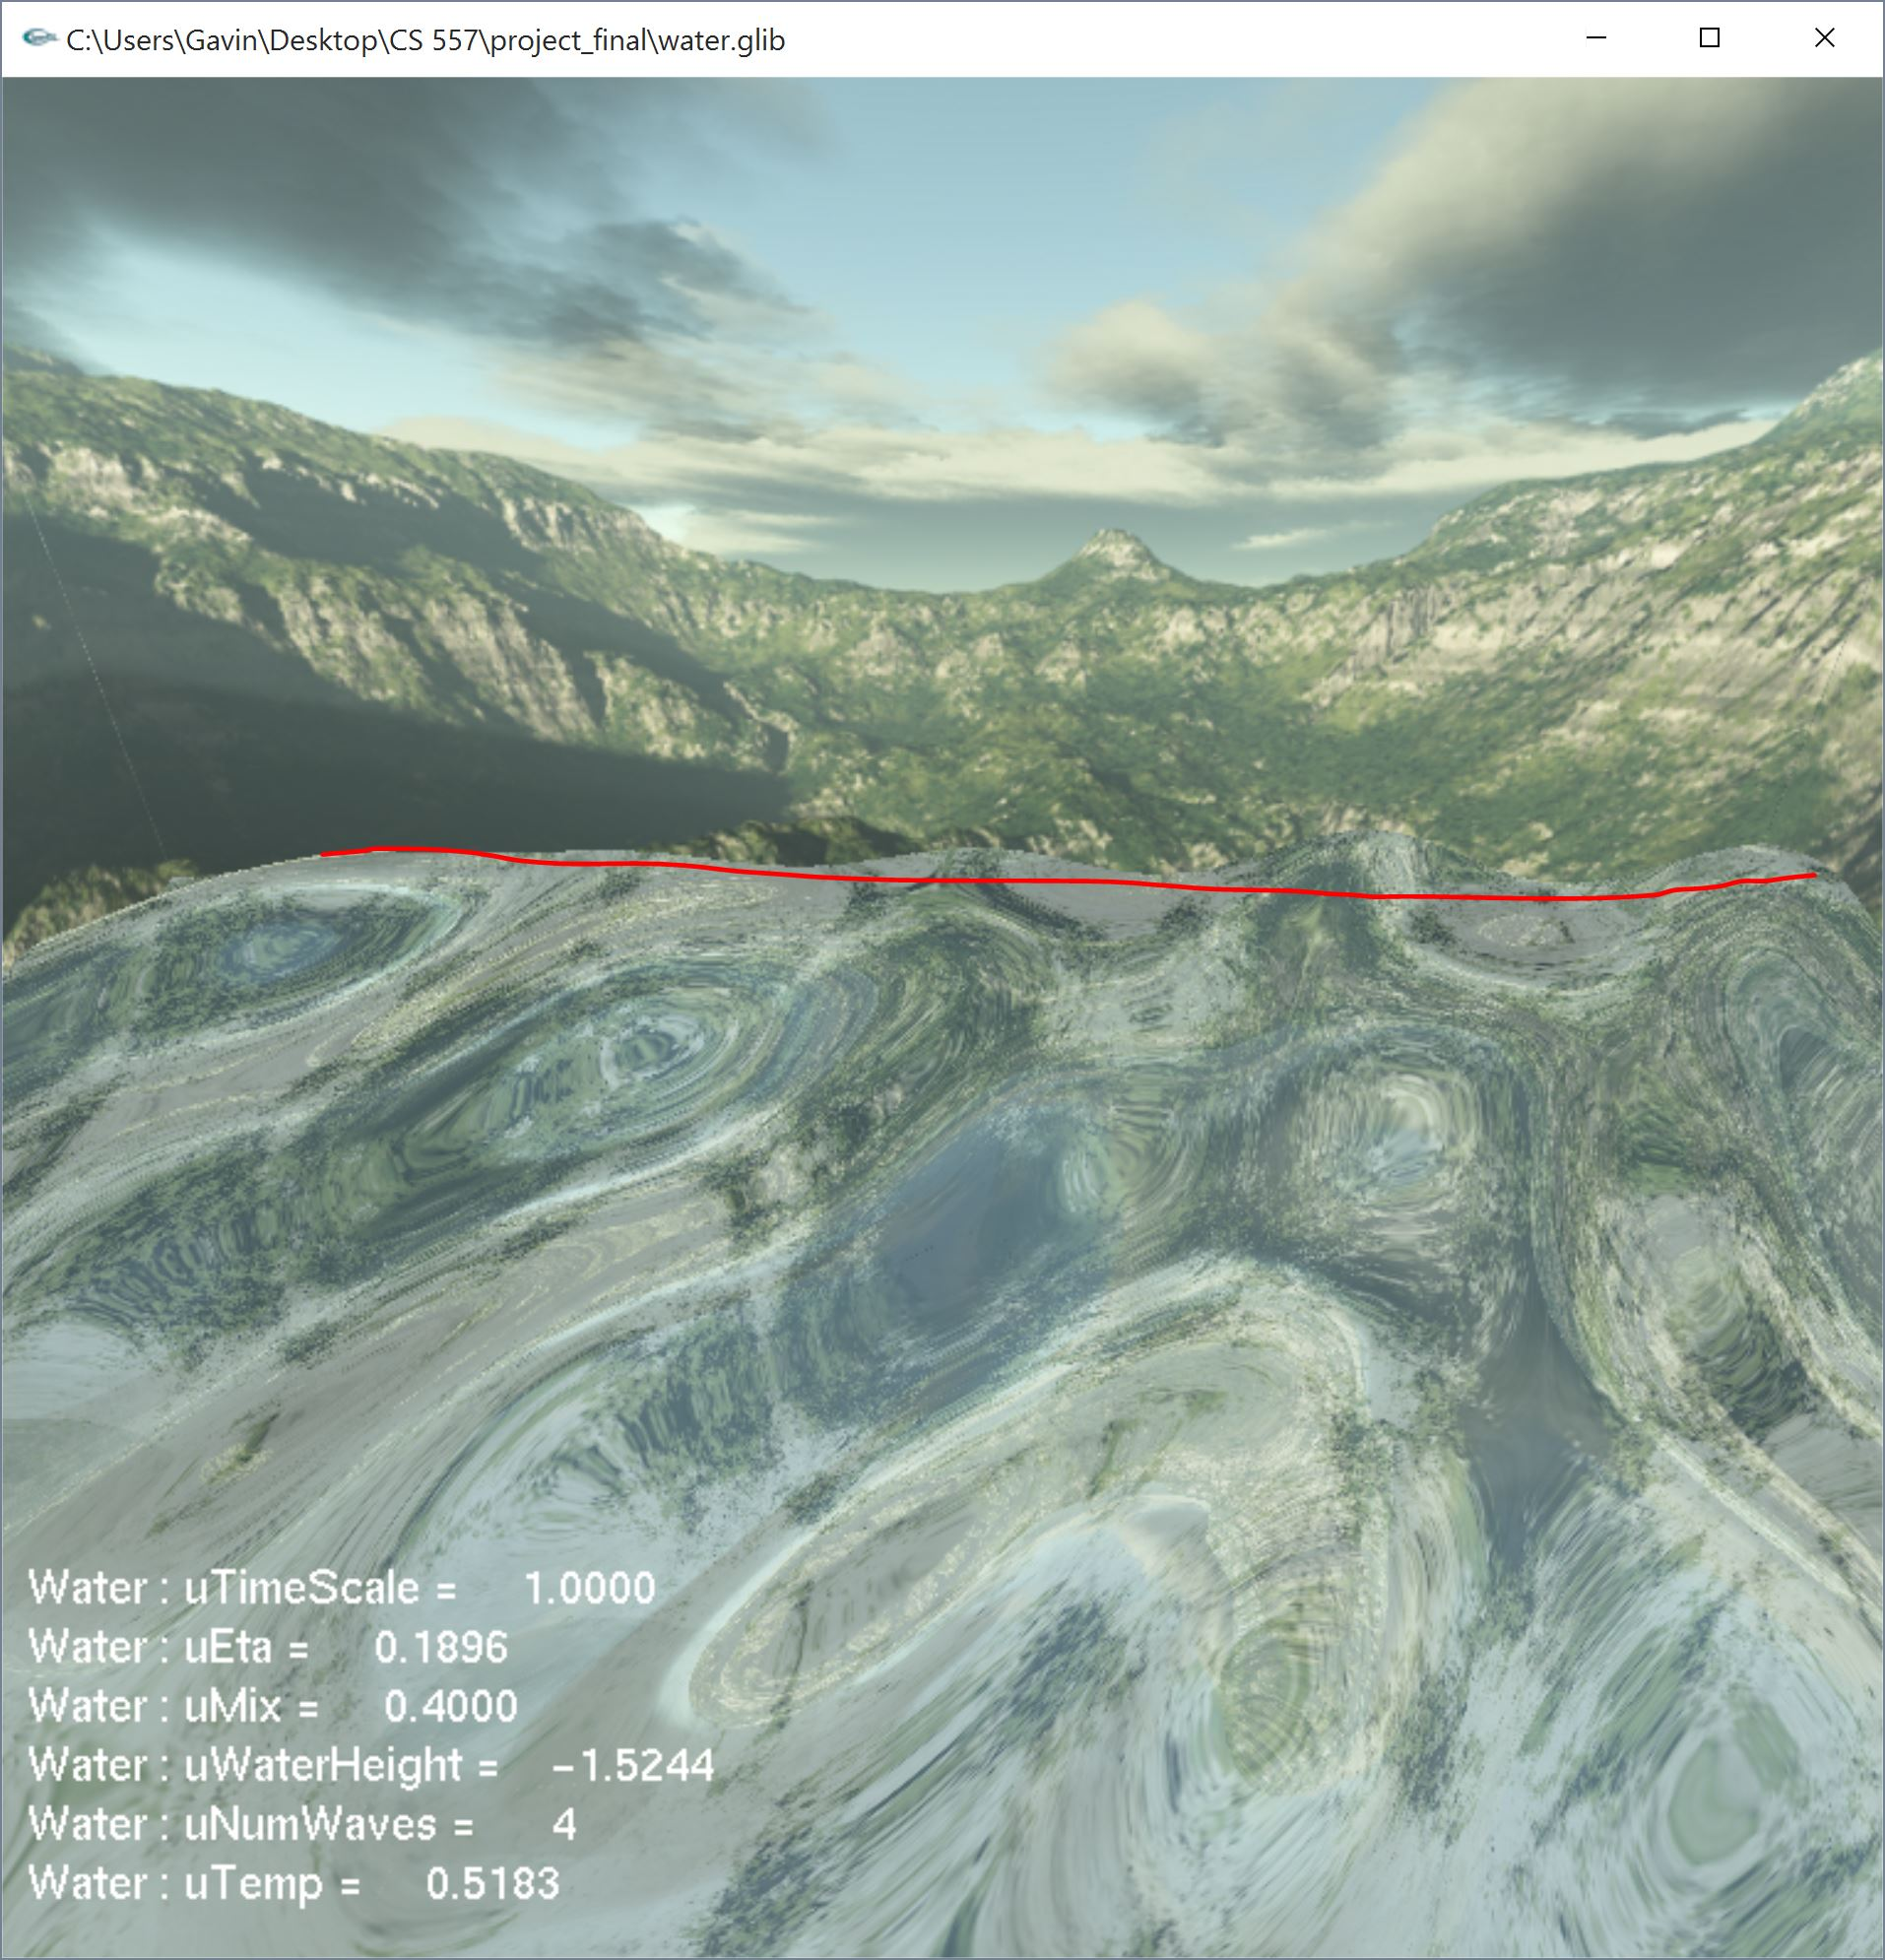
\includegraphics[width=2.8in]{heightwater.jpg}
	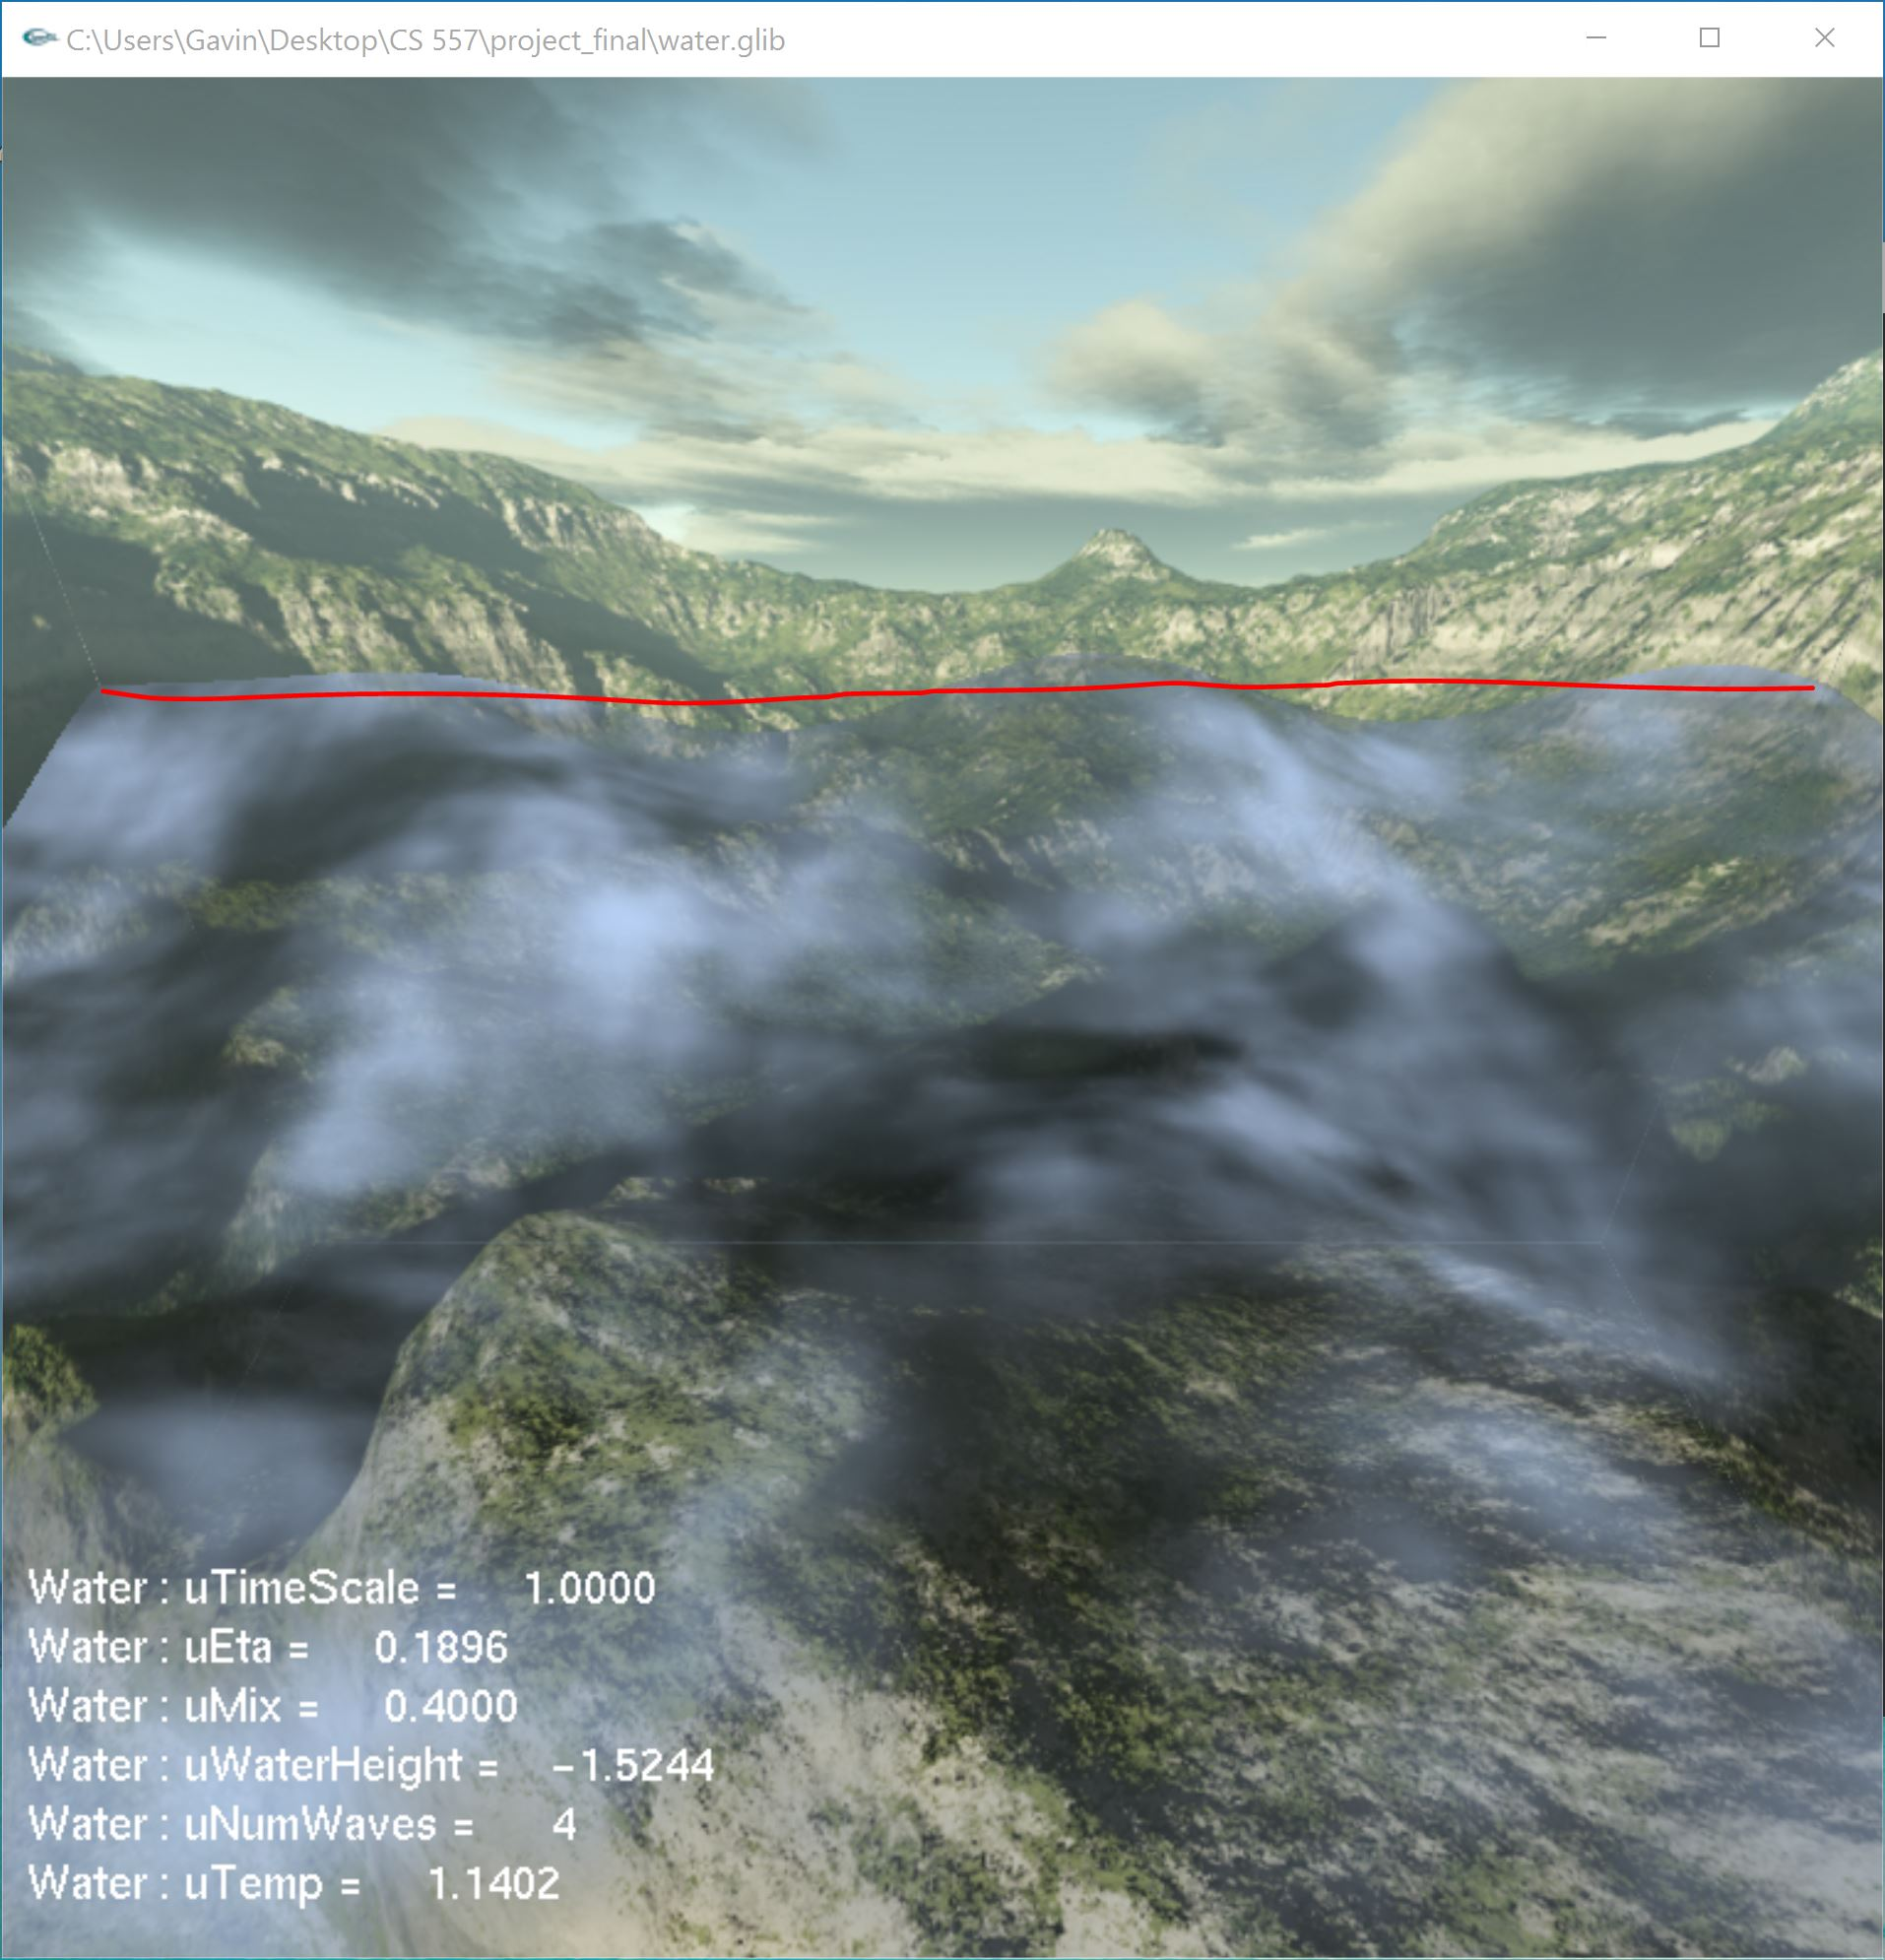
\includegraphics[width=2.8in]{heightcloud1.jpg}
	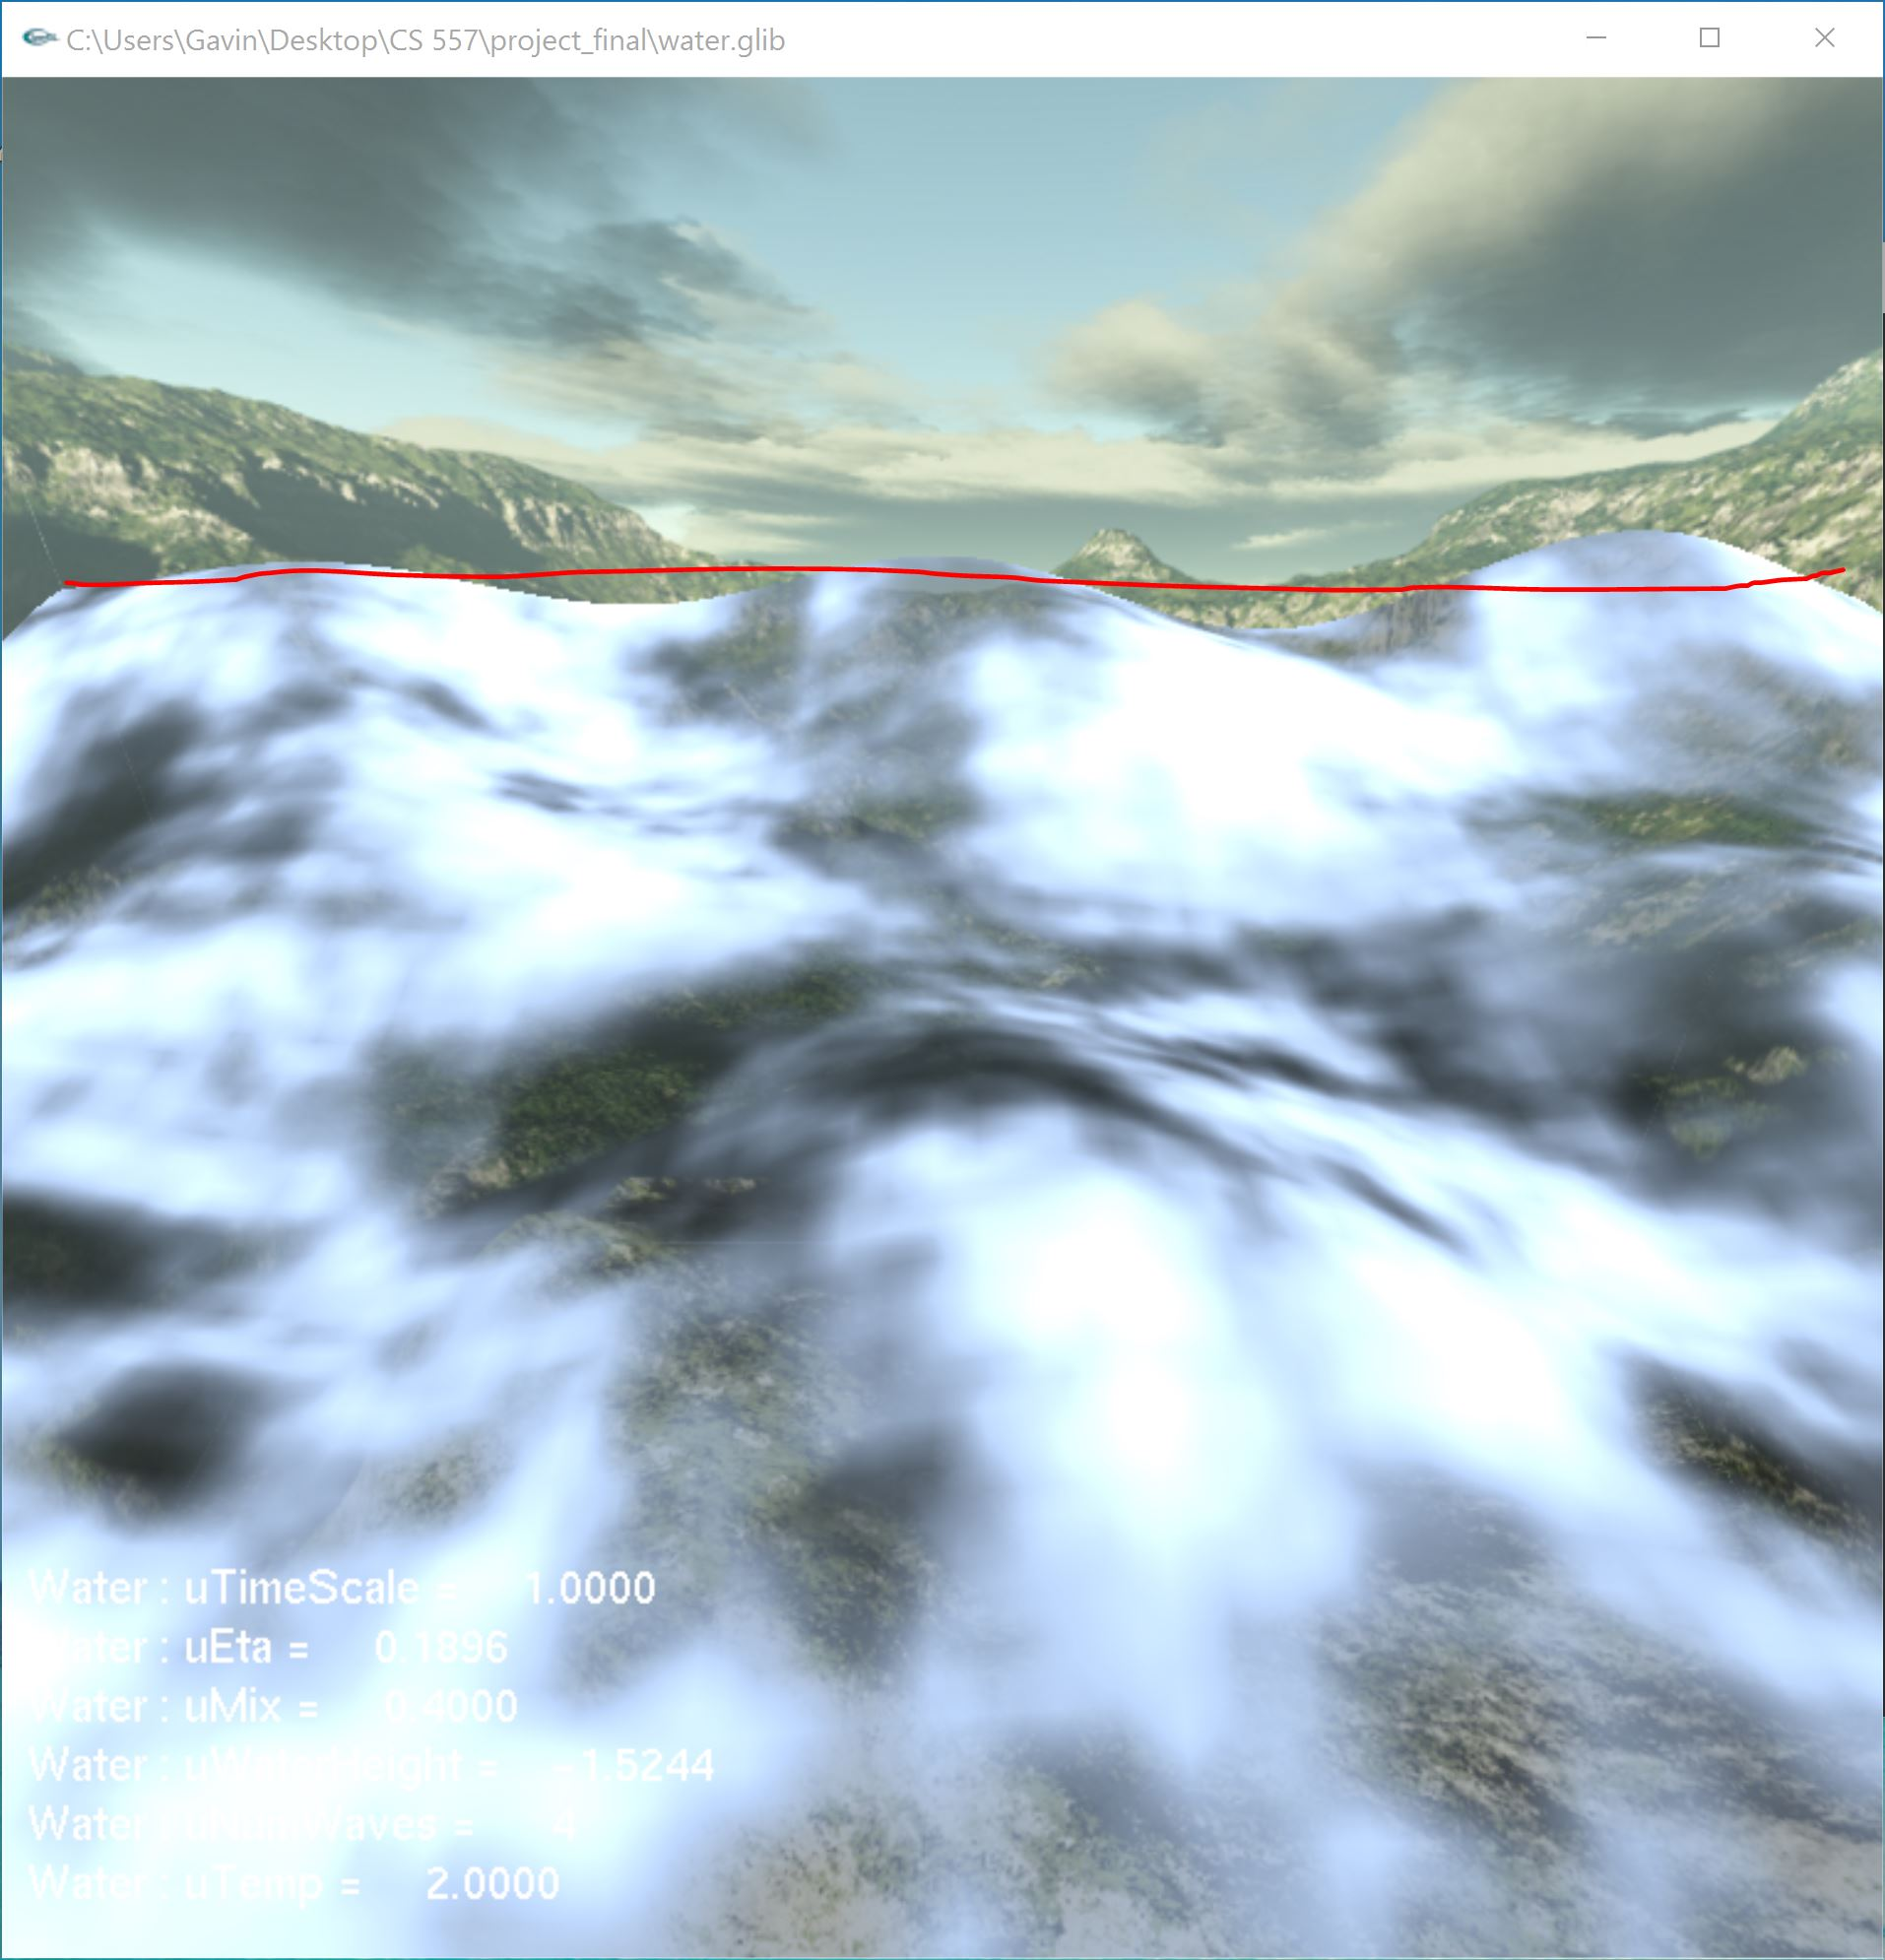
\includegraphics[width=2.8in]{heightcloud2.jpg}
\end{center}
Up till now, all of the features in the projects are introduced. The other features mentioned in the proposal such as the raining and the ripples are not implemented into this project due to the time issue. They could be treated as the future work of this project. However, the main part of the proposal, which is water morphological changes, is well implemented. This also has more space for development such as rendering the dynamic cloud instead of the pattern and they will also be treated as part of the future work. The following three images show the final result of the rendering. Hope you enjoy it!
 \begin{center}
 	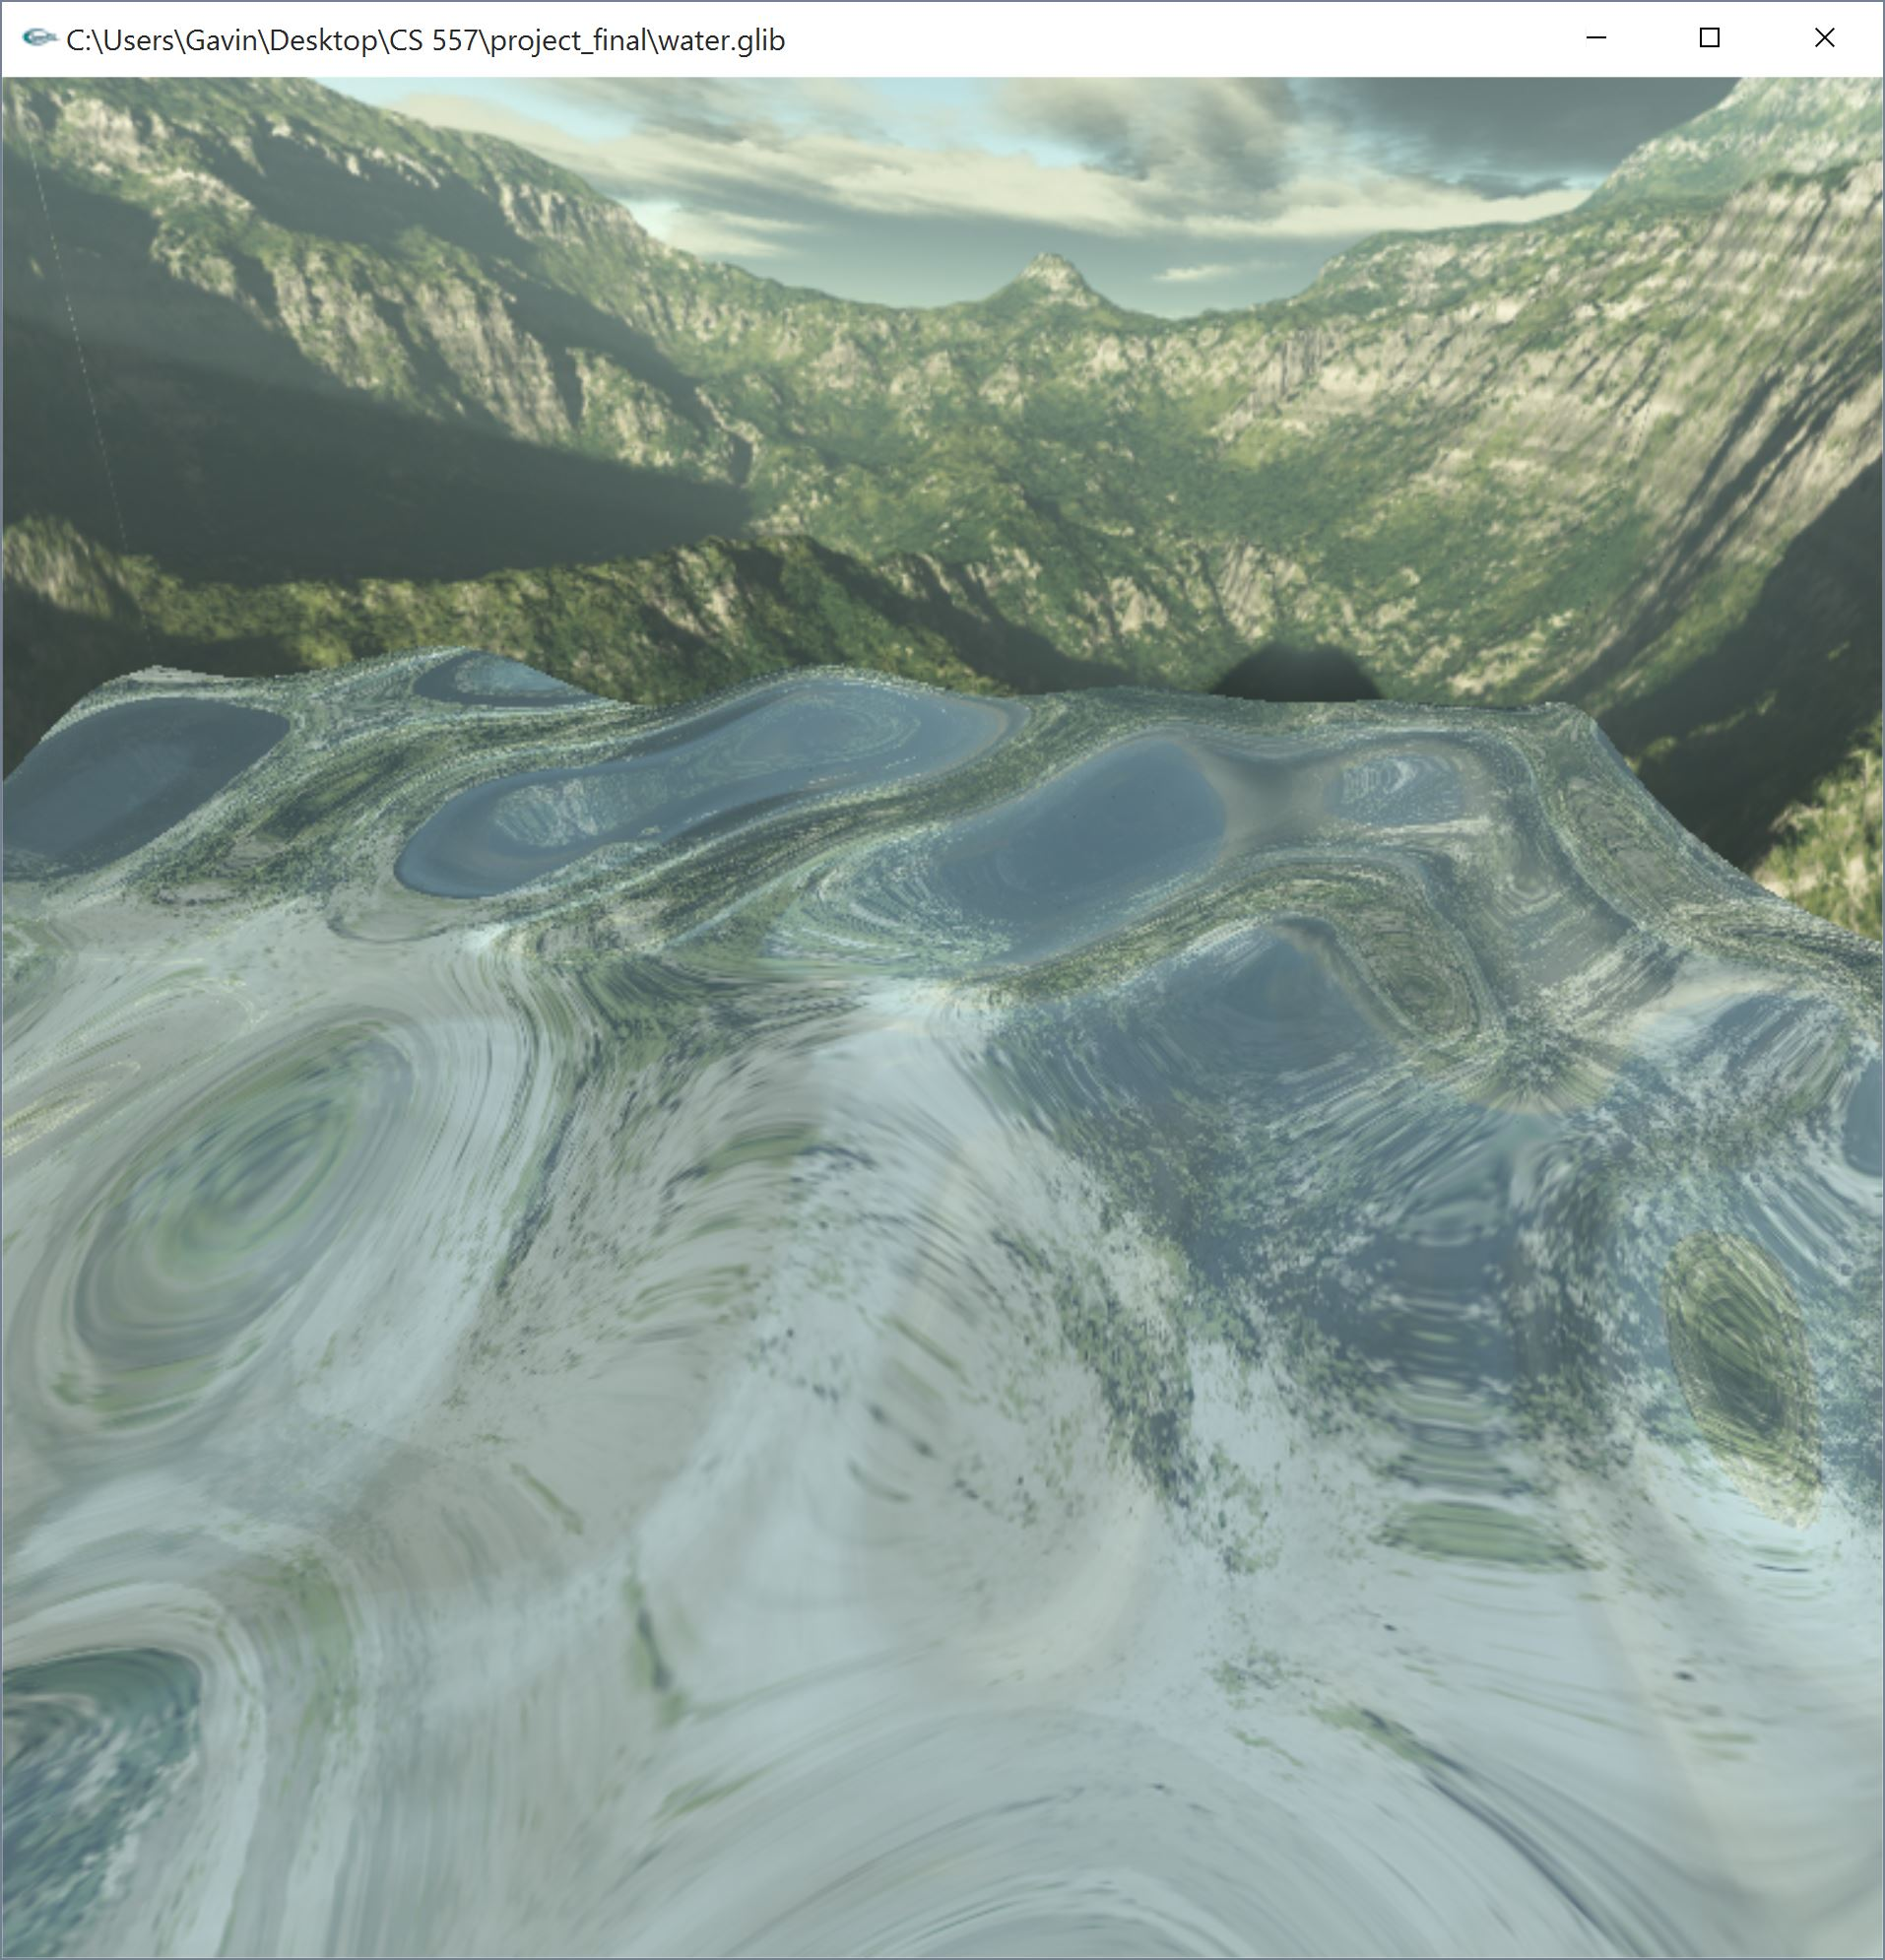
\includegraphics[width=4.25in]{final1.jpg}
 	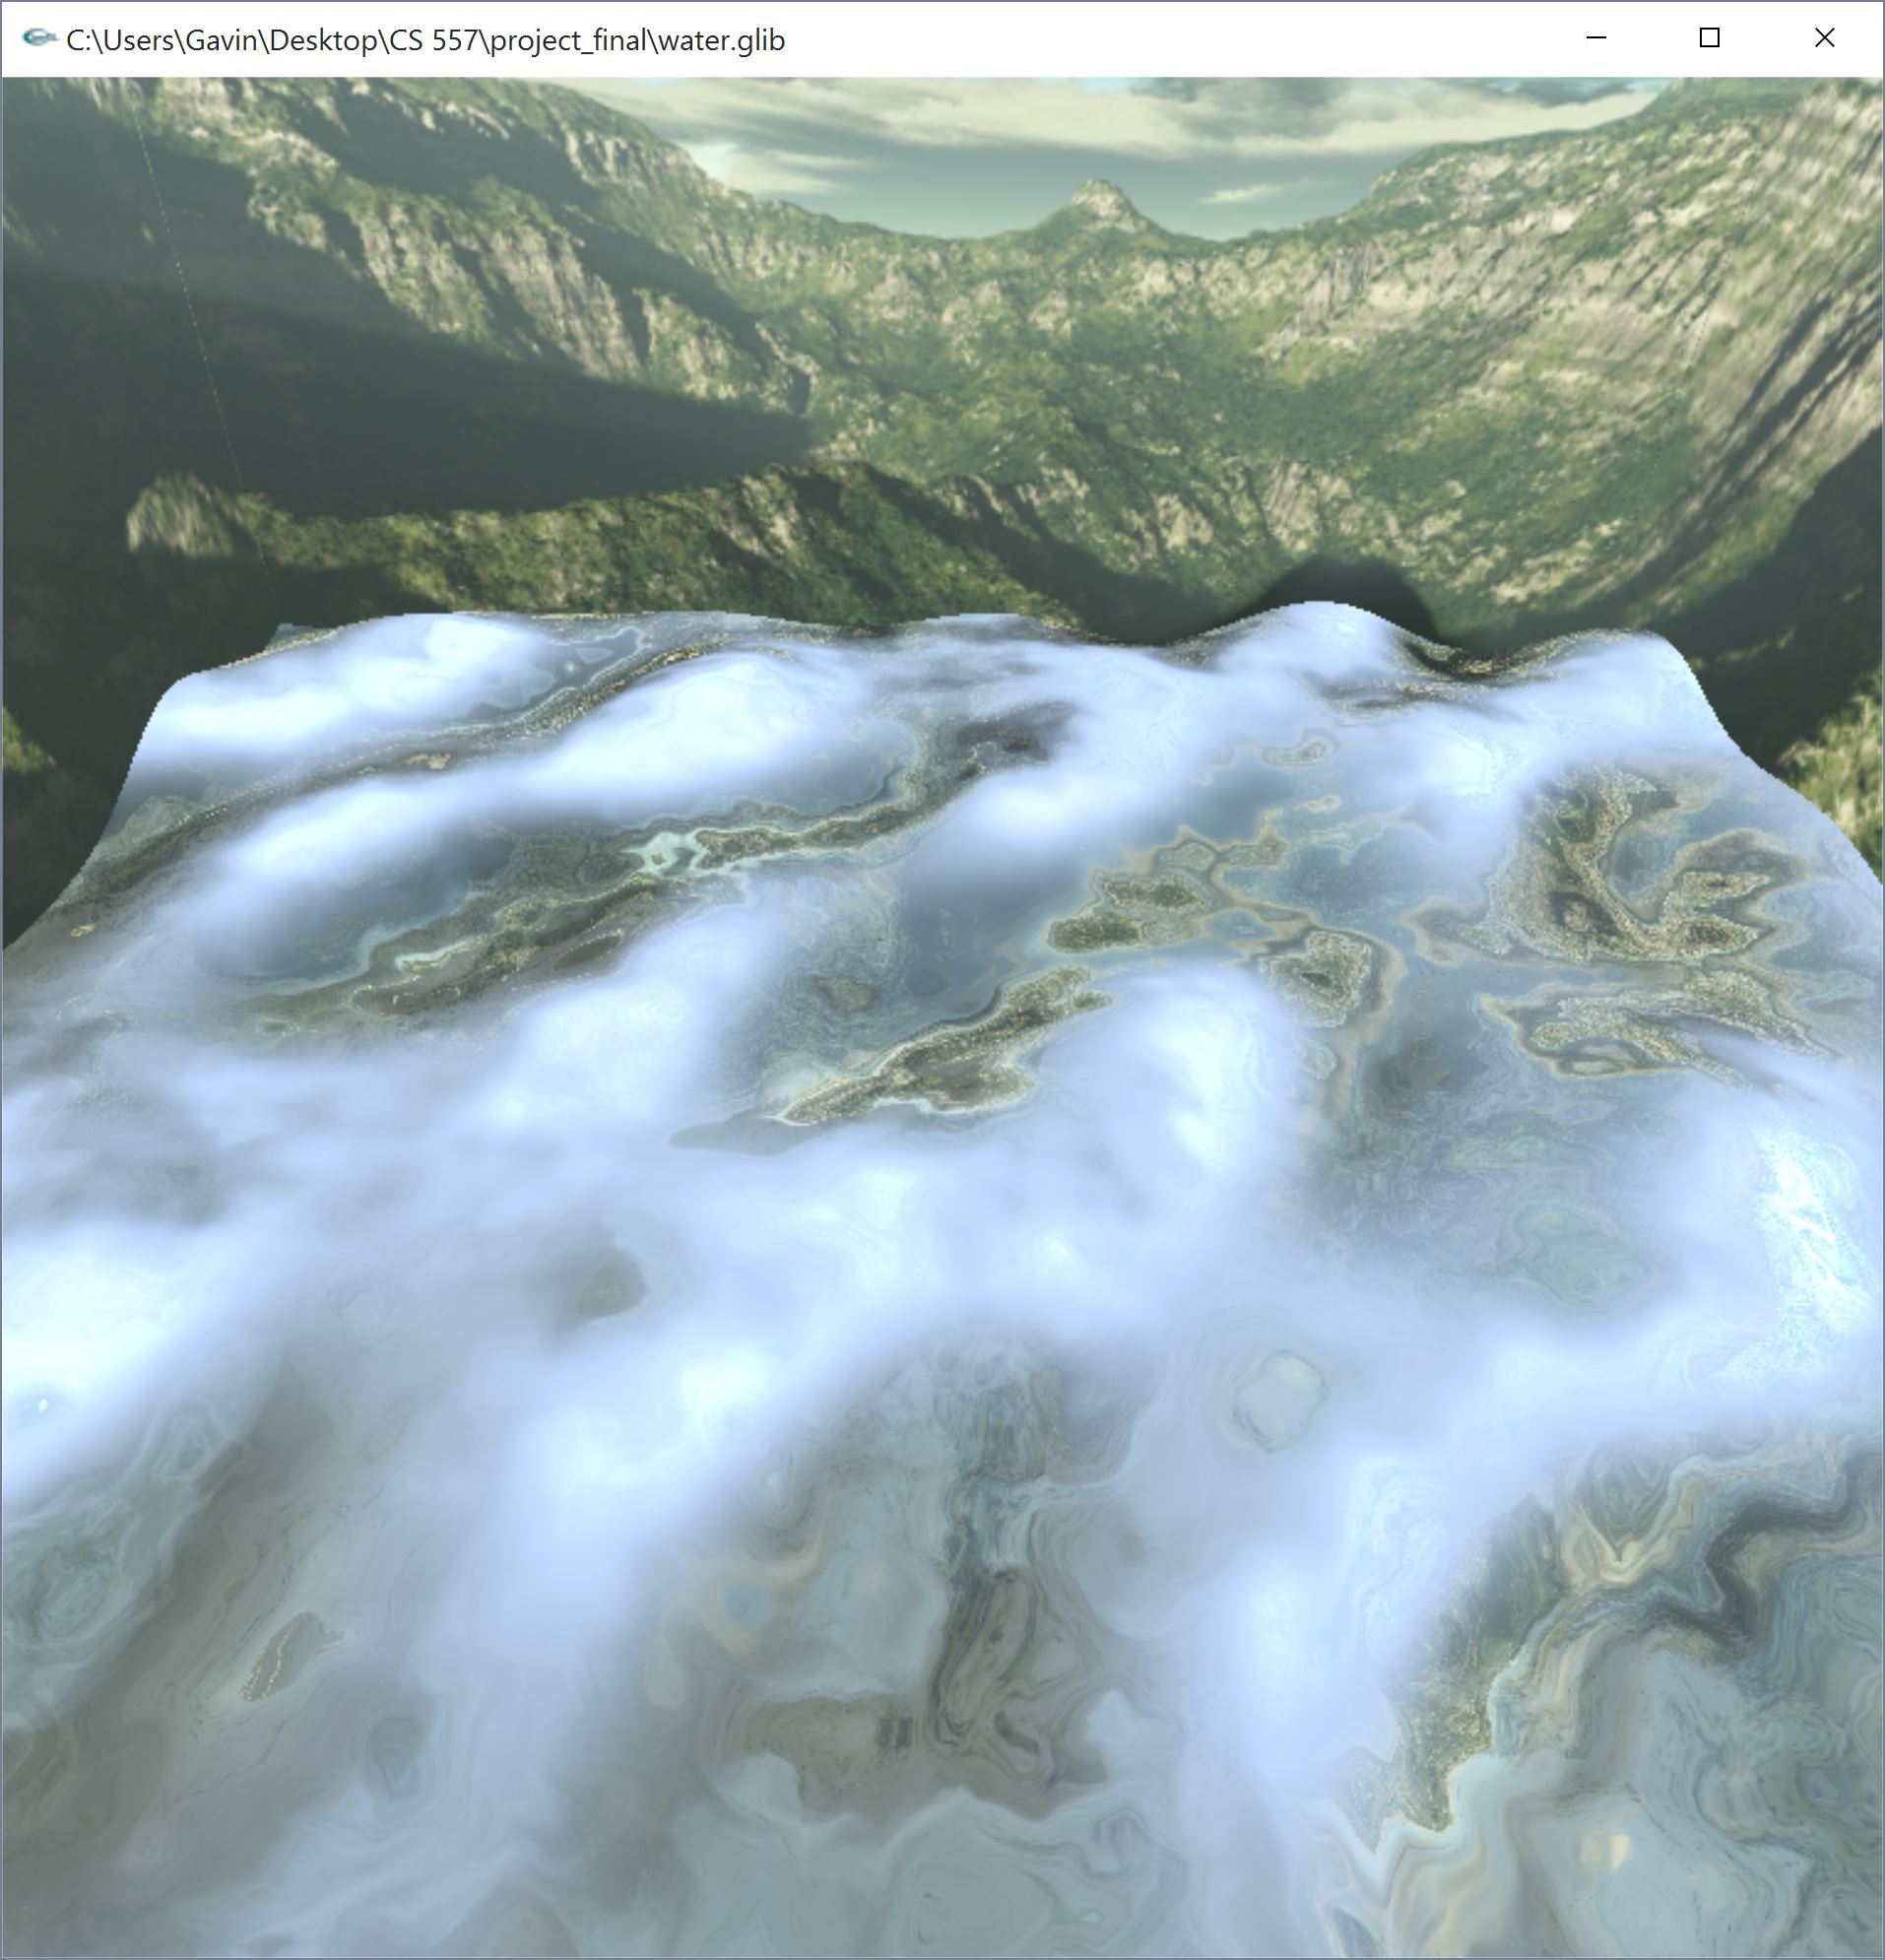
\includegraphics[width=4.25in]{final2.jpg}
 	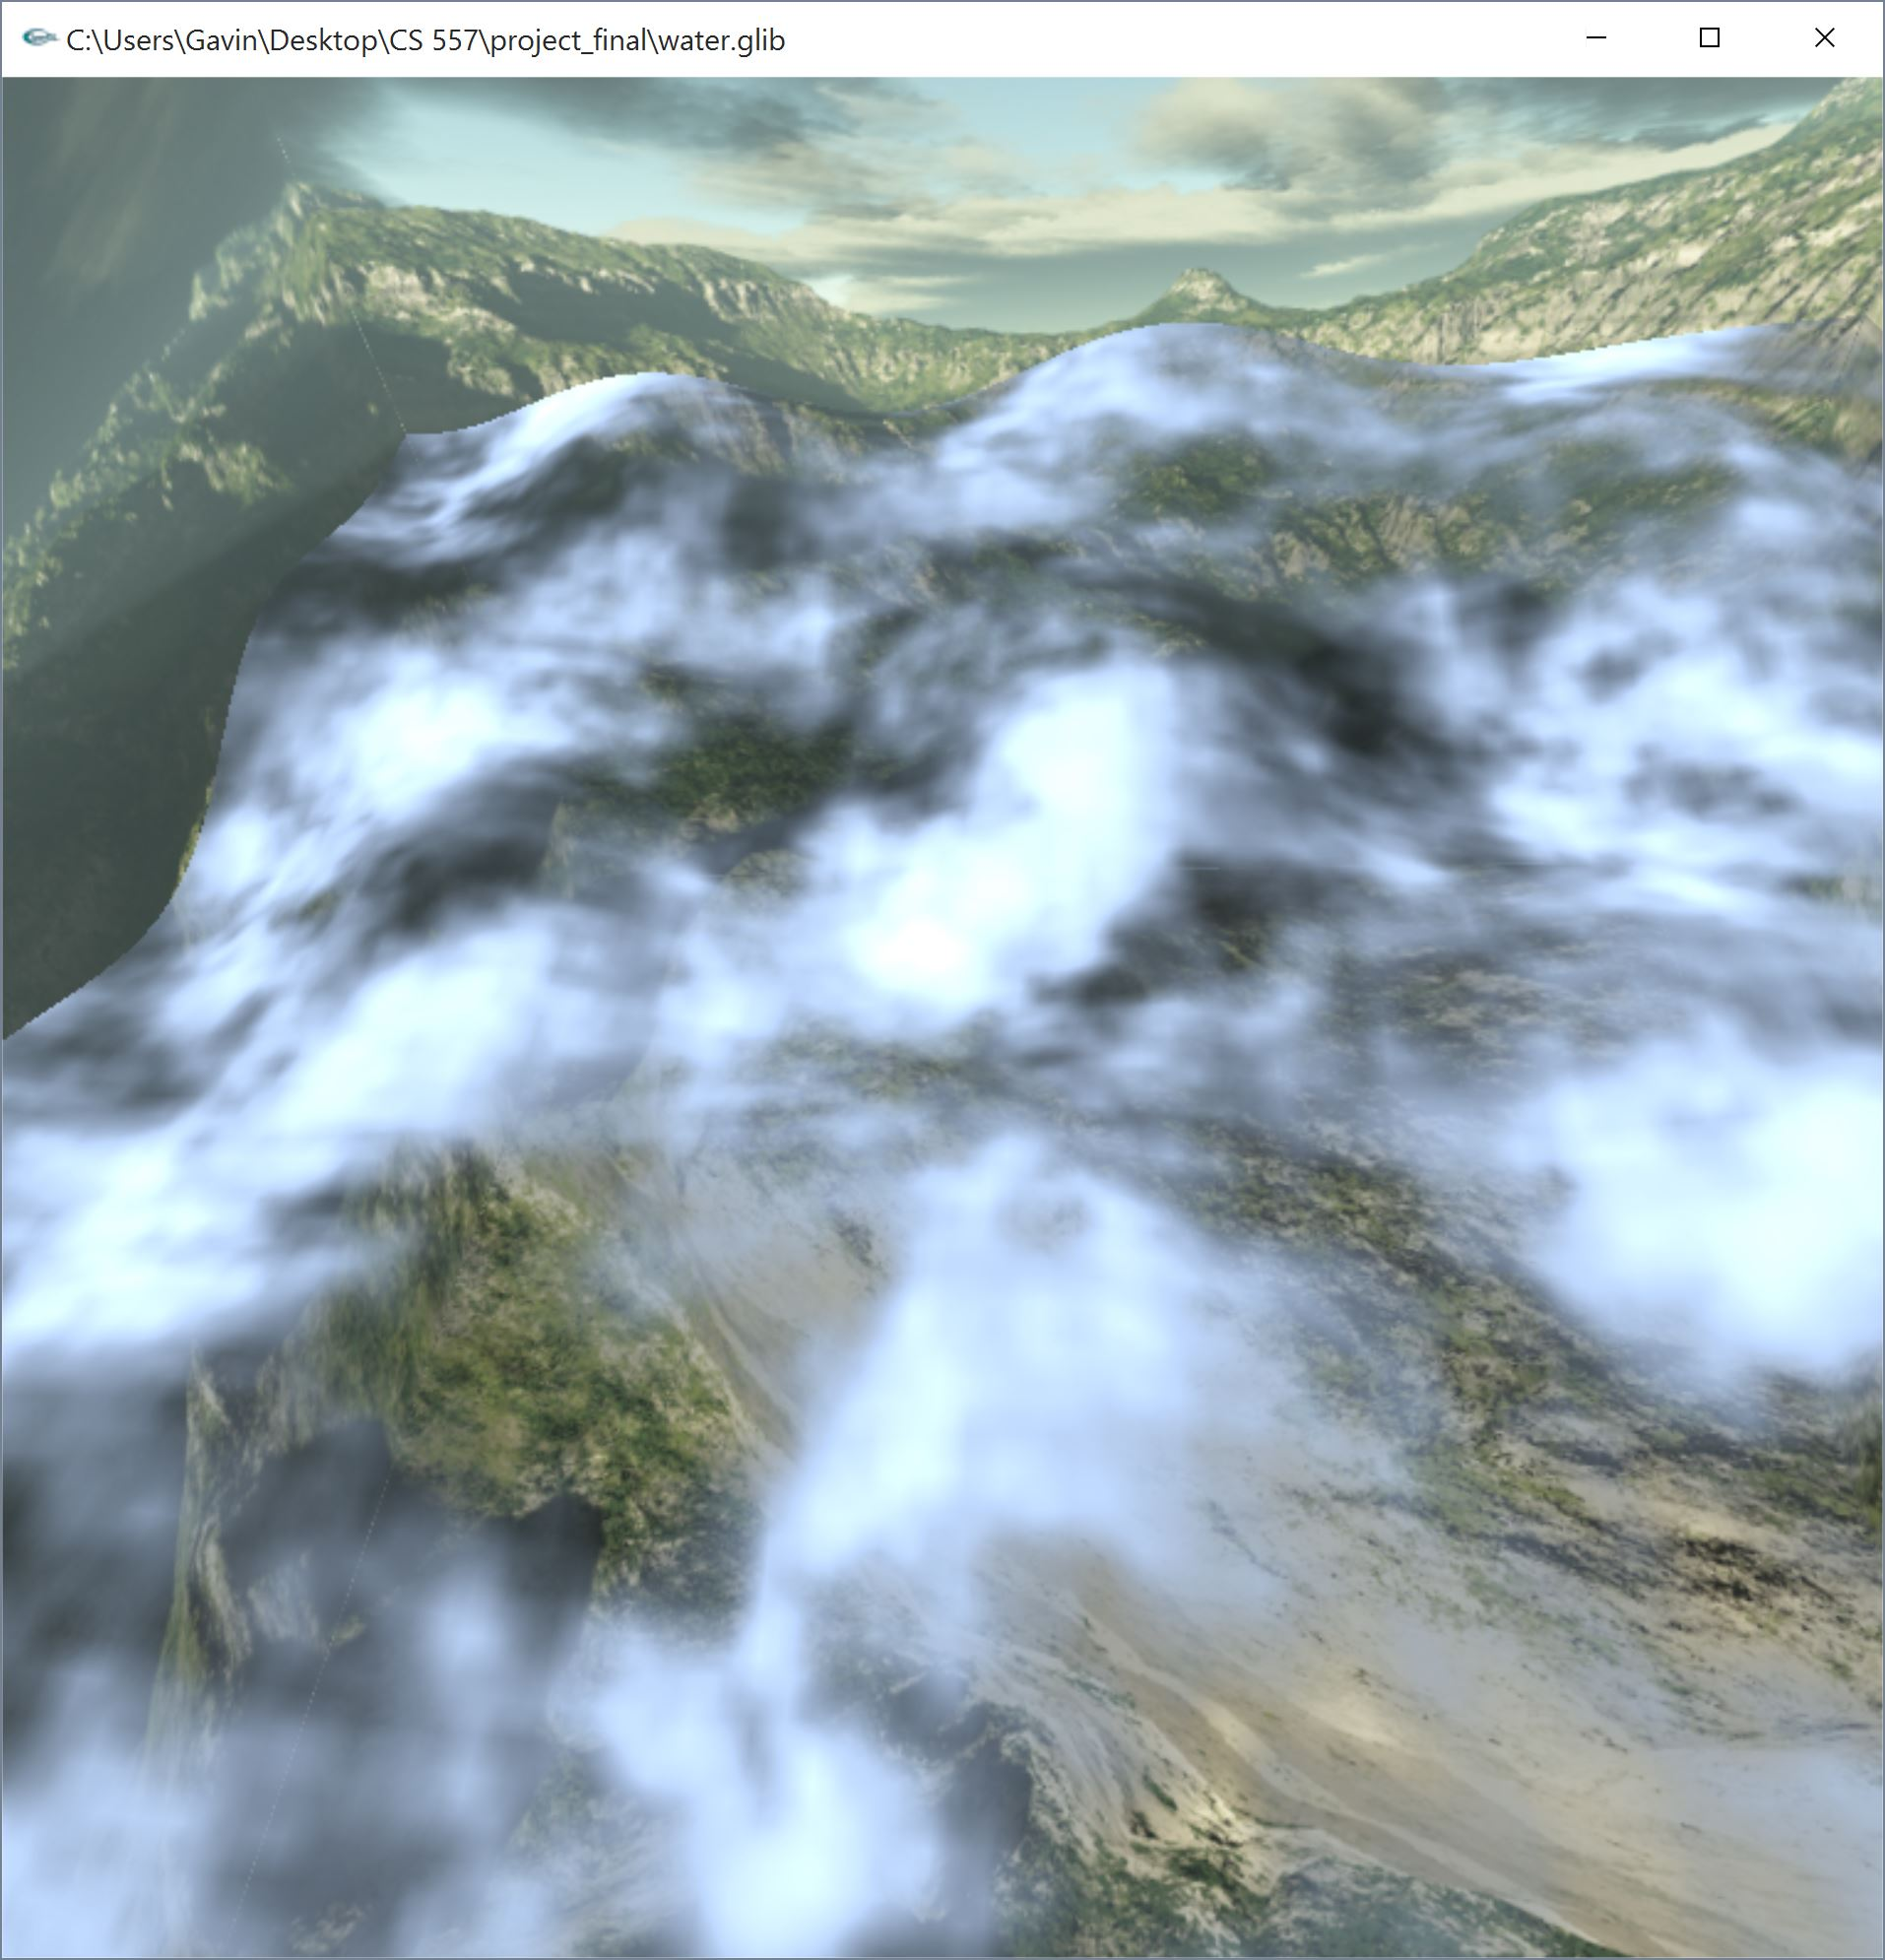
\includegraphics[width=4.25in]{final3.jpg}
 \end{center}
\section{Summary}
This is the last project of the shaders class, but it won't be the last shader project I write. To implement this project I did a lot research on how to do it, and I found that there exists a lot more things I need to learn out of the class, even though I have already learned so much during the class. By the end of the term I could present that I am familiar with shaders but I'm not going to statement that I am really good at it. After the class I will do more things with shaders and learn a lot more about them since I'm really interested in it. Hope I did well in this project and I will do a lot better than what I'm capable of right now. Hope you enjoy what I did in this project and the report.

\begin{thebibliography}{9}
	\bibitem{waterSimu}
	Jay Conrod,
	\emph{Water simulation in GLSL},
	jayconrod.com,
	\url{http://jayconrod.com/posts/34/water-simulation-in-glsl},
	2011-11-26.
	
	\bibitem{RealTime}
	Yunfei Bai,
	\emph{Real-time Water Rendering Using GPU},
	Georgia Institute of Technology,
	\url{http://www.cc.gatech.edu/~ybai30/cs_7490_final_website/cg_water.html}.
	
\end{thebibliography}
\end{document}